\documentclass[12pt, titlepage]{article}

\usepackage[margin = 1in]{geometry}
\usepackage{amsmath}
\allowdisplaybreaks
\usepackage{authblk}
\usepackage{setspace}
\usepackage{natbib}
\usepackage{hyperref}\hypersetup{colorlinks=true, citecolor=blue}
\usepackage{parskip}
\usepackage{textgreek}
\usepackage{graphicx}
\usepackage{booktabs} % For better looking tables
\usepackage{siunitx} % For alignment of numbers
\usepackage{placeins}
\usepackage{caption}  % For custom captions
\usepackage{float}   % Required for the H specifier
\usepackage{adjustbox}


\usepackage[]{lineno}
\linenumbers*[1]
%% patches to make lineno work better with amsmath
\newcommand*\patchAmsMathEnvironmentForLineno[1]{%
	\expandafter\let\csname old#1\expandafter\endcsname\csname
	#1\endcsname
	\expandafter\let\csname oldend#1\expandafter\endcsname\csname
	end#1\endcsname
	\renewenvironment{#1}%
	{\linenomath\csname old#1\endcsname}%
	{\csname oldend#1\endcsname\endlinenomath}}%
\newcommand*\patchBothAmsMathEnvironmentsForLineno[1]{%
	\patchAmsMathEnvironmentForLineno{#1}%
	\patchAmsMathEnvironmentForLineno{#1*}}%
\AtBeginDocument{%
	\patchBothAmsMathEnvironmentsForLineno{equation}%
	\patchBothAmsMathEnvironmentsForLineno{align}%
	\patchBothAmsMathEnvironmentsForLineno{flalign}%
	\patchBothAmsMathEnvironmentsForLineno{alignat}%
	\patchBothAmsMathEnvironmentsForLineno{gather}%
	\patchBothAmsMathEnvironmentsForLineno{multline}%
}

\sisetup{
  group-separator = {,},
  round-mode = places,
  round-precision = 0
}


% control floats
\renewcommand\floatpagefraction{.9}
\renewcommand\topfraction{.9}
\renewcommand\bottomfraction{.9}
\renewcommand\textfraction{.2}
\setcounter{totalnumber}{50}
\setcounter{topnumber}{50}
\setcounter{bottomnumber}{50}


\newcommand{\jy}[1]{\textcolor{orange}{JY: (#1)}}
\newcommand{\yh}[1]{\textcolor{purple}{YH: (#1)}}
\newcommand{\yx}[1]{\textcolor{cyan}{YX: (#1)}}
\let\proglang=\textsf
%% \newcommand{\pkg}[1]{{\fontseries{m}\selectfont #1}}
%% \newcommand\code[2][black]{\textcolor{#1}{\texttt{#2}}}

\title{Principles for Open Data Curation: A Case Study with the New
  York City 311 Service Request Data}


\author[1]{David Tussey}
\author[2]{Jun Yan}
\affil[1]{Former Executive Director, NYC DoITT}
\affil[2]{Department of Statistics, University of Connecticut}


\begin{document}
\maketitle

\tableofcontents % Optional: Table of Contents
\listoffigures % List of Figures
\listoftables % List of Tables

\hyphenpenalty=1000


\begin{abstract}
  Open data is important ...
  Quality control is important ...
  We use New York City 311 requests data  ...
  We suggest some open data quality control protocols ...


\bigskip
  
\noindent
{\it Keywords:}
consistency check;    
data release protocol;
data science;
open data;
data cleansing;
quality control	
\end{abstract}

\doublespacing

\section{Introduction} \label{sec:intro}

In the early 21st century, the open data movement began to take shape, driven by the 
fundamental belief that freely accessible data can transform 
both societies and governments. This movement champions the principles of 
transparency, innovation, and public engagement. 

A landmark in this journey was the launch of the United States'
\href{https://www.data.gov}{Data.gov} portal in 2009, a pioneering
platform in making government data widely accessible. Shortly after,
the European Union followed suit, unveiling its
\href{https://data.europa.eu/euodp}{Open Data Portal} in 2012, further
cementing the movement's global reach. Furthermore, the World Bank's Open
Data initiative, initiated in 2010, stands out as a comprehensive
repository for global development data, available at
\href{https://data.worldbank.org}{World Bank Open Data}. 

These initiatives represent significant strides in democratizing data, in breaking barriers that once
kept valuable information on government performance in silos. Their collective impact is profound, extending beyond
mere data sharing to fostering a culture of openness that benefits
individuals, communities, governments, and economies worldwide
\citep{barns2016mine, wang2016adoption}.

New York City (NYC) has emerged as a forerunner in the open data
movement, marked by the enactment of the Open Data Law in 2012
\citep{zuiderwijk2014open}. This landmark legislation led to the
creation of the \href{https://opendata.cityofnewyork.us}{NYC Open Data
  portal}, which today hosts an impressive array of 2700 datasets
from 80 different city agencies. This resource has become invaluable
for researchers in various fields as well an enabling local government transparency

In health, datasets have enabled
significant studies on facets of health and healthcare delivery
\citep{cantor2018facets, shankar2021data}. In the realm of urban
development, data has been instrumental in advancing smart city
initiatives \citep{neves2020impacts}. Additionally, transportation
research has benefited greatly from this wealth of data, aiding in the
understanding of urban mobility and infrastructure
\citep{gerte2019understanding}. NYC's Open Data initiative not only
exemplifies commitment to transparency and public engagement but also
illustrates how open data can be a powerful tool in addressing complex
urban challenges. Examples of some of the more popular NYC datasets include:

\begin{itemize}
	\item NYC restaurant violations
	\item Popular baby names
	\item Mapping of car crashes involving pedestrians
	\item Mapping of sidewalk widths in NYC 
	\item Visualization of NYC High School and College enrollment
	\item An interactive dashboard to filter and view charges for jail inmates
	\item Location of City-wide free Internet access points
	\item ...and 220 other complaint types. 
\end{itemize}

Data curation is fundamental in the open data ecosystem, ensuring the
utility and reliability of datasets for diverse applications. Among
the earliest discussions, \citet{witt2009constructing} focus on the
development of data curation profiles tailored to specific contexts,
setting a precedent for targeted data management
strategies. Addressing broader challenges in data sharing and
management, \citet{borgman2012conundrum} highlights the complexities
of research data distribution, emphasizing the need for robust
strategies. This is complemented by the work of \citet{hart2016ten},
who outline essential principles for effective data management,
particularly emphasizing the importance of meticulous curation
practices. 

In the realm of collaborative data management,
\citet{beheshti2019datasynapse} underscore the significance of
cooperative environments for managing and sharing social data
effectively. This aspect of data curation gains further relevance in
the research by \citet{mclure2014data}, which delves into the specific
practices and needs within data curation communities. The practical
implications of data curation are vividly illustrated in the context
of public health and global challenges. \citet{cantor2018facets}
demonstrate the utility of curated open data in evaluating community
health determinants. Furthermore, the COVID-19 pandemic serves as a
real-world example, with \citet{shankar2021data} observing the
critical role of collective data curation efforts in managing and
responding to the crisis. Collectively, these studies not only highlight the 
multifaceted nature of data curation but also emphasize
its indispensable role in enhancing the applicability and value of
open data across various domains.

The contributions of this paper are twofold. First, we delve into
the specifics of data curation challenges using the NYC 311 Service
Request Data as a case study. This renowned and frequently viewed 
dataset serves as a prime example for examining key issues in data curation, 
including data validity, consistency, and curation efficiency. 
We illustrate these points with live examples drawn from our processing of the 311 SR data. 

Secondly, building upon insights gained from this case study, we 
propose a set of data curation principles tailored for government-released open data. 
These principles are designed to address the unique challenges 
and requirements observed in the curation of such datasets.

The paper is organized as follows:
Section~\ref{sec:history} offers a brief review of the history of the 311 system. In 
Section~\ref{sec:trends} we take a look at long-term trends presented via a 10-year analysis.
Section~\ref{sec:issues} offers a general discussion of data cleansing issues
impacting data quality and curation efficiency. Section~\ref{sec:Structural} examines
the technical dimensions of the dataset, the structural issues. In Section~\ref{sec:datatypes} we examine the data fields
for compliance with the stated data type as found in the Data Dictionary. Section~\ref{sec:blanks} looks
at the data fields as regards missing, blank, or N/A entries. Section~\ref{sec:domain} explores
how data fields comply with a domain of legal or acceptable values. Section~\ref{sec:inconsistencies}
deals with the important issues surrounding logical inconsistencies and concerning patterns in the data. Section~\ref{sec:precision} 
explores the age-old issue of precision versus accuracy. Section~\ref{sec:duplicates}
identifies duplicate and redundant data fields. Section~\ref{sec:improvements} provides 
actionable suggestions for mitigating or resolving identified issues. Following this, Section~\ref{sec:protocol} outlines a series of general 
principles for the release of open data, drawing from our findings. The paper concludes with a discussion 
in Section~\ref{sec:discussion}, encapsulating the key insights and implications of our research.

A note on naming conventions: dataset field names are typically named using ``snake\_case'' where
each word in the variable name is written in lowercase, and words are separated by underscores,
e.g created\_date, complaint\_type, zip\_code, etc..   



\section{NYC 311 System History} \label{sec:history}

The NYC 311 service, a critical component of New York City's public
engagement and service response framework, serves as a centralized hub
for non-emergency inquiries and requests. Introduced in 2003, the NYC
311 system was designed to streamline the city's response to
non-emergency issues, ranging from noise complaints to street
maintenance requests. The evolution of this system can be traced from
its initial implementation as a simple inquiry channel via telephone to a
comprehensive data management system that handles millions of requests
annually. Each inquiry is logged as a complaint in the 311 system.
Key milestones in the 311 system development include:

\begin{itemize}
 	\item 2003 - NYC 311 system goes live with a phone-based call center only.
   	\item 2009 - 311 online \& mobile apps launched. Today 60\% of all Service Requests come from mobile \& online channels.
   	\item 2019 - Major software upgrade of 311 system with enhanced capabilities, dynamic load-balancing, and cloud-based resilience. 	
      \item 2020 - In August 2020, driven by the COVID pandemic, monthly 311 Service Requests hit an all-time high of 348,463. Seven of the Top 10 busiest days of all time occur in 2020.
      \item 2021 - 311 System is expanded to into the MTA's city subway system, the largest expansion since its inception.
   	\item 2023 - Record high year for 311 with 3.23 million Service Requests.
\end{itemize}

Today, the NYC 311 data system is a robust platform that manages a
vast array of urban living-related inquiries. The system handles over 3 million service 
requests (SRs) per year, encompassing such complaints as street noise, illegal parking, heat/hot water, abandoned vehicles,
and unsanitary conditions. The data, managed through a tailored application built on the Microsoft Dynamics and Azure platform, is a valuable resource for city
administration and policy-making. The 311 data is publicly accessible through the 
\href{https://opendata.cityofnewyork.us/}{NYC Open Data Portal} which provides access
to all the data sets (approx. 2700) and provides a convenient method for querying, grouping, aggregating, geo-mapping, visualization, and exporting
results. This open data initiative enables not only governmental transparency but also empowers 
researchers, civic developers, and the general public. 

Additional Open Data projects can be found at \href{https://opendata.cityofnewyork.us/projects/}{NYC Open Data Project Gallery}
and at \href{https://beta.nyc/beta/products/}{\textbeta etaNYC} products and tools.

Despite its success, the system constantly faces challenges such as:

\begin{itemize}
	\item Data timeliness, accuracy, and consistency
	\item Difficulties correlating data over long time periods, e.g. over a 10-year period, e.g. Agency name changes, new complaint types.
	\item Data anonymization and handling of Personally identifiable information (PII)
	\item Integration with stand-alone systems at selected NYC Agencies
	\item Managing API usage, authentication, and load for 3\textsuperscript{rd} party users, of which there are many
	\item Incorporating ongoing technology changes and upgrades 
	\item Understanding the role of chatbots and AI to provide online customer service, along with other emergent technologies
\end{itemize}

These and other challenges are continually addressed by the various Agency open data managers
as well as the \href{https://www.nyc.gov/content/oti/pages/}{NYC Office of Technology and Innovation (OTI)} which
provides the technology support for the open data system.  
Many of the underlying datasets are updated daily, usually running 1-2 days behind from creation.
However, a number of datasets are updated monthly (such as restaurant inspections), and some are
not updated for one or more years (such as community board boundaries). This poses problems when 
merging dataset with others, as would be expected. Typically, the data must be
exported and manipulated in another, external program. The authors found this to be the case with 
the large 311 dataset employed.

Data accuracy and consistency is typically established between OTI and the other contributing
City Agencies, such as NYPD, Housing Preservation and Development (HPD), Parks \& Recreation, etc.,
via Service Level Agreements (SLAs). However, enforcement of those SLAs is often challenging. The 
result is that often data accuracy and logical consistency is occasionally compromised. However, the Open Data
Team is quite responsive to inquires from users. The authors have provided many such 
suggestions during the course of this research effort, and the most current data shows improvements
in many of the areas highlighted. Questions and suggestion  can be provide here: 
\href{https://opendata.cityofnewyork.us/engage/}{Contact Us}.

The NYC 311 organization, part of OTI, operates a highly tailored and sophisticated case
management. However, one constraint was particularly challenging during the recent complete overhaul
of the software and hardware in 2019. When the original 311system was developed in 2003, 
a decision was made to allow select NYC Agencies to maintain their own local computer systems, 
such as the mainframe systems at the NYC Department of Sanitation (DSNY) and others. 
And when the 311 system was completely upgraded in 2019, those
same integrations were honored in order to reduce the scope of the project. Perhaps in
retrospect, while a good budgetary and policy decision, it was perhaps not such a good technology decision.

At least nine NYC Agencies have local systems that are integrated directly to the 311 system either via
an API or custom code. These include:

\begin{itemize}
	\item Department of Social Services (DSS), one of the largest City Agencies
	\item Department of Sanitation, although recently part of DSNY has moved to the core 311 software.
	\item Department of Parks \& Recreation (forestry complaints only)
	\item Housing, Preservation \& Development (fully integrated)
	\item Department of Environmental Protection (DEP) (fully integrated)
	\item Department of Healthy \& Mental Hygiene (fully integrated) 
	\item Department of Consumer \& Worker Protection (DCWP - formerly known as the Dept of Consumer Affairs)
	\item New York Police Department (NYPD) (integrated with their reporting system)
	\item Department of Business (DoB) (fully integrated)
\end{itemize}

One unfortunate side-effect from these integrations, and other Agencies that use the 311 APIs, is that some of the data consistency
checks which are inherent in the 311 system are not applied uniformly, and in some cases not at all, to the integrated data streams.
Errors often creep in from other Agency systems and are not easily corrected or detected in the 311 application itself,
but rather require correction at the source Agency; challenging.

One area that will almost certainly remain an ongoing issue is the ongoing incorporation of new software, hardware,
and cloud services which are constantly changing while new approaches emerge. The 311 telephonic integration recently was reconfigured due to a new
telephonic vendor. Desktop software at the 311 Agency are subject to the same upgrades that home and business users experience. And while the 
311 system was designed to be easily configured and updated with new features, some emerging business issues as well as
technologies nonetheless require additional software engineering efforts to accommodate, along with the concomitant budgets.

One area in particular which is heavily influencing customer outreach for the 311 system is the appropriate use of
online chatbots and assistants. Increasing these features are influenced by artificial intelligence (AI) advances. It is a given that
a number of citizen's interactions with City government could be handled accurately and quickly by AI-driven
applications thus improving timeliness and accuracy. But how to do that while preserving customer privacy and anonymization
and user engagement are challenging issues. 	

The impact of the NYC 311 data extends beyond operational efficiency;
it has become instrumental in shaping City governance and community
engagement. The data has been pivotal in such areas as:

\begin{itemize}
	\item Providing advice on shelters during hurricanes, heat emergencies, and winter blizzards
	\item Handling countless inquires during the COVID pandemic (testing centers, vaccine sites, mobile vaccine clinics, etc.)
	\item Enforcement of standards between landlords and tenants
	\item Re-allocation of NYC's yellow taxi routes based upon an insightful analysis conducted by the Taxi \& Limousine Commission (TLC)
	\item Improved responsiveness for City Agencies with regards to direct client-facing responsibilities such as Parks \& Rec, Dept of Transportation, DSNY, etc.
	\item Increased 311 SRs related to Homelessness resulted in the launch of the City's Homeless Outreach \& Mobile Engagement Street Action Teams (HOME-STAT)
	which includes street canvassers and increases in homeless housing facilities.
	\item A significant increase in graffiti complains in 2017 led directly to the `Graffiti-Free NYC'' campaigns and increased funding for removal of graffiti in public spaces.
	\item Enhanced geospatial data regarding the location of incidents, the responding Agency, and actions taken across a myriad of complaint\_types
	\item Establishment of Agency SLAs in regard to certain complaint types, such as residential noise, homelessness person assistance, street light outages, 
	rat sightings, and other neighborhood quality of life issues.
\end{itemize}

The NYC 311 service exemplifies the dynamic nature of urban data
management and its critical role in modern governance. In addition it provides an
invaluable resource for data scientists to practice data science activities, including data curation.

We extracted 311 SR data for the period of CY 2022-2023, a dataset consisting of
6.4 million records. That dataset serves as the primary source for the analysis effort. This is a large dataset which enables 
observation of some rarely seen events, data inaccuracies, and logical inconsistencies. It provides enough data to examine trends and data outlier analysis. 
We queried the data directly from the NYC Open Data Portal and then exported the data in CSV format for analysis using custom written R programs.

Additionally, we extracted two longer-term datasets, a 5-year look (2019-2023) and a 10-year look (2014-2023) ; some 14 and 27 million rows respectively. 
These larger datasets afford an opportunity for long-term trend observations, confirming and supporting the analysis using the 2-year dataset. The 2022-2023 dataset
was used exclusively for the detailed, field-by-field level analysis which comprises the majority of this effort. 



\section{10-year Analysis \& Trends} \label{sec:trends}

Since the NYC 311 System went live in 2003, the usage has grown at an annual
rate of 4.6\%. For this study, we also looked at a 10-year period (2014-2023) to
observe certain system performance characteristics over a longer time-frame . 
During that time-frame, the number of 311 SRs grew 50\% as shown in the chart below showing yearly SR counts.

\begin{figure}[H]
  \centering
  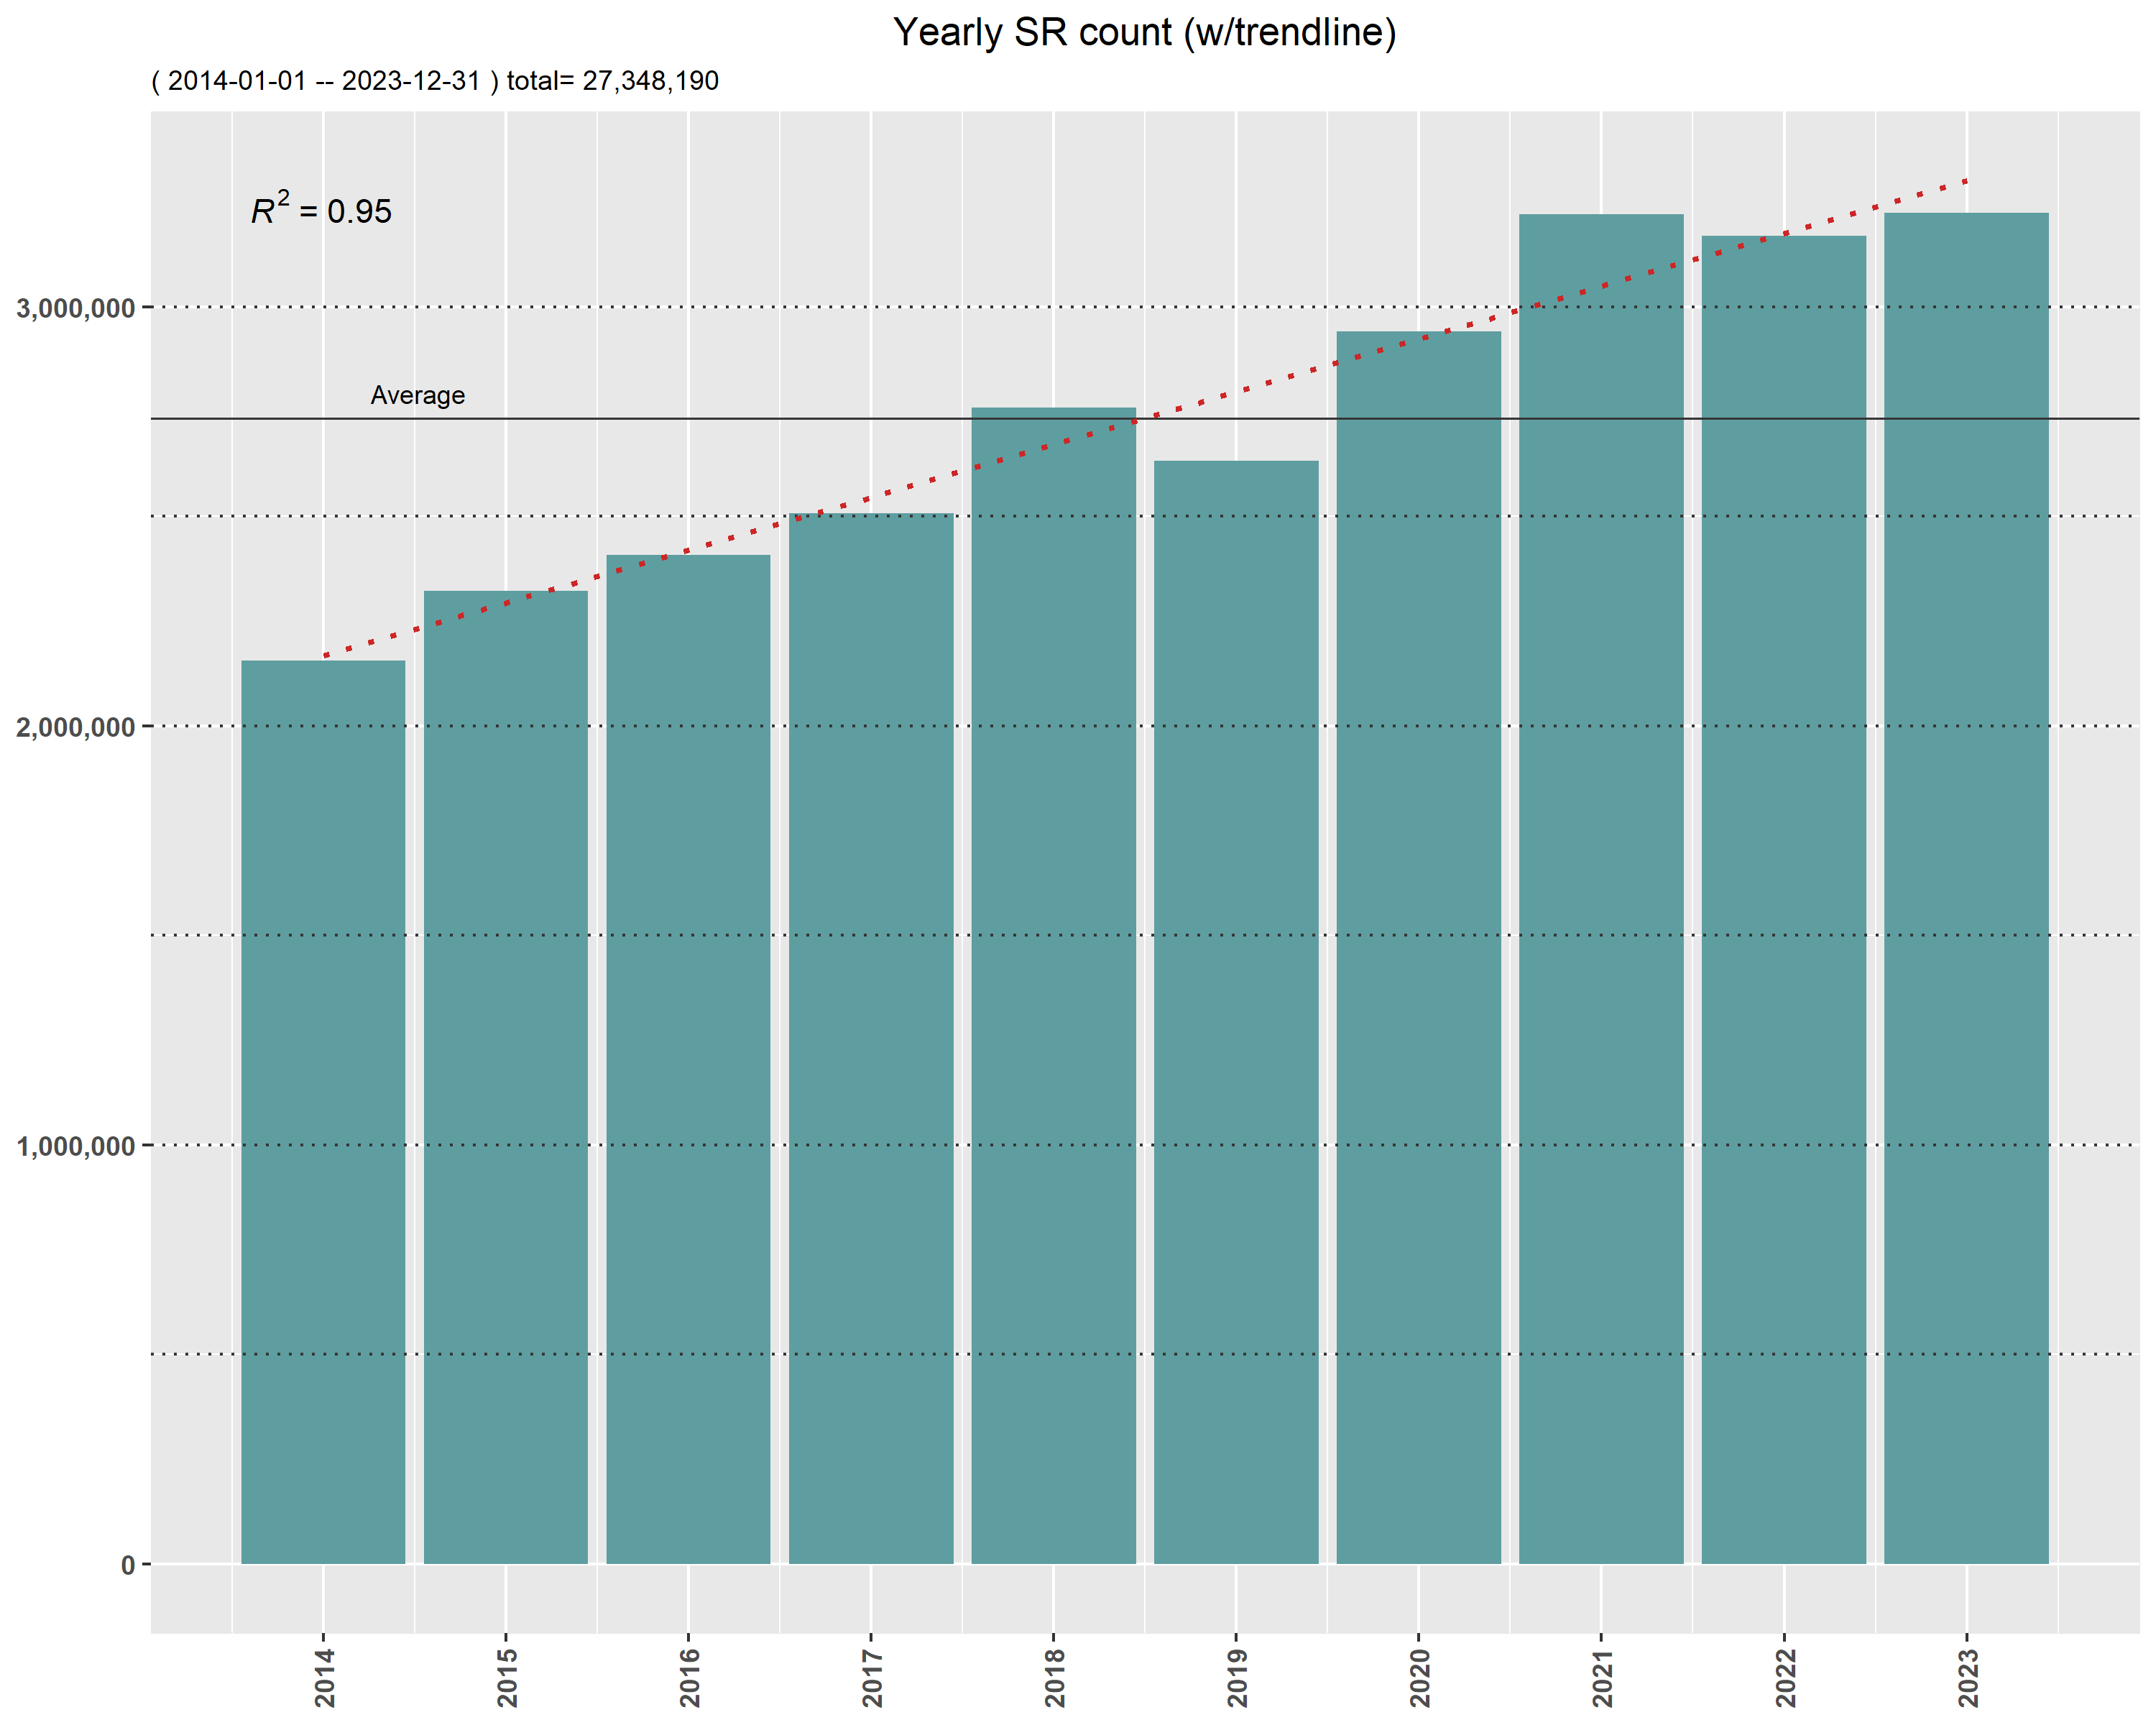
\includegraphics[width=\textwidth]{Yearly.png}
  \caption{Yearly SR counts over 10-year period}
  \label{fig:yearly-counts}
\end{figure}

This 10-year timeframe (2014-2023) included the COVID pandemic impact. Note that the pandemic
impact reached a peak in the July-September 2020 timeframe, accompanied by additional spikes
in the 2\textsuperscript{nd}half of 2021 as well. The all-time daily high for SRs occurred on Tuesday, 2020-08-04, with a spike of
24,415 SRs, a full 9.8 \textsigma's from the mean. 

This below chart shows the 10-year period by calendar month. Note that almost all the months before the COVID pandemic outbreak in Feb/Mar
of 2020 are ``below average'', while most of the months after that period are ``above average'' months. And that trend of higher usage
of the 311 system has continued into the early months of 2024.

\begin{figure}[htbp]
  \centering
  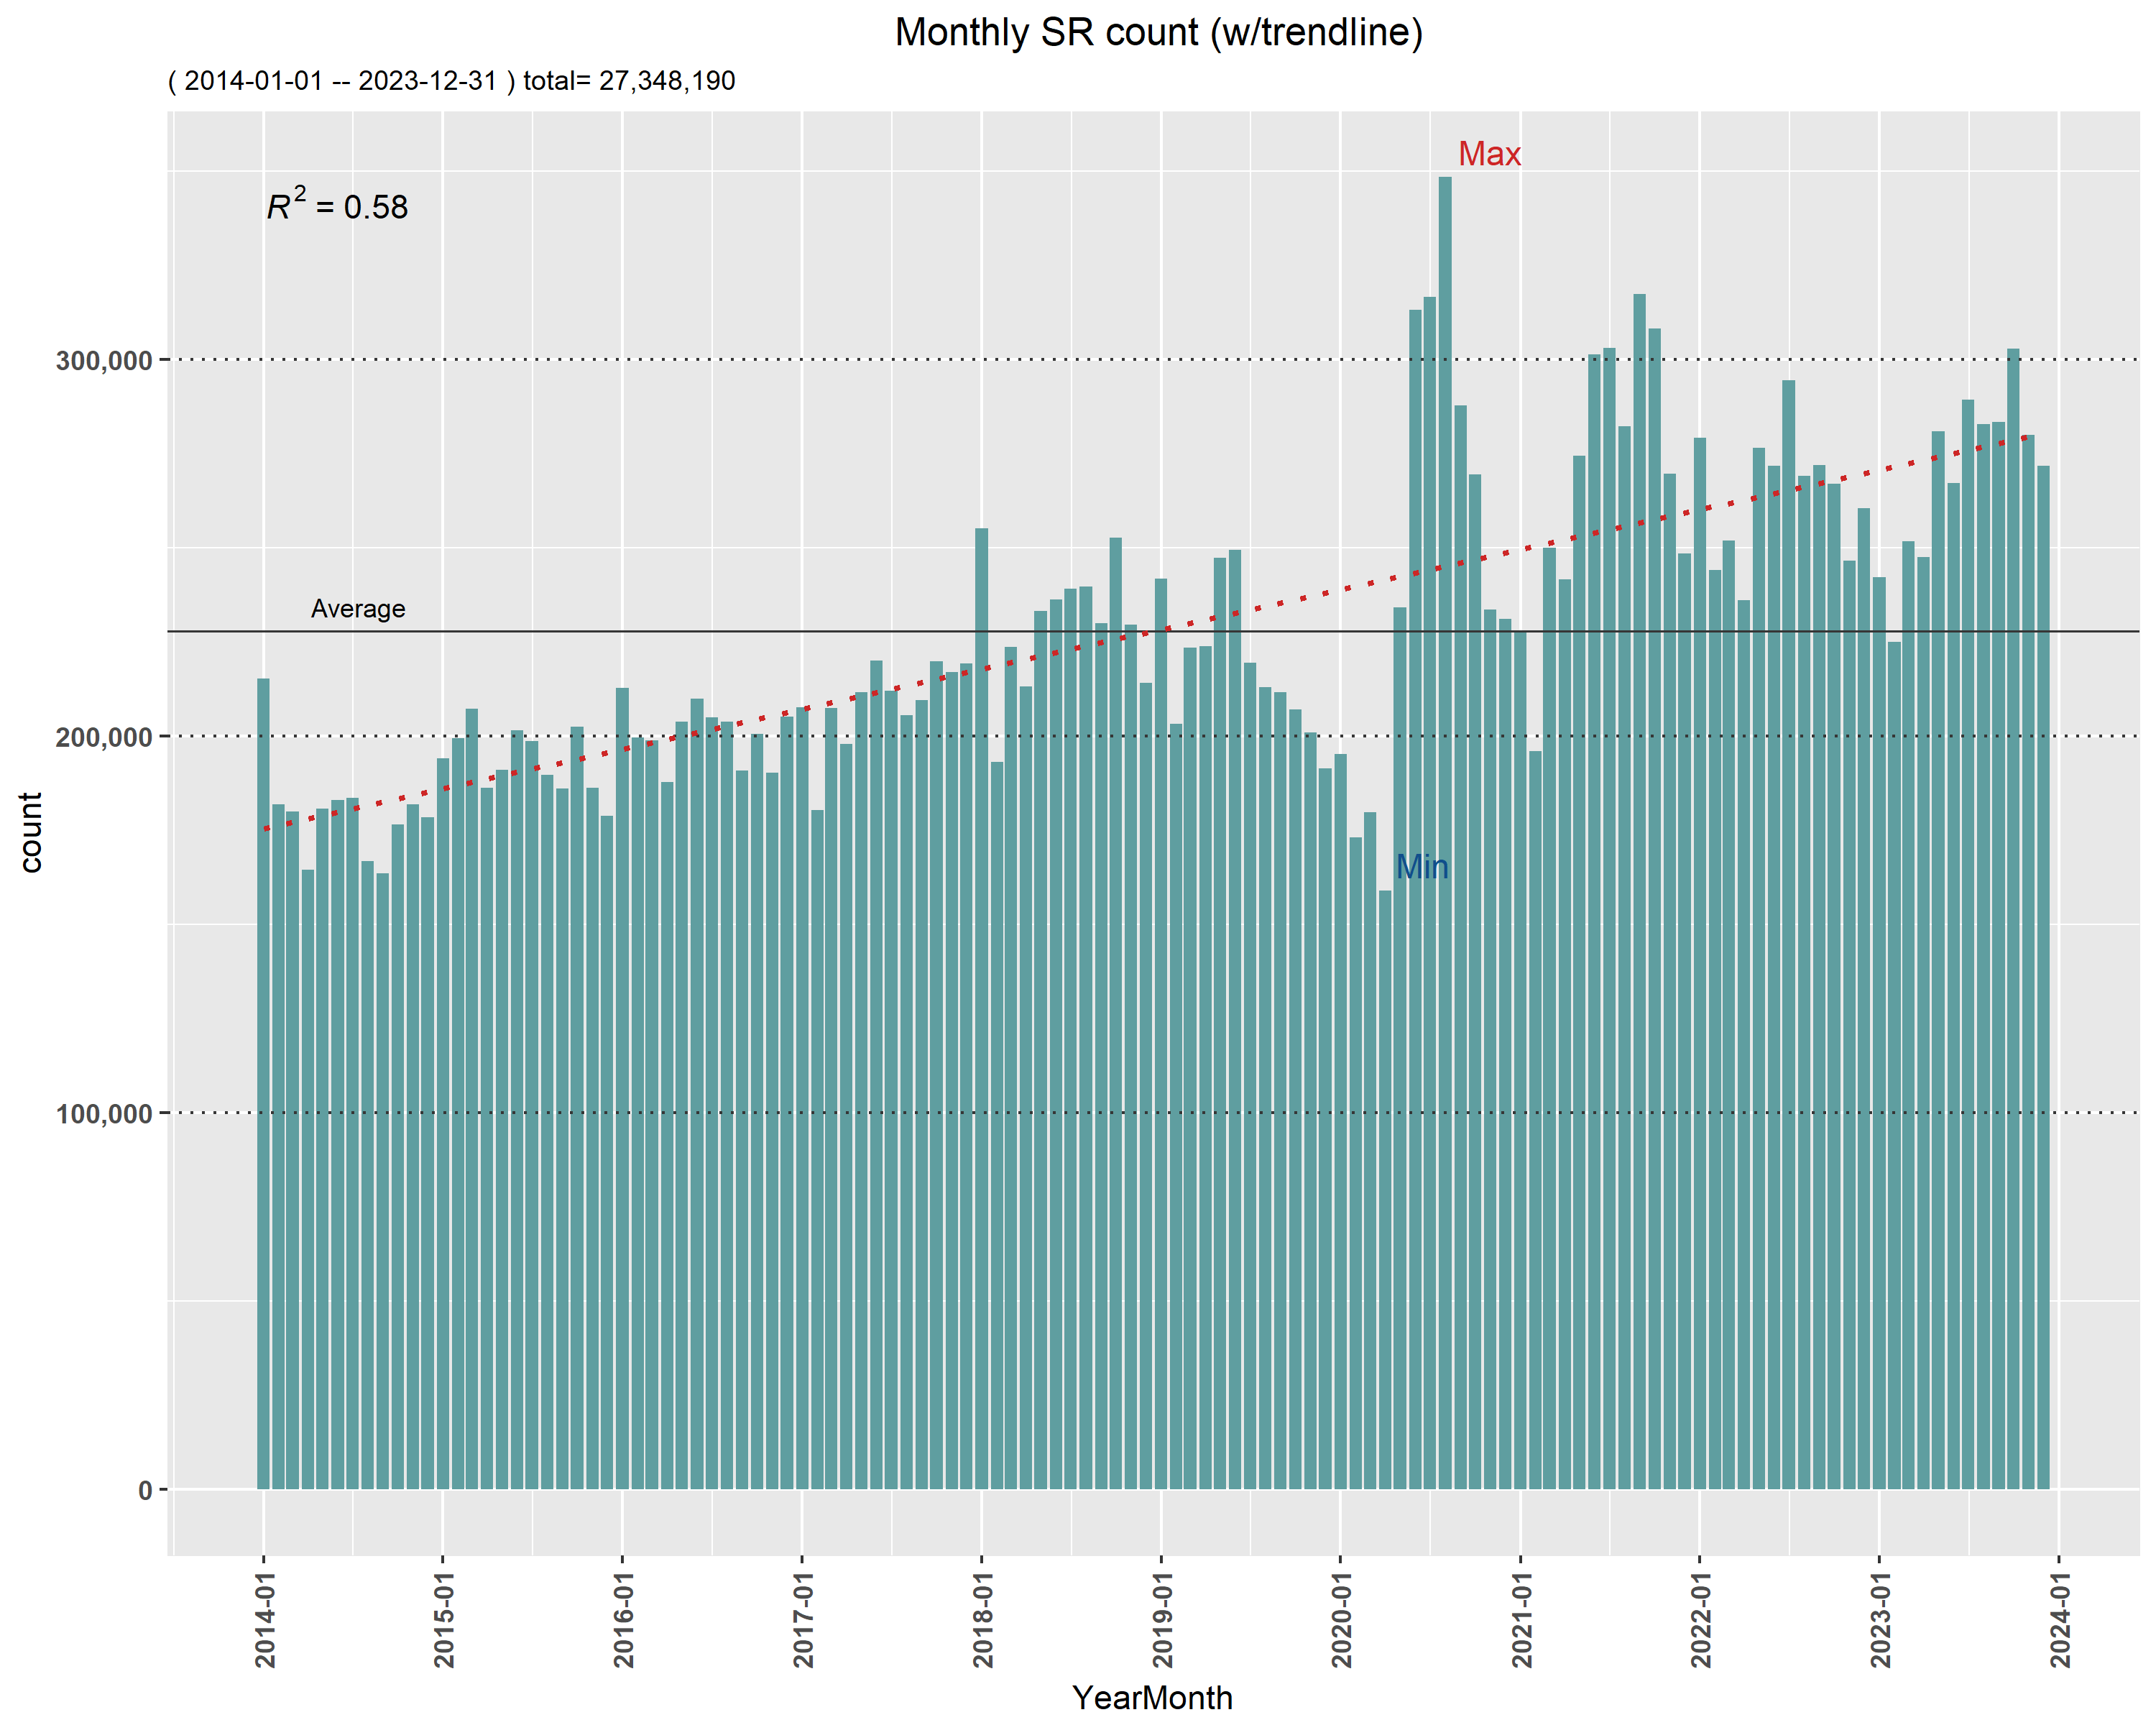
\includegraphics[width=\textwidth]{Monthly.png}
  \caption{Monthly SR counts over 10-year period}
  \label{fig:monthly-counts}
\end{figure}

A quick look at the corresponding  daily tend over a 5-year period (2019-2023) shows both significant spikes
and significant dips; a noisy graph. While the spikes on 2020-08-04 (24,415 SRs) and 2020-08-05 (19,560 SRs) are certainly COVID related, we were unable to 
ascertain any reason for the significant spike on Saturday, 2023-09-29 when 7,962 SRs were created.

\begin{figure}[H]
  \centering
  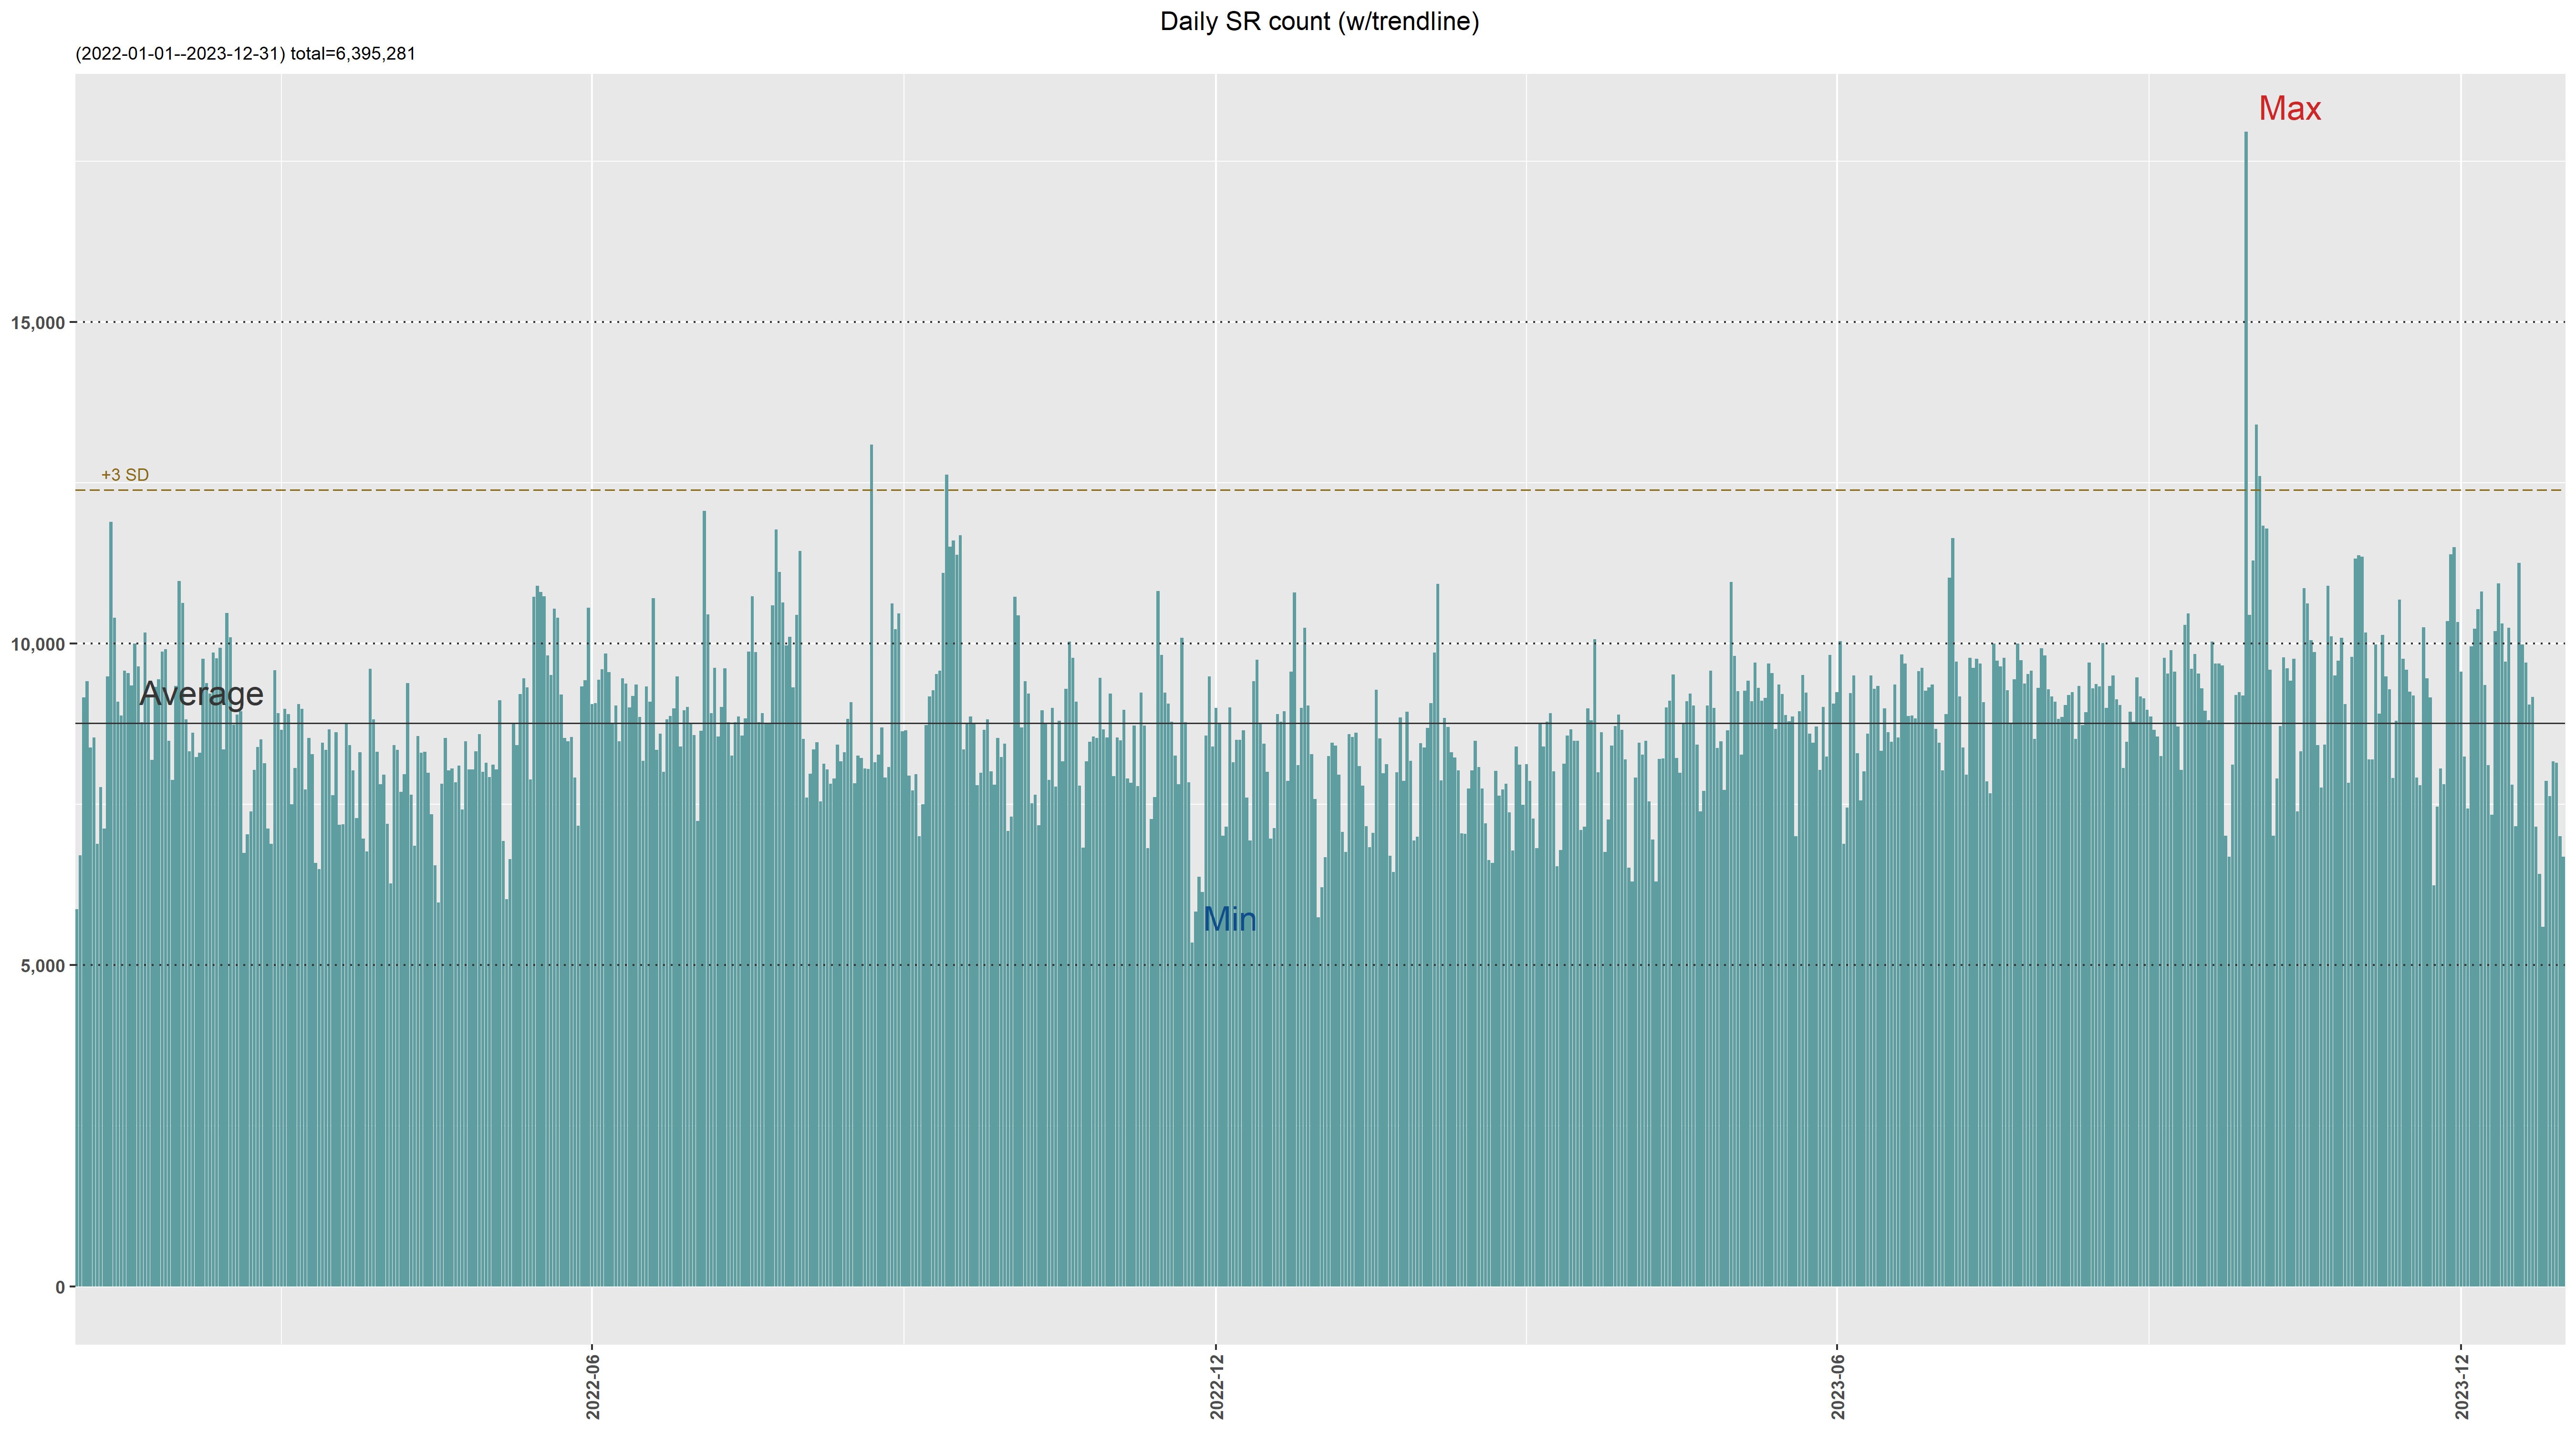
\includegraphics[width=\textwidth]{Daily.png}
  \caption{Daily SR counts over 5-year period}
  \label{fig:daily-counts}
\end{figure}

Seasonal trends are also prevalent. The months of November-thru-April are ``below average'' months, while the months May-thru-October are ``above average''. 
This seasonal trend is observed throughout the 10-year period.

\begin{figure}[H]
  \centering
  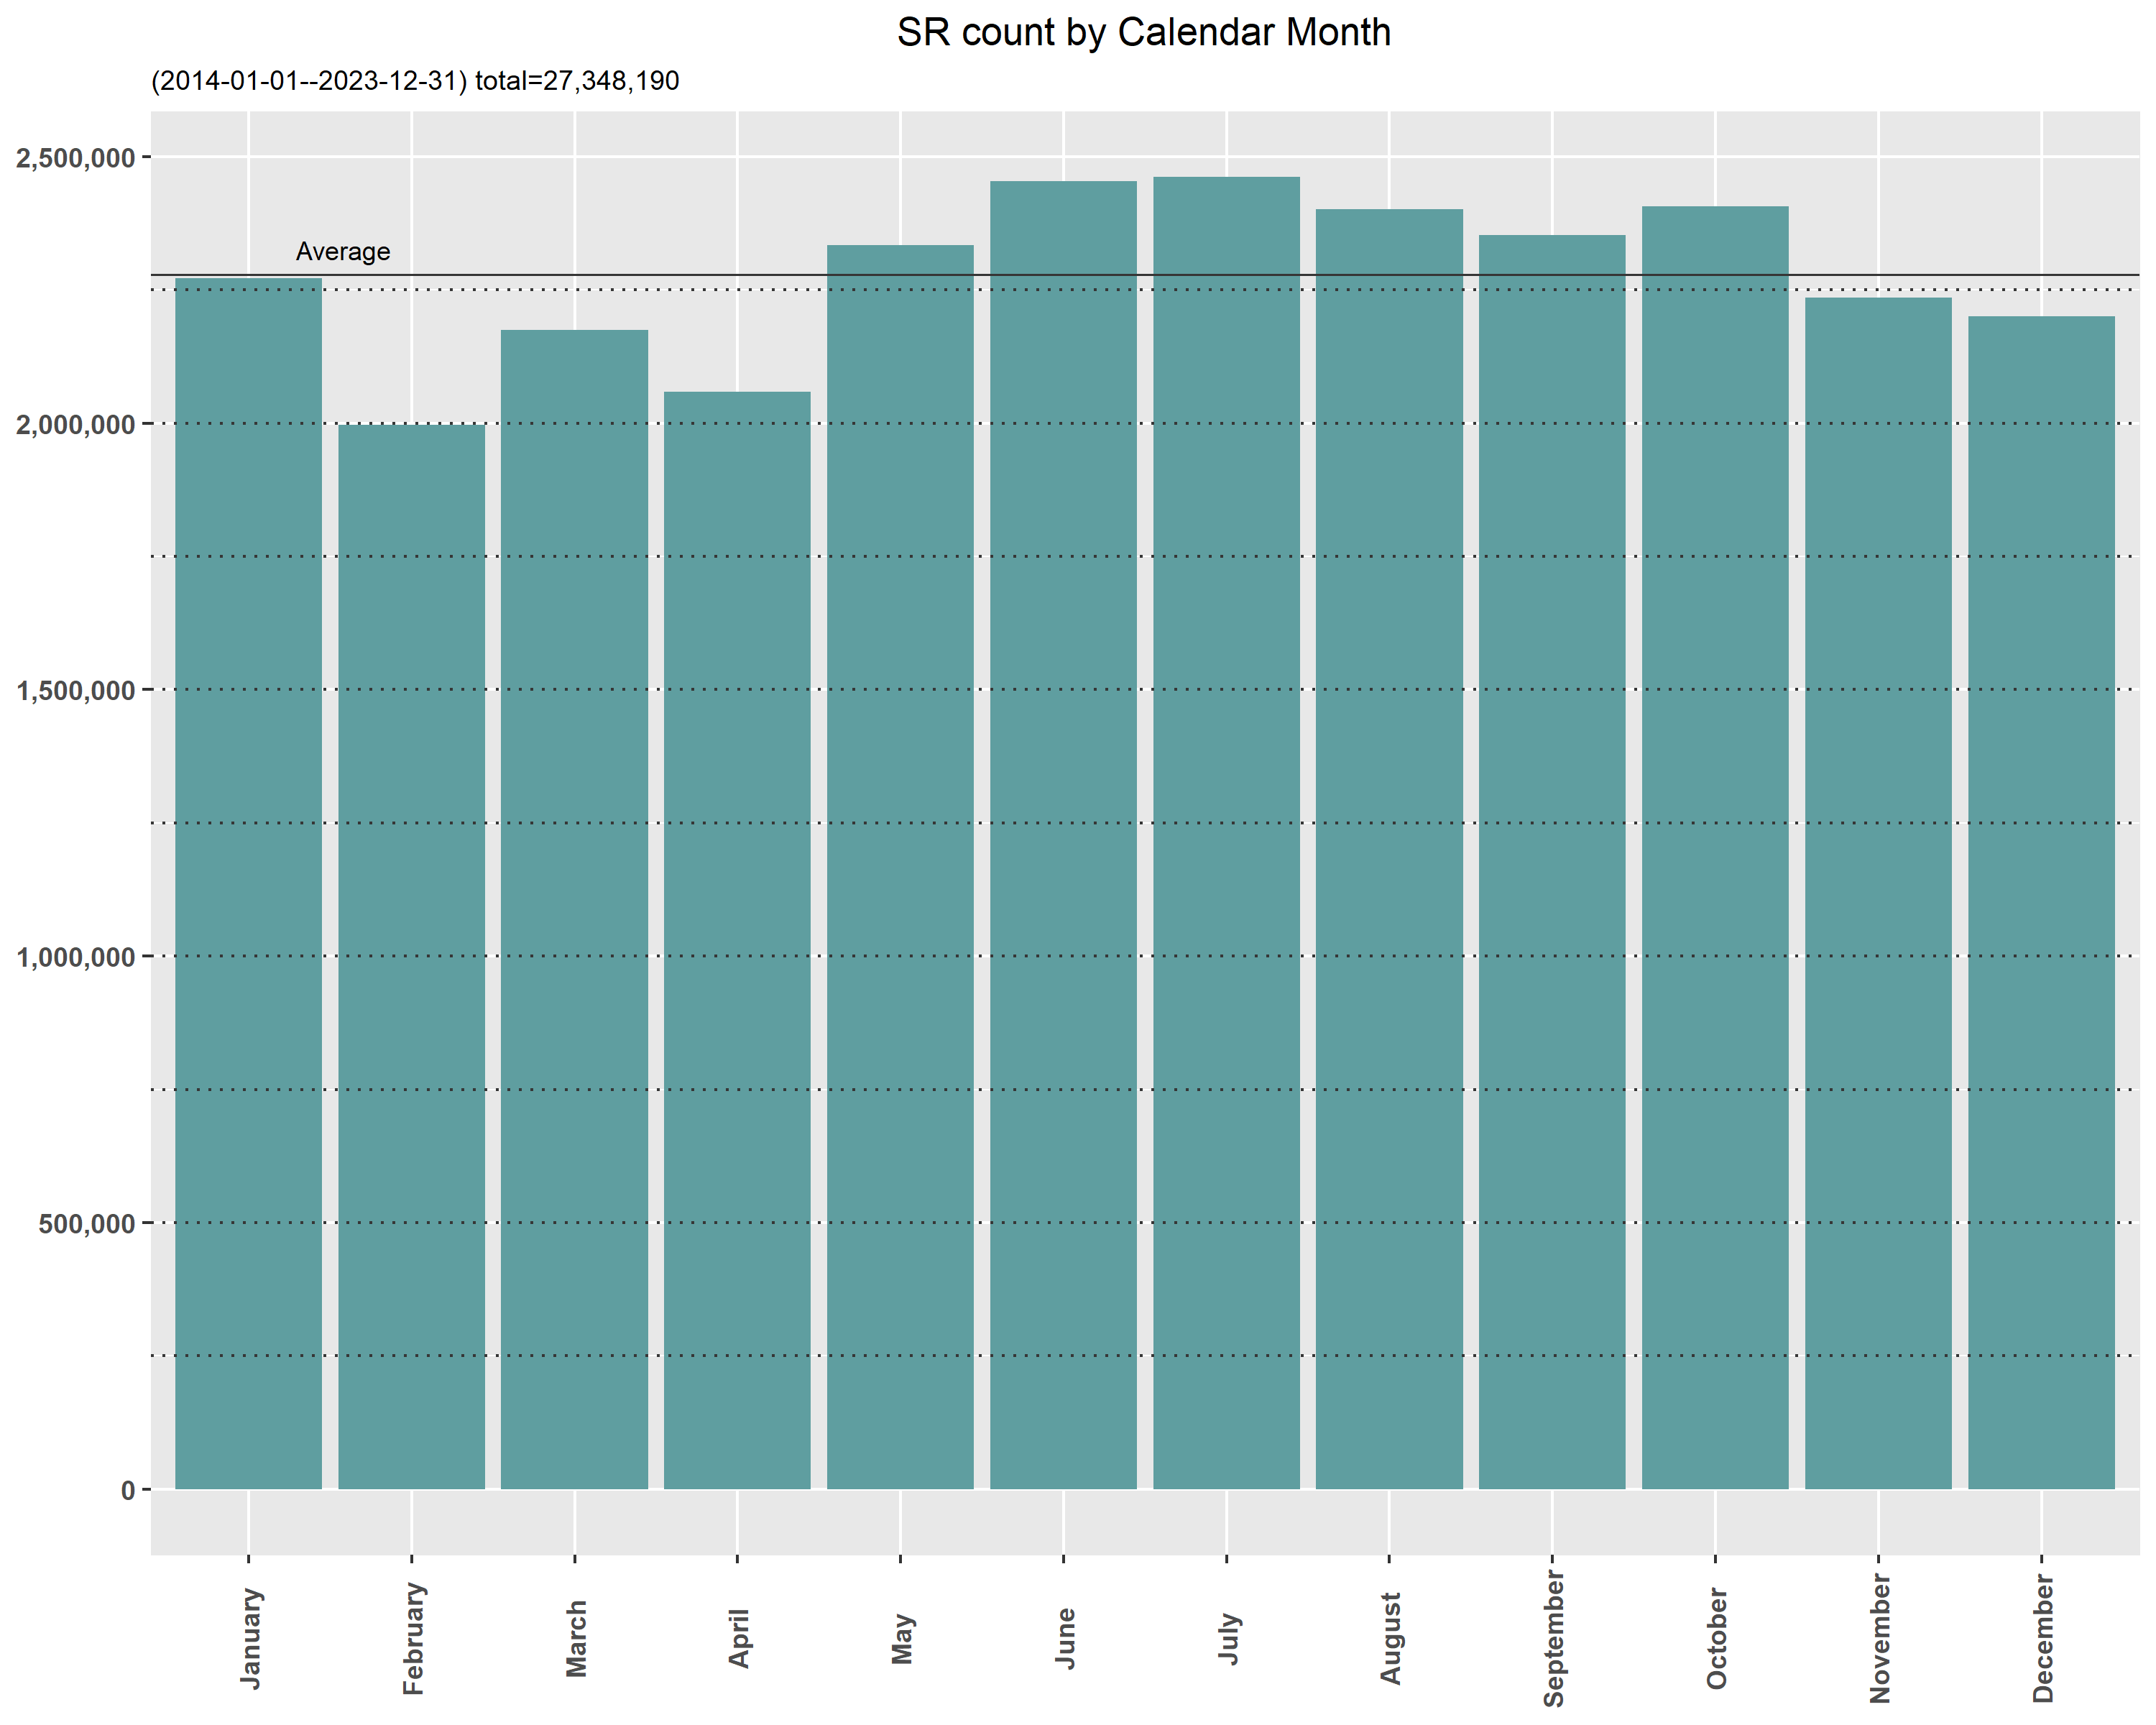
\includegraphics[width=\textwidth]{Calendar-Month.png}
  \caption{Calendar Month SR counts over a 10-year period}
  \label{fig:calendar-months-counts}
\end{figure}

Of note, the lowest SR counts-per-day occur during the Christmas  holiday period encompassing fully 5 of the Bottom 10 SR counts-per-day. The summer months and early
fall months make up all of the Bottom 10 SR counts-per-day. As noted, the all-time daily high for SRs occurred on Tuesday, 2020-08-04 while the 10-year
low count occurs on Christmas Day in 2016, a Sunday. Note also that the difference between the peak day (24,415) and the minimum day (2965) varies
by a factor of 8X, and well exceeds the average daily count of 7489; all of which creates a challenging  system capacity and performance issue.

\begin{table}[H]
    \centering
    \small
    \begin{tabular}{@{}lll|lll@{}}
        \toprule
        \multicolumn{3}{c|}{Top 10 Days} & \multicolumn{3}{c}{Bottom 10 Days} \\
        \cmidrule(r){1-3} \cmidrule(l){4-6}
        Date & Count & Rank & Date & Count & Rank \\
        \midrule
        2020-08-04 & 24415 & 1 & 2014-12-25 & 2965 & 1 \\
        2020-08-05 & 19560 & 2 & 2015-12-25 & 3247 & 2 \\
        2023-09-29 & 17962 & 3 & 2014-04-20 & 3287 & 3 \\
        2020-07-05 & 16916 & 4 & 2015-12-26 & 3405 & 4 \\
        2020-06-21 & 15883 & 5 & 2016-11-06 & 3419 & 5 \\
        2020-06-20 & 15825 & 6 & 2014-07-04 & 3455 & 6 \\
        2020-07-04 & 15794 & 7 & 2014-12-27 & 3534 & 7 \\
        2021-09-02 & 15205 & 8 & 2014-09-14 & 3563 & 8 \\
        2020-06-28 & 14057 & 9 & 2014-02-02 & 3565 & 9 \\
        2021-10-28 & 13575 & 10 & 2016-12-25 & 3587 & 10 \\
        \bottomrule
    \end{tabular}
    \caption{Top 10 and Bottom 10 Days}
    \label{tab:combined_counts}
\end{table}

And although the highest number of SRs occur in July and the lowest in February,
when the \#-of-SRs-per-day metric is computed by adjusting for the differing number of days for each month -- the
busiest month is shown to be June (followed by July and September). Similarly the quietest months are April, March, and 
February. In general, the winter months see fewer SRs while the summer months show 
an increase in activity.

\begin{table}[H]
    \centering
    \small
    \begin{tabular}{lS[table-format=7.0]S[table-format=6.0]} % 'l' for left-aligned, 'S' for siunitx number alignment
        \toprule
        \textbf{Month}     & \textbf{Count}   & \textbf{Count per Day} \\ 
        \midrule
        June  & 2454156 & 81805 \\ 
        July  & 2461525 & 79404 \\ 
        September & 2352822 & 78427 \\ 
        October & 2407238 & 77653 \\ 
        August & 2401731 & 77475 \\ 
        May  & 2334466 & 75305 \\ 
        November  & 2236037 & 74535 \\ 
        January   & 2271524 & 73275 \\ 
        December  & 2199765 & 70960 \\ 
        February  & 1996408 & 70795 \\ 
        March & 2174349 & 70140 \\ 
        April  & 2058169 & 68606 \\ 
       \bottomrule
    \end{tabular}
    \caption{Monthly counts ordered by count-per-day}
    \label{tab:monthly_counts}
\end{table}

\FloatBarrier % Ensure all floats before this point are processed before moving on

Two important fields in this analysis effort are the responsible NYC Agency, and the type of complaint.
Given both the size of the City of New York government, it's necessary to identify the responsible Agency as well as the type of complaint in order to 
clarify the responsible party and assist in troubleshooting discrepancies.

When we discovered a data error, we typically observe two trends; either a single (or a few) Agencies are responsible (such as Dept of Transportation), or it is a system-wide issue that follows the general distribution
of  Service Requests (SRs) across the system. Thus we can often identify if it is an Agency specific problem, or a systemic effect affecting all Agencies.

Although the 311 SRs involve 16 different agencies, there are the ``big six'' Agencies that comprise
90\% of the complaints. These six are (in order of \% of complaints):  

\begin{itemize}
	\item New York Police Department (NYPD)
	\item Housing Preservation \& Development (HPD
	\item New York City Department of Sanitation (DSNY)
	\item Department of Transportation (DOT)
	\item Department of Environmental Protection (DEP)
	\item Department of Parks \& Recreation (DPR)
\end{itemize}

\begin{figure}[H]
  \centering
	  \includegraphics[width=\textwidth]{SRs\_by\_Agency.png}
	  \caption{SR counts by Agency and Cumulative Percentage}
	  
\end{figure}

Note the distribution of the complaint\_type; it is heavily skewed to a few select complaints with an exceptionally long tail.
This graph shows the top 20 complaint\_type(s) out of a total of 220.

\begin{figure}[H]
  \centering
	  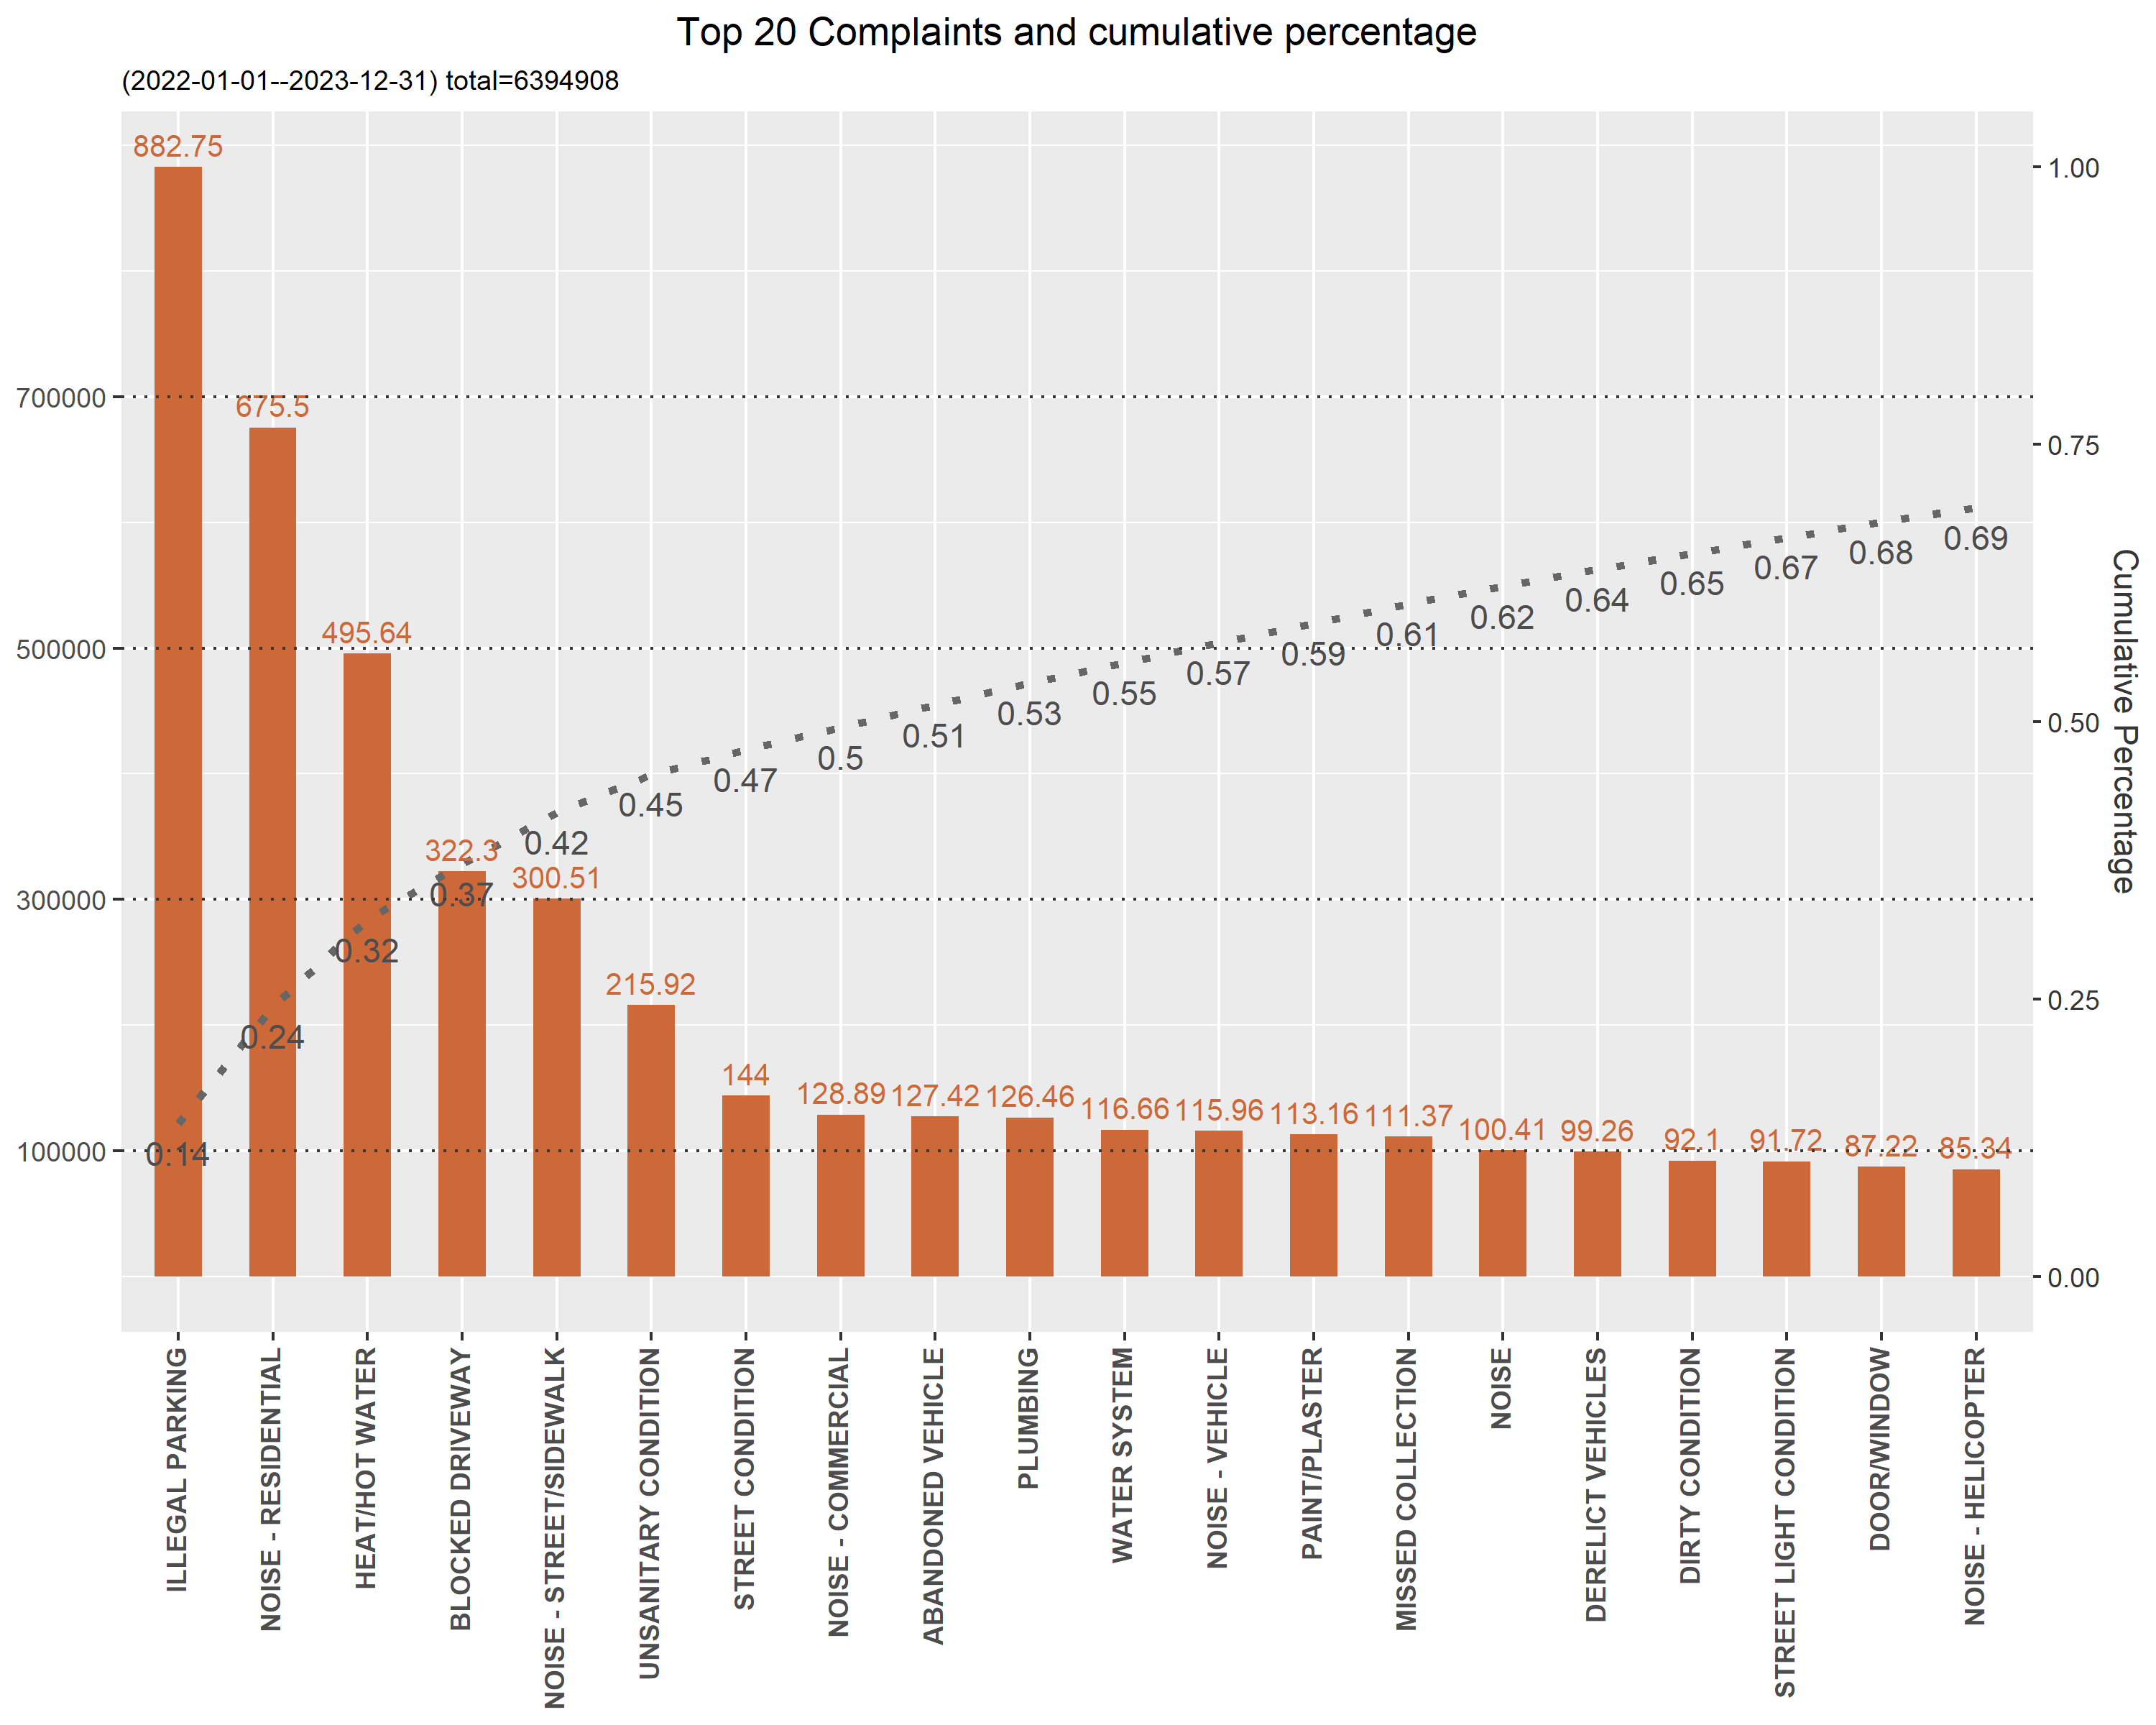
\includegraphics[width=\textwidth]{SRs_by_Complaint_Type.png}
	  \caption{Top 20 SR complaint\_type and Cumulative Percentage}
	  \label{fig:SR_complaints}
\end{figure}

The top 20 complaints contain several of the eight different types of ``Noise'' complaints (Residential, Commercial, Street, Helicopter, etc.). These Noise-related
complaints total 1.435 million in the 2022-2023 dataset, a full 22\% of all complaint types, which is the most frequently occurring type. (Note: Ilegal Parking is second, followed by Heat/Hot Water.) Noise complaints are also handled by NYPD, as is Illegal Parking and Blocked Driveway complaints, which contributes
significantly to the top ranking of the NYPD as the responsible Agency.

\begin{table}[H]
    \centering
    \footnotesize
    \begin{tabular}{lS[table-format=7]S[table-format=2.2]l} % 'l' for left-aligned, 'S' for siunitx number alignment
        \toprule
        \textbf{complaint\_type} & \textbf{Count} & \textbf{Percentage} & \textbf{Agency} \\ 
        \midrule
        NOISE - RESIDENTIAL        & 675502 & 10.56 & NYPD  \\ 
        NOISE - STREET/SIDEWALK    & 300507 &  4.70 & NYPD  \\ 
        NOISE - COMMERCIAL         & 128892 &  2.02 & NYPD  \\ 
        NOISE - VEHICLE            & 115956 &  1.81 & NYPD  \\ 
        NOISE                      & 100413 &  1.57 & DEP   \\ 
        NOISE - HELICOPTER         &  85345 &  1.33 & EDC   \\ 
        NOISE - PARK               &  16620 &  0.26 & NYPD  \\ 
        NOISE - HOUSE OF WORSHIP   &   2757 &  0.04 & NYPD  \\ 
        \bottomrule
    \end{tabular}
    \caption{Noise-related complaints\_type(s) by count with Agency}
    \label{tab:noisecomplaints}
\end{table}

There are also some  curious and unusual Service Requests in the 311 data: 
tanning, tattooing, trans fat, unsanitary pigeon condition, illegal animal kept as pet, harboring bees/wasps, and the author's favorite
radioactive material. New Yorkers certainly live interesting lives. 

The NYC HPD handles about 49\% of what NYPD handles. For  non-NYC readers, 
HPD is the City agency that manages the 177,569 NYC public housing units as well as monitoring
all rental and leased apartment units. HPD collectively serves 528,105 people, a population larger than Atlanta or Miami. 
Hence the large number of Heat/Hot Water and Unsanitary complaints handled by HPD. 



\section{Data Cleansing Issues} \label{sec:issues}

What is data cleansing?  Wikipedia \href{https://en.wikipedia.org/wiki/Data_cleansing}{Data Cleansing} offers a good definition. 

``Data cleansing or data cleaning is the process of detecting and correcting (or removing) corrupt or inaccurate records from a record set, 
table, or database and refers to identifying incomplete, incorrect, inaccurate or irrelevant parts of the data 
and then replacing, modifying, or deleting the dirty or coarse data.''

Many quality criteria are required in order to process high-quality data. These include:

\begin{itemize}
	\item Data validation - this effort can span a number of criteria
	\begin{itemize}
		\item Mandatory fields: Certain data fields cannot be empty.
		\item Data-types: Certain fields must be of the correct type, e.g. numeric, character, date, 5 numeric digits, etc. Typically these are identified in a Data Dictionary.
		\item Domain adherence:  Many data fields must adhere to a specific domain of values, e.g. statuses, state names, zip codes, gender. This includes data
		fields that are restricted to certain ranges, such as longitudes and latitudes.
	\end{itemize}   
	\item Structural errors to include naming conventions, extra fields not in the Data Dictionary, or inconsistent data entry.
	For example intermixing blanks, spaces, NA, N/A, and <NA> all to indicate the absence of data.
	\item Redundant, unnecessary, or irrelevant fields
	\item Logical inconsistencies such as related fields that violate the nature of that relationship, e.g. a ``due date'' that is before the ``created date''
	\item Data standardization. Often free-form entry fields can suffer from inconsistent data structures. Efforts to standardize these fields can greatly assist analysis.
	\item Accuracy and precision, which of course are not the same thing 
\end{itemize}

This analysis effort is to identify the presence of such errors; not to correct them. That effort would be undertaken only after an investigation as to the why
and how such errors came about, and a discussion as to whether or not it is even an ``error''. Typically this requires discussions with subject matter experts (SMEs)
 and liaison within the various NYC Agency open data coordinators who can help identify the underlying cause for the error.
 For example, an invalid date field that is provided to the NYC Open Data data lake via an Agency integration could
be the result of selecting the wrong field from the source Agency's system, e.g. due\_date instead of closed\_date. In other cases, without a subject matter
expert, it is not possible to actually determine if the data is inaccurate or not. There are many empty values in the taxi\_company\_borough field. Are those
entries missing or does the entry in that field only apply to a very small number of complaint\_type(s) or circumstances. Only a SME
from the Taxi \& Limo Commission (TLC) can provide that answer. The R code used here to analyze the 311 Service Request dataset identifies
both obvious inaccuracies as well as potential errors requiring further investigation. It is not a conclusive list of errors, but rather mostly identifies
``a place to look'' for further evaluation and potential action.

This paper will focus on a set of specific data cleansing areas:

\begin{itemize}
	\item Examining structural issues within the data
	\item Validating data type correctness
	\item Identifying missing, blank, or N/A data
	\item Identifying invalid values
	\item Exposing logical inconsistencies \& inconsistent or unusual patterns in the data
	\item Accuracy and precision issues
	\item Identifying potential redundant or irrelevant data  
\end{itemize}



\section{Structural Issues}\label{sec:structural}

Structural issues in the context of data cleansing refers to issues related to the how data is organized, formatted, or structured within a dataset. Structural issues 
can make it difficult to analyze the data effectively. Some common structural concerns in this 311 SR 2022-2023 dataset include:

\begin{itemize}
	\item Data structure (data fields, columns, formats, data types, etc.) not corresponding to the Data Dictionary
	\item Verification of correct data types (numeric, character, geospactial, dates, etc.)
	\item Embedded or combined values: data elements that contain multiple pieces of information 
\end{itemize}

Here are some characteristics of the 311 SR data set:

\begin{itemize}
	\item There are 47 columns of data for each row, exportable as a CSV file.
	\item There are four date fields (created, closed, updated, due).
	\item There are three borough fields; two of which we believe to be duplicates.
	\item Two zip code fields, but not duplicates
	\item Seven street fields; one pair of which we believe to be duplicates
	\item Agency name and Agency abbreviation
	\item Two Police Precinct fields; not duplicates
	\item In addition to street/city, there are three other location fields: lat/long, NY State plane, and Block \#
	\item incident\_address and street\_name, e.g. incident\_address, 25 Grymes Hill Road and street\_name (Grymes Hill Road)
	\item One free-form text field, resolution\_description, which supports 934 characters of input, including commas and special characters
\end{itemize}


\textbf{Issue: Fields not in the Data Dictionary} The 311 SR \href{https://data.cityofnewyork.us/api/views/erm2-nwe9/files/b372b884-f86a-453b-ba16-1fe06ce9d212?download=true&filename=311_ServiceRequest_2010-Present_DataDictionary_Updated_2023.xlsx}{Data Dictionary}
 identifies 41 data columns (fields) along with related information for each column. 
 However, when you download the data or explore it via the online portal, you immediately note that there are 47 columns (fields).
 he additional six fields are not addressed in the Data Dictionary, but do and show up on the Column Manager widget
 as ``@computed\_region\_xxxx\_xxxx''. To some extent one can infer what the these @computed\_fields are, but it is not possible to know
for certain. These six fields are:

\begin{itemize}
	\item zip\_codes
	\item community\_districts
	\item borough\_boundaries
	\item city\_council\_districts
	\item police\_precincts
	\item police\_precinct 
\end{itemize}	

Here is a screenshot of the NYC Open Data Portal ``Column Manager'' page showing those columns:

\begin{figure}[H]
  \centering
	  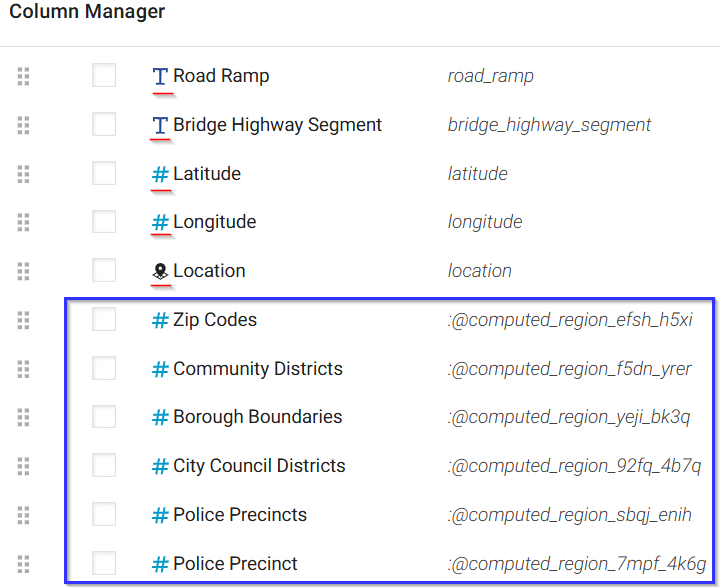
\includegraphics[scale = 0.65]{computed_columns_screenshot.png}
	  \caption{Screenshot of data portal showing the ``@computed'' columns}
	  \label{fig:computed-columns}
\end{figure}

This, of course, raises several questions:

\begin{itemize}
	\item How are these fields computed? Using what source data? Using what computational method?
	\item How can these fields be verified or cross-checked?
	\item Why are there two fields that appear redundant ``police\_precinct' and ``police\_precincts''? Are these redundant?
	\item What are ``borough boundaries''? They appear to be borough names. Why are they referred to as ``boundaries''?
	\item What are ``community districts''? Is this the same as the ``community\_board(s)'' that are part of the NYC government?
	\item Why are not these fields included in the official 311 SR Data Dictionary?
	\item Can these fields be reliably used for analytical purposes? 
\end{itemize}	

The last bullet point is the key here. Are these fields reliable and accurate, and can they be used for subsequent analysis? Unfortunately,
as of this date, those questions have not been fully addressed by the  NYC Open Data Team. This paper will further address that issue by
exploring the accuracy, validity, and candidacy for subsequent analytical usage.
	
	
	
\section{Validating data types}\label{sec:datatypes}
Fortunately, both the Data Dictionary and the portal column manager do a good job of indicating the data type.
As indicated by the red underline in Figure \ref{fig:computed-columns}, there is a small icon next to the field name 
which indicates the data type of the field. The stylized capital ``T'' indicates ``text'', the ``\#'' sign indicates 
``numeric'', a calendar icon indicates a ``date'' field, and the pin on a map symbol indicates a ``geospatial'' field. 
	
The following fields were checked for their specified data types:
	
\begin{itemize}
	\item created\_date, closed\_date, due\_date, and resolution\_action\_updated\_date: All are all in proper date format.
	\item zip\_codes and incident\_zip: All are 5 numeric digits except for 2 non-numeric entries for incident\_zip (``na'' and ``N/A'').
	\item x\_coordinate\_state\_plane \&  y\_coordinate\_state\_plane (a NY State geo-location system): All are all numeric.
	\item latitude \& longitude: Both are numeric.
	\item community\_districts, borough\_boundaries, city\_council\_district, police\_precinct, and police\_precincts: All are numeric.
	\item Free-form text fields that contain a ``,'' (e.g. incident\_address \& resolution\_description) are properly enclosed in quotation marks.
\end{itemize}	

All data fields were subjected to a test of ``correctness'' according to their ``type'' as specified
in the Data Dictionary. Of the nearly 300 million data fields to check (6.5 million rows, 47 fields per row), there were only two values that failed to test the
test for appropriate data type; those being two text entries in the incident\_zip field (``na'', and ``N/A''). All date fields were dates. All numbers were numeric.
All text fields were character. Data typing appears to not be an issue with this dataset.

 

\section{Blank \& N/A data}\label{sec:blanks}

Understanding the absence of data by field is an important factor when undertaking analysis. For example, if you wanted to see if the SRs were
closed before or after their due\_date, you would be challenged as 99.57\% of the due\_date field is blank. (Although with such a large dataset
that still leaves 24,411 values, all of which are ``N/A'. Which calls into question...are these missing values, or is the concept of a
due\_date simply not applicable for the vast majority of SRs?

When counting the various fields for blank or N/A values, the fields appear to divide into three groups: \textbf{Mostly Empty}, \textbf{Partially Empty}, 
and \textbf{Few/None Empty}. he Mostly Empty category ranges from 93-99.9\% blank. It includes such fields as taxi\_company due\_date, pickup\_location, and landmark. The Partially 
Empty includes such fields as location\_type, borough, and cross\_street. And the Few/None Empty includes created\_date, complaint\_type, agency, and status.
In some cases it may make sense to inquiry as to why some fields are frequently blank. Is the data difficult to capture? Does it pertain to only a small set
of complaint\_type(s) or Agencies? And if the data is truly that sparse, does it even make sense to collect it? Is it legacy data? For example, one would expect that every complaint\_type
that has a geographical component, such as an address, would also have a corresponding police\_precinct, community\_board, and community\_district since these
are all-inclusive throughout the five Boroughs of NYC. Addtionally, that it would have a lat/long. And generally that is the case, but these fields do have small number, but nonetheless significant, 
of empty entries. 

During the analysis, it was determined that the following fields are mandatory, and any row missing these fields should be removed from the dataset (which fortunately
very rarely occurred): created\_date, agency, complaint\_type, and unique\_key. The absence of any one of these four fields prohibits further analysis  as currently conducted. Again,
it is very rare occurrence, happening only 1-2 times in 6.4 million records. Here is a breakdown of bank and N/A entries by field.

\begin{table}[ht]
\centering
\resizebox{0.8\linewidth}{!}{%
\scriptsize
\begin{tabular}{lrrrl}
	\toprule
	\textbf{Field} & \textbf{Total Empty} & \textbf{Percent Empty} & \textbf{N/A Count} \\
	\midrule
		taxi\_company\_borough & 6391341 & 99.94 & 0 \\
		road\_ramp & 6379080 & 99.75 & 0 \\
		vehicle\_type & 6376266 & 99.71 & 0 \\
		due\_date & 6370497 & 99.62 & 6370497 \\
		bridge\_highway\_direction & 6367626 & 99.57 & 0 \\
		bridge\_highway\_name & 6340197 & 99.14 & 0 \\
		bridge\_highway\_segment & 6340190 & 99.14 & 0 \\
		taxi\_pick\_up\_location & 6329954 & 98.98 & 0 \\
		facility\_type & 5966588 & 93.30 & 0 \\
		landmark & 2635736 & 41.22 & 0 \\
		intersection\_street\_1 & 2143847 & 33.52 & 0 \\
		intersection\_street\_2 & 2140707 & 33.48 & 0 \\
		cross\_street\_1 & 1846594 & 28.88 & 0 \\
		cross\_street\_2 & 1846008 & 28.87 & 0 \\
		location\_type & 798775 & 12.49 & 0 \\
		bbl & 768109 & 12.01 & 0 \\
		city & 332086 & 5.19 & 0 \\
		street\_name & 280463 & 4.39 & 0 \\
		incident\_address & 280268 & 4.38 & 0 \\
		closed\_date & 248839 & 3.89 & 248839 \\
		resolution\_description & 132333 & 2.07 & 0 \\
		zip\_codes & 123167 & 1.93 & 0 \\
		borough\_boundaries & 101453 & 1.59 & 0 \\
		community\_districts & 101445 & 1.59 & 0 \\
		city\_council\_districts & 101445 & 1.59 & 0 \\
		police\_precincts & 101445 & 1.59 & 0 \\
		police\_precinct & 101416 & 1.59 & 0 \\
		latitude & 99778 & 1.56 & 0 \\
		longitude & 99778 & 1.56 & 0 \\
		location & 99778 & 1.56 & 0 \\
		x\_coordinate\_state\_plane & 99668 & 1.56 & 0 \\
		y\_coordinate\_state\_plane & 98822 & 1.55 & 0 \\
		resolution\_action\_updated\_date & 91399 & 1.43 & 91399 \\
		incident\_zip & 83220 & 1.30 & 2 \\
		descriptor & 74645 & 1.17 & 0 \\
		address\_type & 38655 & 0.60 & 0 \\
		unique\_key & 0 & 0.00 & 0 \\
		agency & 0 & 0.00 & 0 \\
		agency\_name & 0 & 0.00 & 0 \\
		complaint\_type & 0 & 0.00 & 0 \\
		status & 0 & 0.00 & 0 \\
		community\_board & 0 & 0.00 & 0 \\
		borough & 0 & 0.00 & 0 \\
		open\_data\_channel\_type & 0 & 0.00 & 0 \\
		park\_facility\_name & 0 & 0.00 & 0 \\
		park\_borough & 0 & 0.00 & 0 \\
		created\_date & 0 & 0.00 & 0 \\
	\bottomrule
\end{tabular}
}
\caption{Blank and N/A entries by Field}
\end{table}

\FloatBarrier % Ensure all floats before this point are processed before moving on

Here is a graphic depiction of total empty (blank \& N/As) for each fields. You can see the natural grouping into the Most, Some, and Few categories
in the stair-type visualization. 

\begin{figure}[H]
  \centering
	  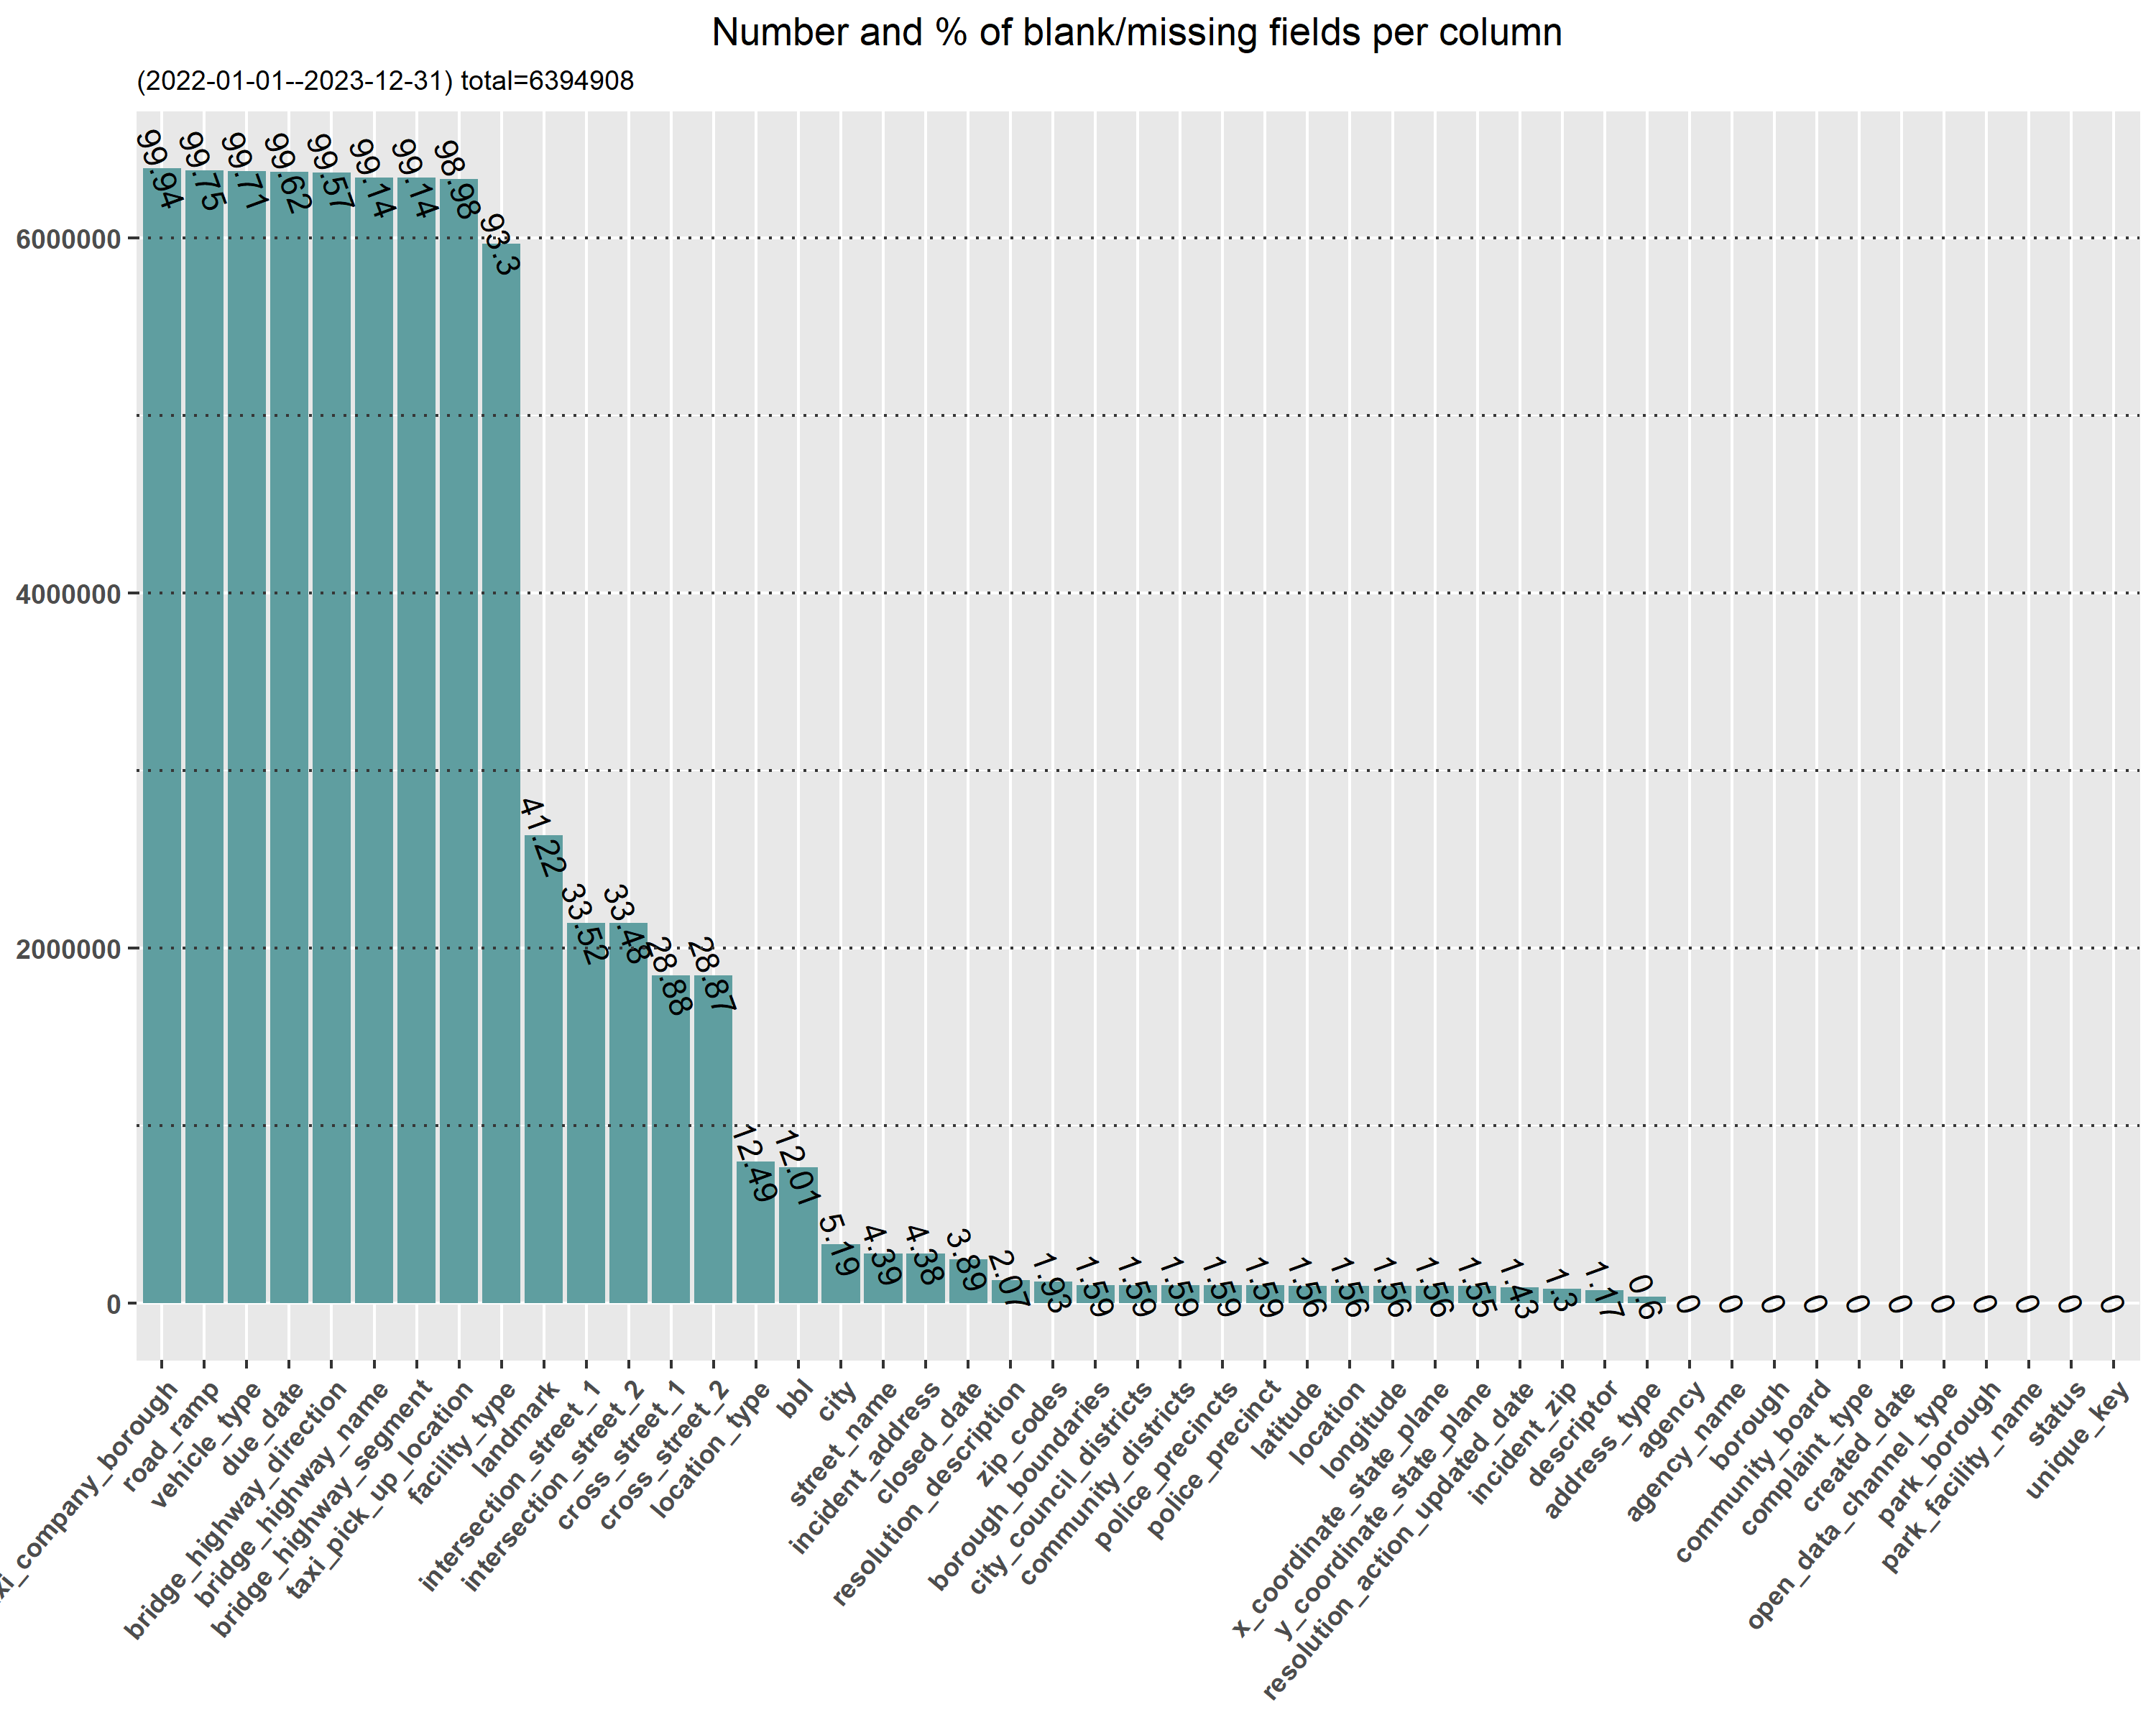
\includegraphics[width=\textwidth]{BlankFields.png}
	  \caption{Number and Percentage of Empty Entries}
	  \label{fig:blank_fields}
\end{figure}



 \section{Validating Data for Acceptable Values}\label{sec:domain}
 While the dataset may have fields populated with data that appears correct, it is necessary to inspect those fields to determine if the data is indeed valid. 
 For example a date field that contains the value ``February 30, 2024'' is clearly not valid. Nor is a latitude of +95 deg north. 
 
 In this study, testing for invalid values revealed several serious issues associated with select fields. Accordingly, an analyst would need to be
extra diligent if using these fields for analysis. In all likelihood, rows with invalid field values would  need to be removed from the
dataset before conduction further analysis. Here are some results.

\begin{itemize}
	\item Latitude and Longitude fields were tested to ensure all fell within the geographic boundaries of the City of New York. All did.
	\item The unique\_key field was in fact unique.
	\item Many fields have a domain of acceptable values. Often these values are determined from common usage or by examining
	larger historical datasets. Unfortunately, these domains of acceptable values are not specified in the Data Dictionary. These fields all tested as
	compliant within their domain of acceptable values as determined by examining a 10-year dataset:
		\begin{itemize}
			\item address\_type
			\item status
			\item borough, borough\_boundaries, \& park\_borough 
			\item data\_channel
			\item vehicle\_type
			\item city\_council\_district
		\end{itemize}
\end{itemize}	

	\subsection{Issues with Zip Codes}
	 Unfortunately some fields proved to be  problematic when comparing the values to a domain of legal values.
	 For example, all zip codes (two fields: zip\_codes and incident\_zip) should be valid as defined by the USPS database
	 which contains 37,946 valid zip codes.
	 
	The computed field zip\_codes proved especially problematic with 58\% (3.6 million) of the field entries being invalid.
	That high number indicates that the computation of this field is highly inaccurate. We recommend
	dropping this field for future analytic efforts.
	
	Furthermore, the field incident\_zip while having only .07\% invalid entries, still is a problem with 4163 such errors.
	As the zip code is a primary measure of many NYC city services, 
	and with a freely available database for which to validate entries, it seems an oversight 
	that any such errors could creep into the 311 system. Some invalid entries can  
	clearly be identified as incorrect just by observation, e.g. 10000, 12345, 11111, etc. 
	
	The breakdown of the invalid entries in the zip\_code, sorted by Agency shows that the distribution by percentage
	almost precisely mirrors the overall breakdown of SRs by Agency as shown in . This indicates a systemic problem, and since the
	zip\_code fields is one of the computed fields, it appears these errors are caused by incorrect computations rather
	than by any Agency mistake.
	
	The  errors in the incident\_zip field are more troubling, even though they are, percentage-wise, small. Here is a graphic 
	illustrating how these errors occur by Agency. Here we can see that the majority of these errors lie in the Dept of Transportation,
	NYPD, Taxi \& Limo Commission (TLC), and the Economic Development Council (EDC) among others. This representation
	does not follow the full SR distribution indicating that these errors are likely generated by an incorrect
	process or application residing at those particular Agencies; it is not a systemic problem.

	\begin{figure}[H]
	  \centering
		  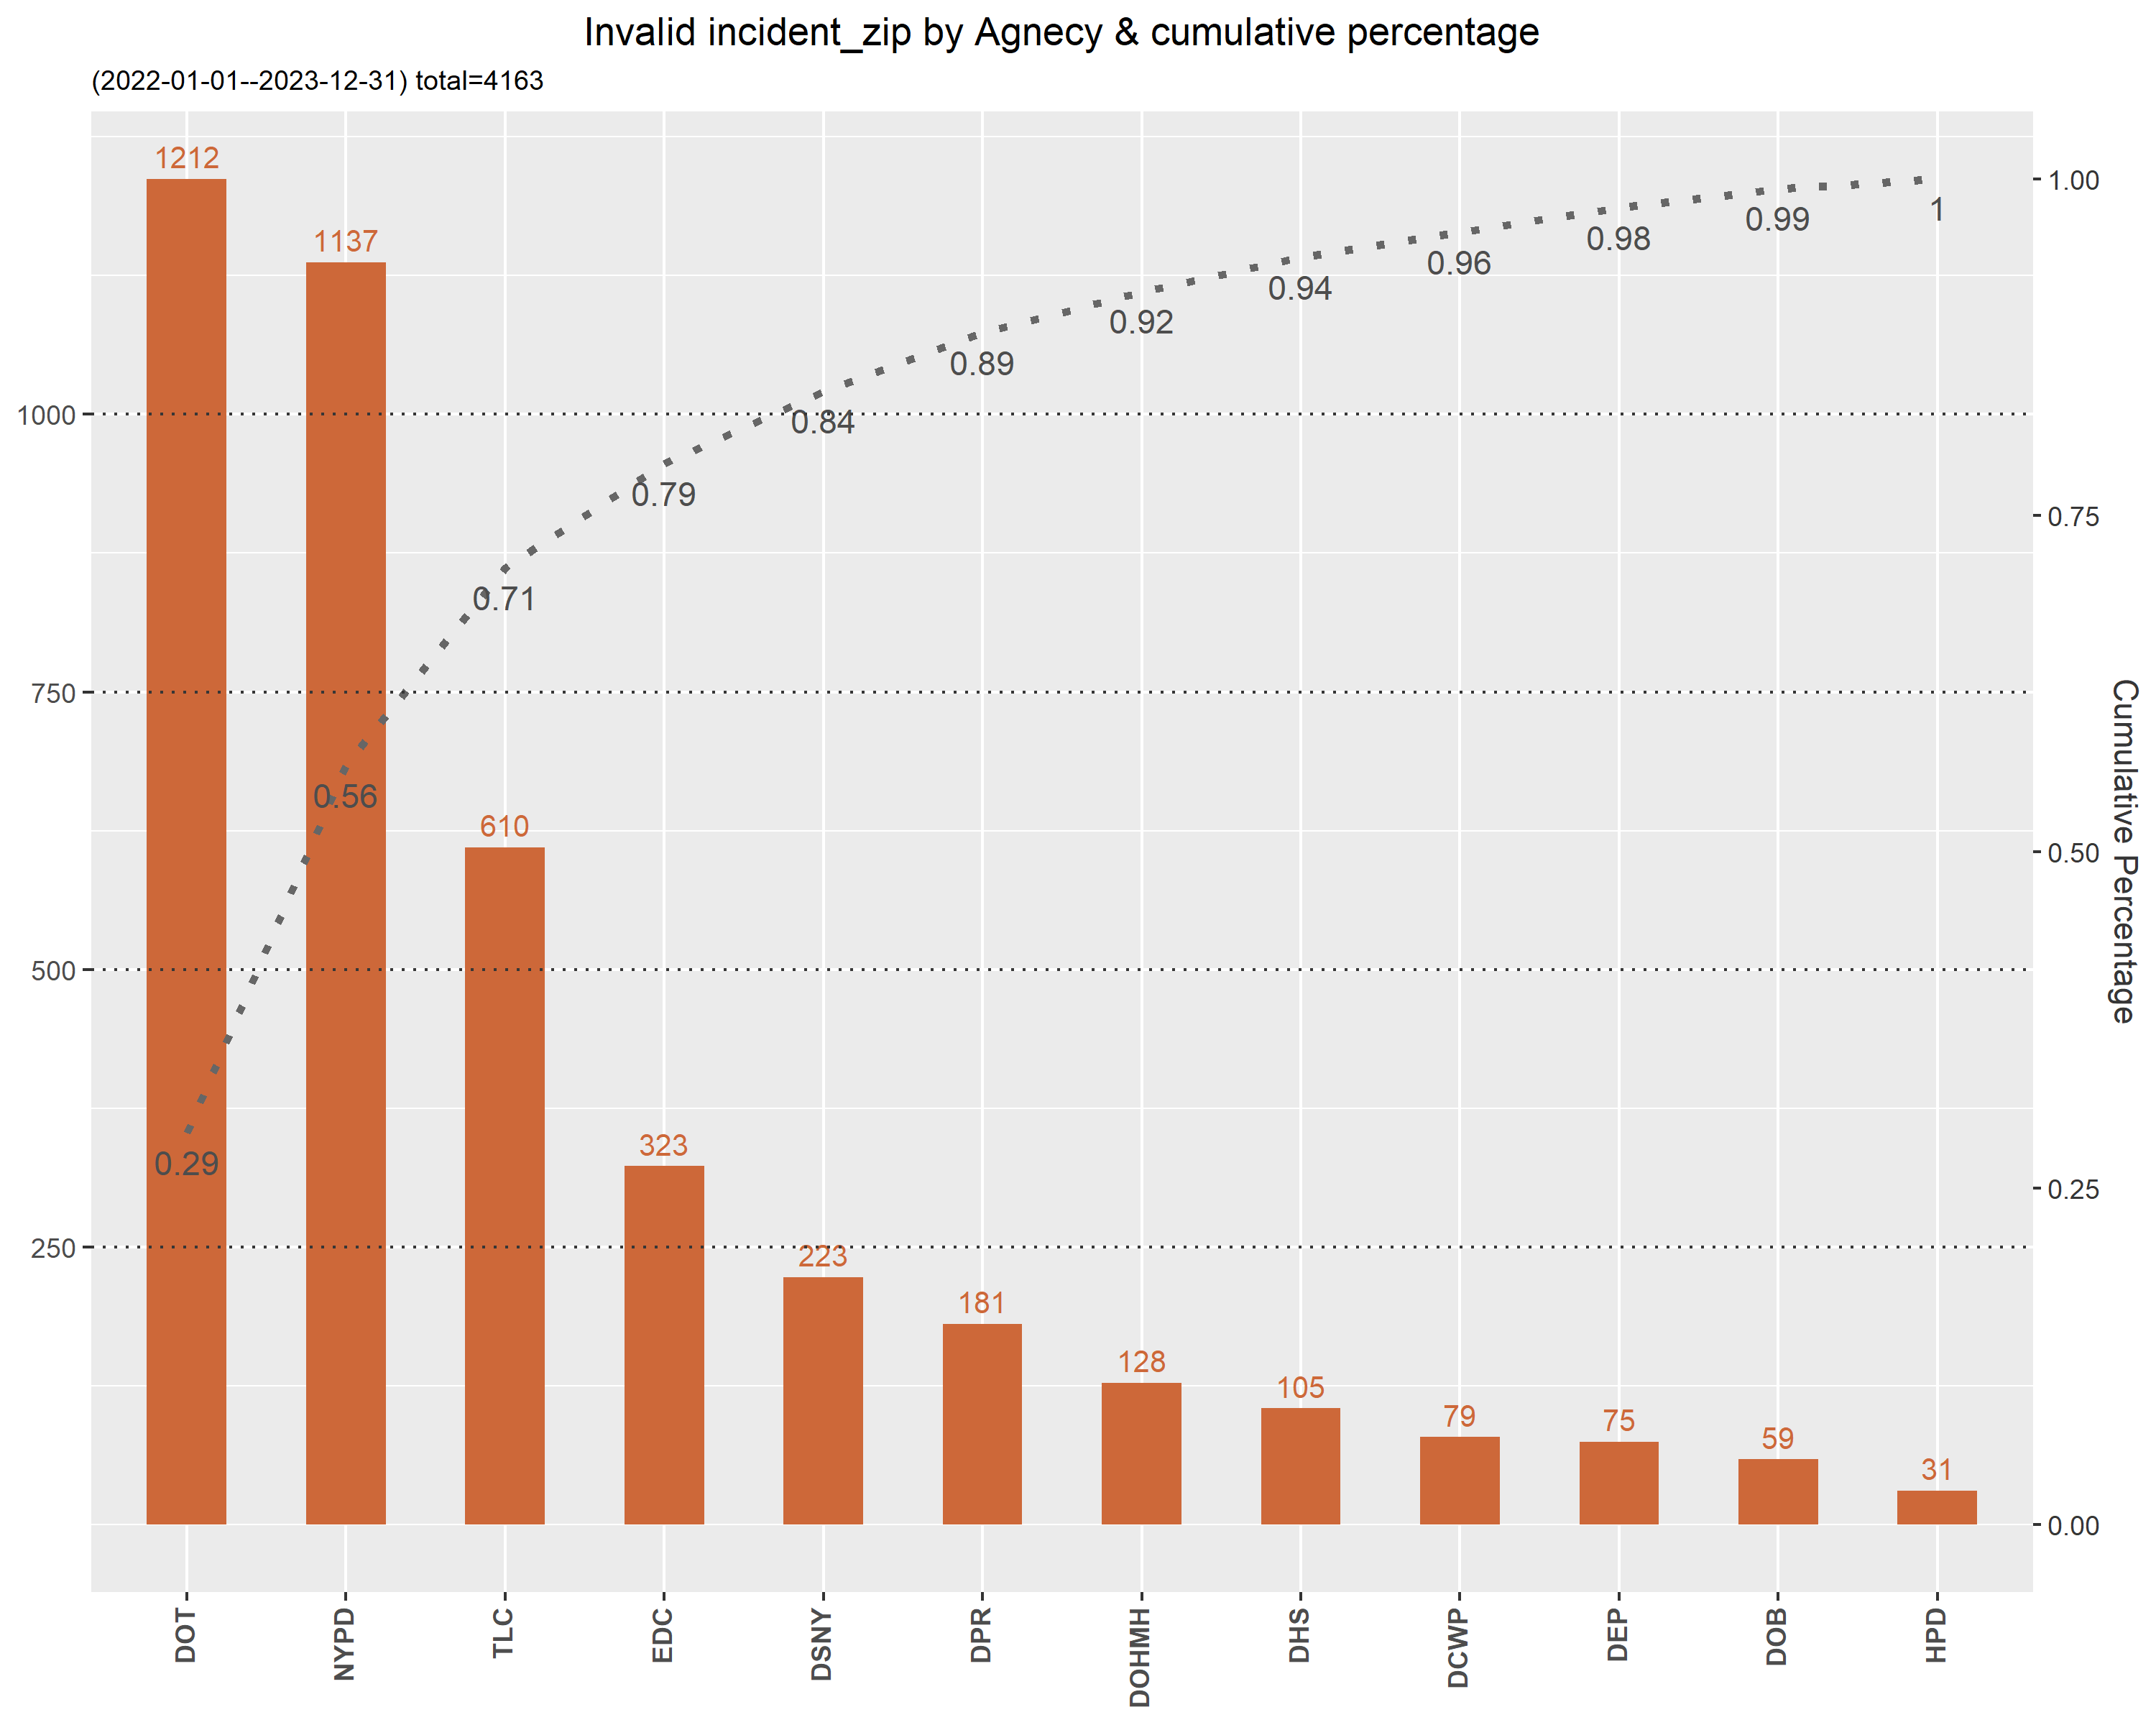
\includegraphics[width=\textwidth]{invalid_incident_zip.png}
		  \caption{Invalid incident-zip by Agency}
		  \label{fig:invalid_incident_zip}
	\end{figure}
	
		\subsubsection{Case Study: Noise Complaints by Zip Code}
		\textbf{Scenario:} The NYC Office of Nightlife (ONL) wants to know ``What are the top 10 zip codes for Noise Complaints (all 8 types) over the last two years?''
		The goal is to assess the impact of the recent NYC effort looking to promote a safe and vibrant nightlife scene in NYC while seeking to ease
		strained relations between bar and club owners. 
		
		It may come as a surprise to non-NYC residents that dancing at bars and restaurants has been illegal since 1926 (during prohibition), and was only just repealed in 2018. 
		
		On the surface this would seem like a simple effort.  The NYC Open Data Portal allows for selection of a timeframe (2022-2023), complaint-type
		begins with ``Noise'', and group by Zip code, sorted descending by count.  You can do this analysis and grouping right inside the NYC Open Data Portal. \textit{Voila!}

	\begin{figure}[H]
	    		\centering
	    		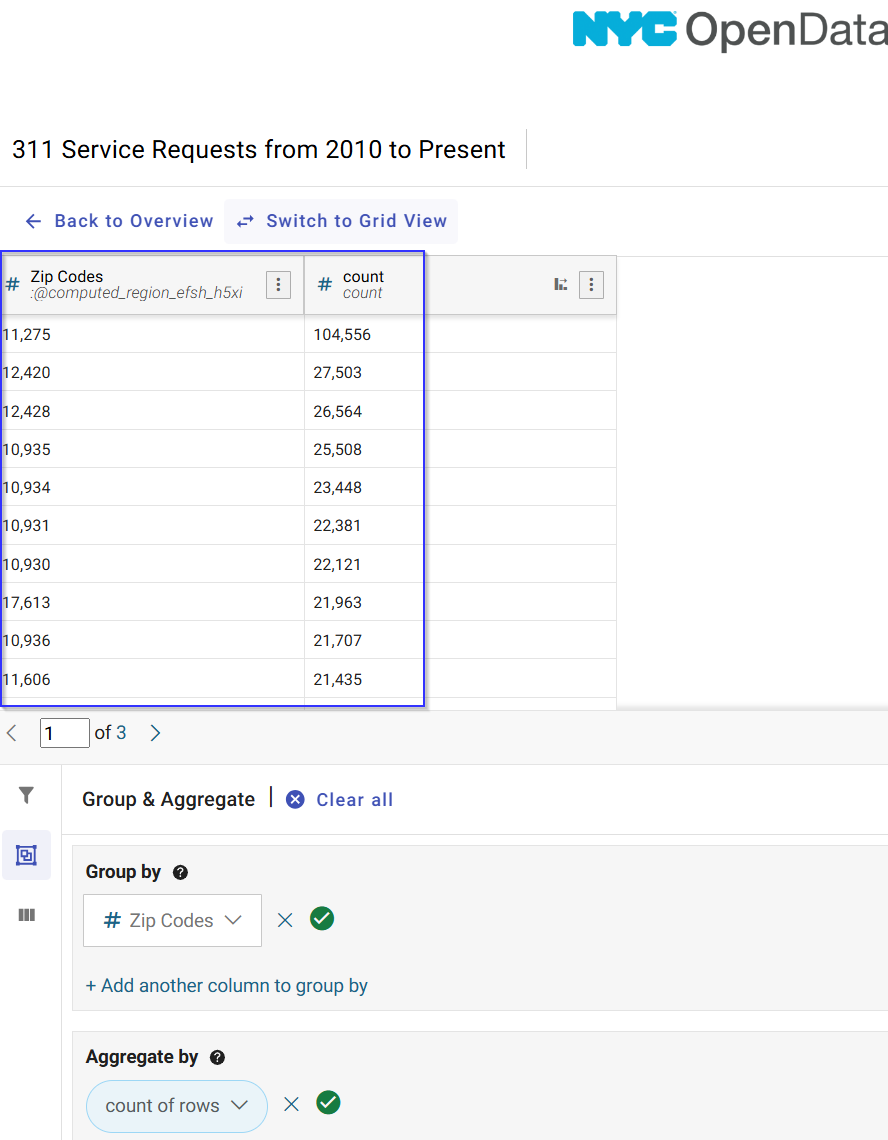
\includegraphics[scale = 0.6]{zipcode_casestudy.png}
	    		\caption{Top 10 zip codes for Noise complaints (Zip Codes)}
	    	\label{fig:casestudy1-zipcodes}
		\end{figure}
	
		However, this analysis uses the zip\_codes field, one of the (six) computed fields that has shown to have validity problems. If we repeat the analysis with the 
		incident\_zip field instead of the zip\_codes field, we obtain a different set of zip code results:
		
		\begin{figure}[H]
	    		\centering
	    		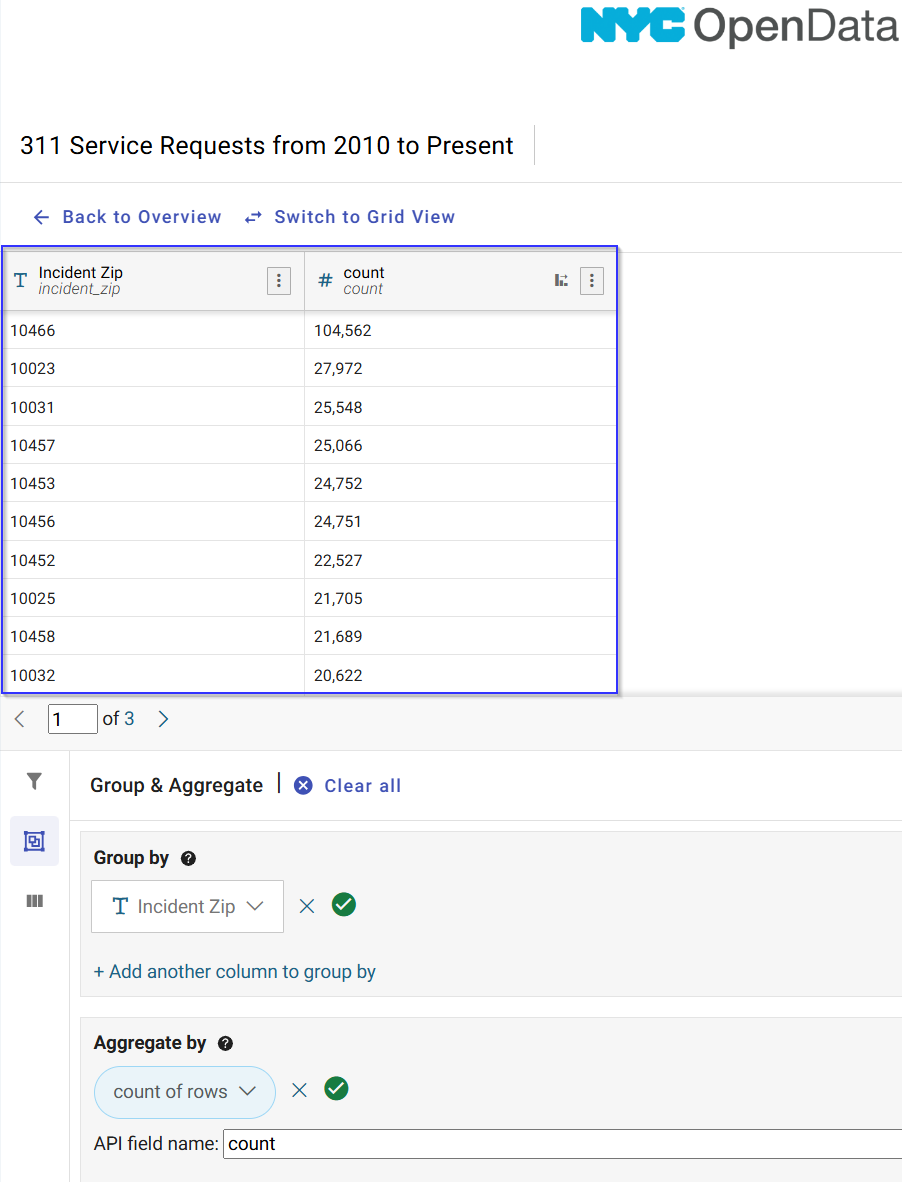
\includegraphics[scale = 0.6]{incident_zip_casestudy.png}
	    		\caption{Top 10 zip codes for Noise complaints(Incident Zip)}
	    	\label{fig:casestudy1-incident-zip}
		\end{figure}
		
	Let's subject these two data sets to validation against the US Postal Service zip code database.
	 
	\begin{table}[H]
	\centering
	\footnotesize
	\begin{tabular}{lrr@{\hskip 0.5cm}|@{\hskip 0.5cm}lrr}
	\toprule
	\multicolumn{3}{c}{\textbf{zip\_codes}} & \multicolumn{3}{c}{\textbf{incident\_zip}} \\
	\cmidrule(r){1-3} \cmidrule(l){4-6}
	\textbf{Zip Code} & \textbf{Count} & \textbf{Valid?} & \textbf{Zip Code} & \textbf{Count} & \textbf{Valid?} \\
		\midrule
		11275 & 104,556 & FALSE & 10466 & 104,562 & TRUE \\
		12420 & 27,503 & TRUE & 10023 & 27,972 & TRUE \\
		12428 & 26,564 & TRUE & 10031 & 25,548 & TRUE \\
		10935 & 25,508 & FALSE & 10457 & 25,066 & TRUE \\
		10934 & 23,448 & FALSE & 10453 & 24,752 & TRUE \\
		10931 & 22,381 & TRUE & 10456 & 24,751 & TRUE \\
		10930 & 22,121 & TRUE & 10452 & 22,527 & TRUE \\
		17613 & 21,963 & FALSE & 10025 & 21,705 & TRUE \\
		10936 & 21,707 & FALSE & 10458 & 21,689 & TRUE \\
		11606 & 21,435 & FALSE & 10032 & 20,622 & TRUE \\
		\bottomrule
	\end{tabular}
	\caption{Comparison of Top Ten Zip Codes Lists}
	\end{table}

	As indicated, six out of ten zip\_codes are invalid, which corresponds closely with what is observed in the overall dataset (58\%). Whereas the incident\_zip
	field is completely valid, again in-line with the overall incident\_zip validation percentage (99.04\%). If the analysis performed using the zip\_codes field were to be
	presented to the Drirectror, ONL, the conclusion would be in error. Perhaps more curious than the differing zip codes on the two lists, 
	is the fact that the numerical counts are nearly identical;  the overall counts are quite close. This is curious since
	one field is computed while the other is via data entry; the computed protocol is again the suspect. The algorithm appears to be counting corrrectly (or nearly so)
	but mis-identifying the corresponding zip code.

	
	\subsection{Issues with Police Precincts}
	A curious case also exists when examining the two nearly identical fields - police\_precincts and police\_precinct. Both of those fields are among
	the ``computed'' fields in the dataset. 
	Using \href{https://www.nyc.gov/site/nypd/bureaus/patrol/precincts-landing.page}{NYPD Precinct listings} it's possible to determine the valid
	police precincts; they are generally numeric or have numeric representations in the dataset. 
	
	However, what we find is that both fields police\_precinct and police\_precincts  have  35\% invalid entries.
	Unfortunately, they're not the same invalid entries. 
	
	For the police\_precincts field, there are 2,171,864 invalid entries (35\%)., a consequential number of errors. Similarly for the police\_precinct field,
	 there are 2,171,778 invalid entries ( also 35\%), however they are not the same counts for the two similar fields.

	The top ten (by count) of invalid precincts for each field are:

	\begin{table}[ht]
	\footnotesize
	\centering
		\begin{tabular}{ccccc}
		\toprule
		\textbf{Invalid Precinct} & \textbf{police\_precinct count} & \textbf{police\_precincts count} & \textbf{Delta}\\
		\midrule
			62 & 151808 & 151720 & 88 \\
			72 & 148881 & 148796 & 85 \\
			67 & 133171 & 133115 & 56 \\
			64 & 111236 & 111221 & 15 \\
			60 & 105252 & 105317 & -65 \\
			65 & 103334 & 103306 & 28 \\
			53 & 100097 & 100074 & 23 \\
			73 & 97746 & 97755 & -9 \\
			68 & 94204 & 94254 & -50 \\
			66 & 93654 & 93848 & -194 \\
		\bottomrule
		\end{tabular}
	\caption{Comparison of the fields police\_precinct and police\_precincts}
	\label{tab:comparison-precincts-diff}
	\end{table}
	
	A graphic representation of the invalid police\_precincts plotted by Agency show a near perfect match to the
	distribution of the entire 6.4 million SRs as seen in Figure \ref{fig:SR_counts_by_Agency}. Note that the ``big six'' Agencies account for 90\% of these invalid precinct errors, identical
	to the overall distribution of all SRs. (The same is true for a similar graph of by the police\_precint field.) This strongly suggests that this is a systemic problem, almost certainly caused by the computation method applied for these two fields.
	 
	\begin{figure}[H]
	  \centering
		  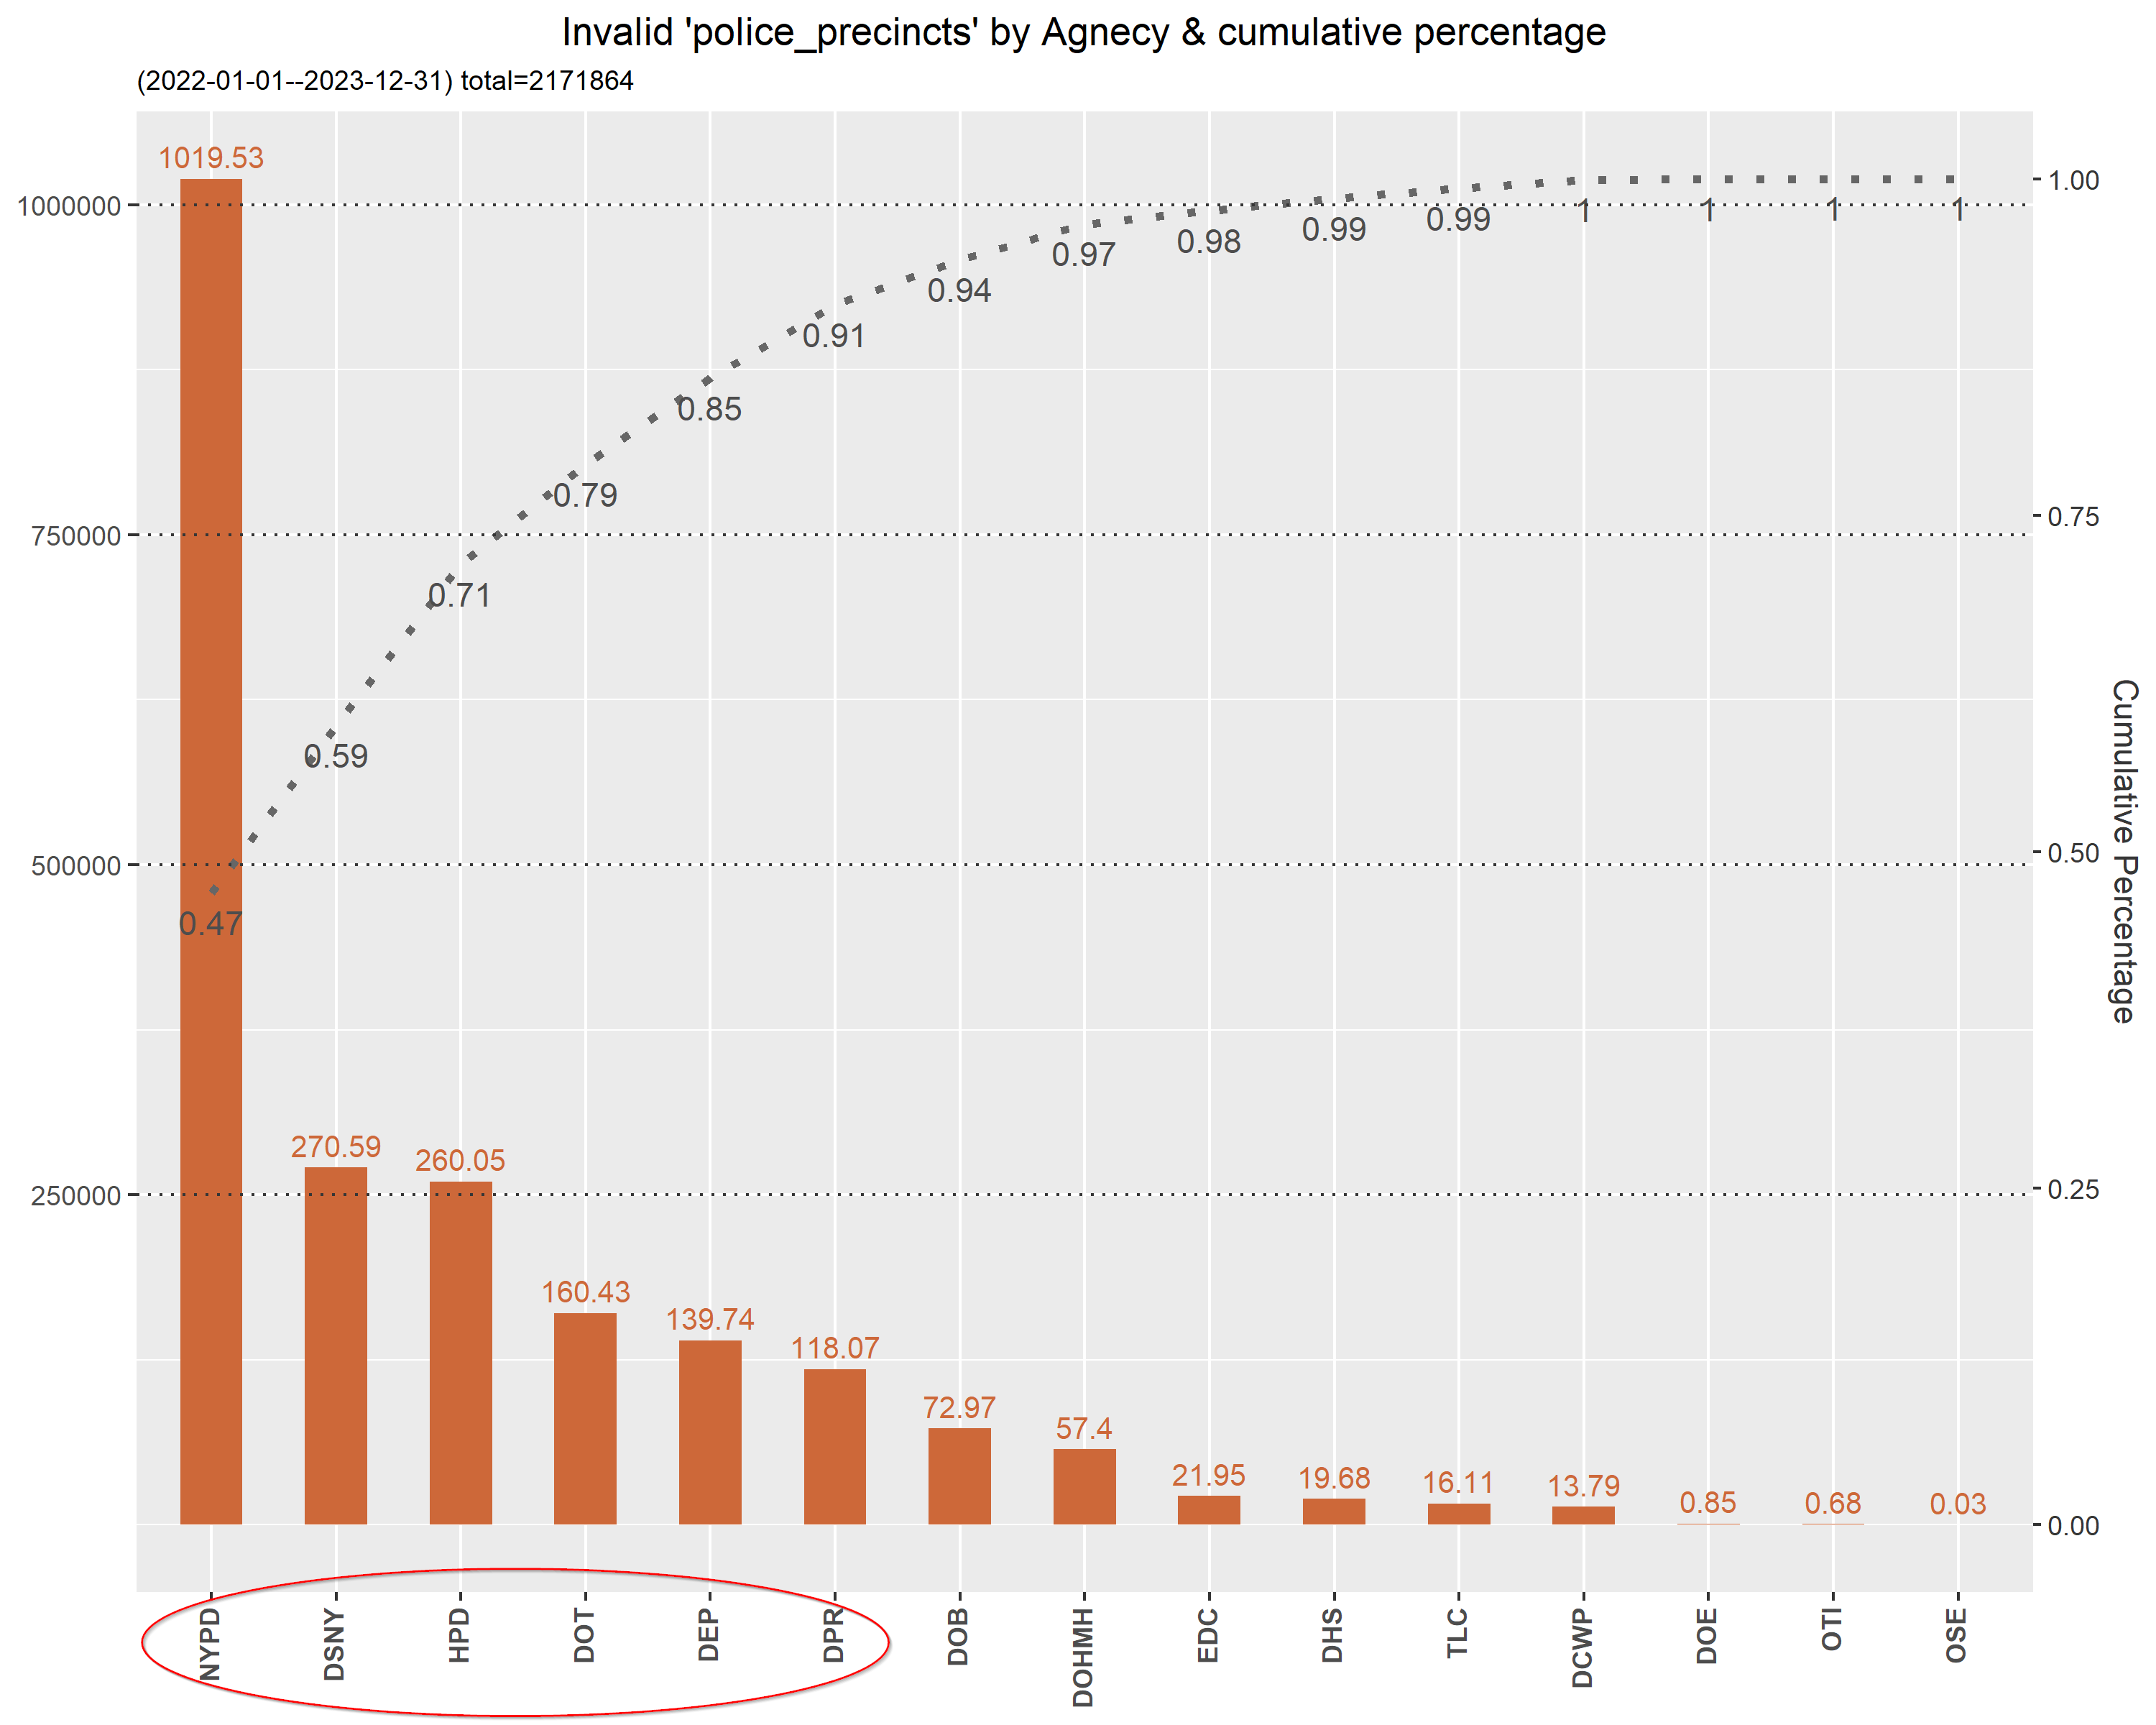
\includegraphics[width=\textwidth]{invalid_police_precincts.png}
		  \caption{Invalid NYPD precincts by Agency}
		  \label{fig:invalid_police_precincts_zip}
	\end{figure}

	\subsection{Issues with Community Boards}
	Community Boards are an important aspect of NYC government. They are the most local, grassroots form of City government, 
	and a vital connection between communities and elected officials and City agencies. They are organized by the five Boroughs of NYC and represented
	in this dataset as ``\#\#-Borough'', e.g. ``10 Bronx'' and report to the various Borough Presidents in NYC. As such, they play an important role in the quality of life for all New Yorkers.
	There are 59 community boards throughout the City: 12 Community Districts in the Bronx, 18 in Brooklyn, 12 in Manhattan, 14 in Queens and 3 in Staten Island.
	The Community Boards are used frequently as a way to measure distribution of City services throughout the five boroughs, so correctness is important. 
	NYC Borough Presidents in particular are focused on the services offered at the Community Board level within their respective Borough.
	
	In the 2022-2023 dataset there are 27,276 invalid community\_board entries which represents 0.43\% of non-blank data. 
	There are a total of 12 different invalid community boards, to include: 
	
		\begin{table}[H]
		\centering
		\footnotesize
		\begin{tabular}{rlr}
		\toprule
		\textbf{Rank} & \textbf{Invalid CB} & \textbf{Count} \\
			\midrule
				1 & 64 MANHATTAN & 7144 \\
				2 & 83 QUEENS & 5133 \\
				3 & 55 BROOKLYN & 3327 \\
				4 & 81 QUEENS & 3180 \\
				5 & 80 QUEENS & 2407 \\
				6 & 26 BRONX & 2364 \\
				7 & 28 BRONX & 1128 \\
				8 & 82 QUEENS & 1054 \\
				9 & 95 STATEN ISLAND & 515 \\
				10 & 27 BRONX & 514 \\
			\bottomrule
		\end{tabular}
		\caption{Top Ten Invalid 'community\_board' Values}
		\end{table}
		
		The distribution of invalid Community Boards by Agency is not consistent with the overall SR Agency distribution. This indicates that there are likely
		specific issues at some key Agencies, in this case Taxi \& Limo Commission (TLC), Parks \& Recreation, etc. It's not a large error, but the division of services
		(and complaints) by Community Board is a well-tracked measure so accuracy is again important.

		\begin{figure}[H]
	 	 \centering
		  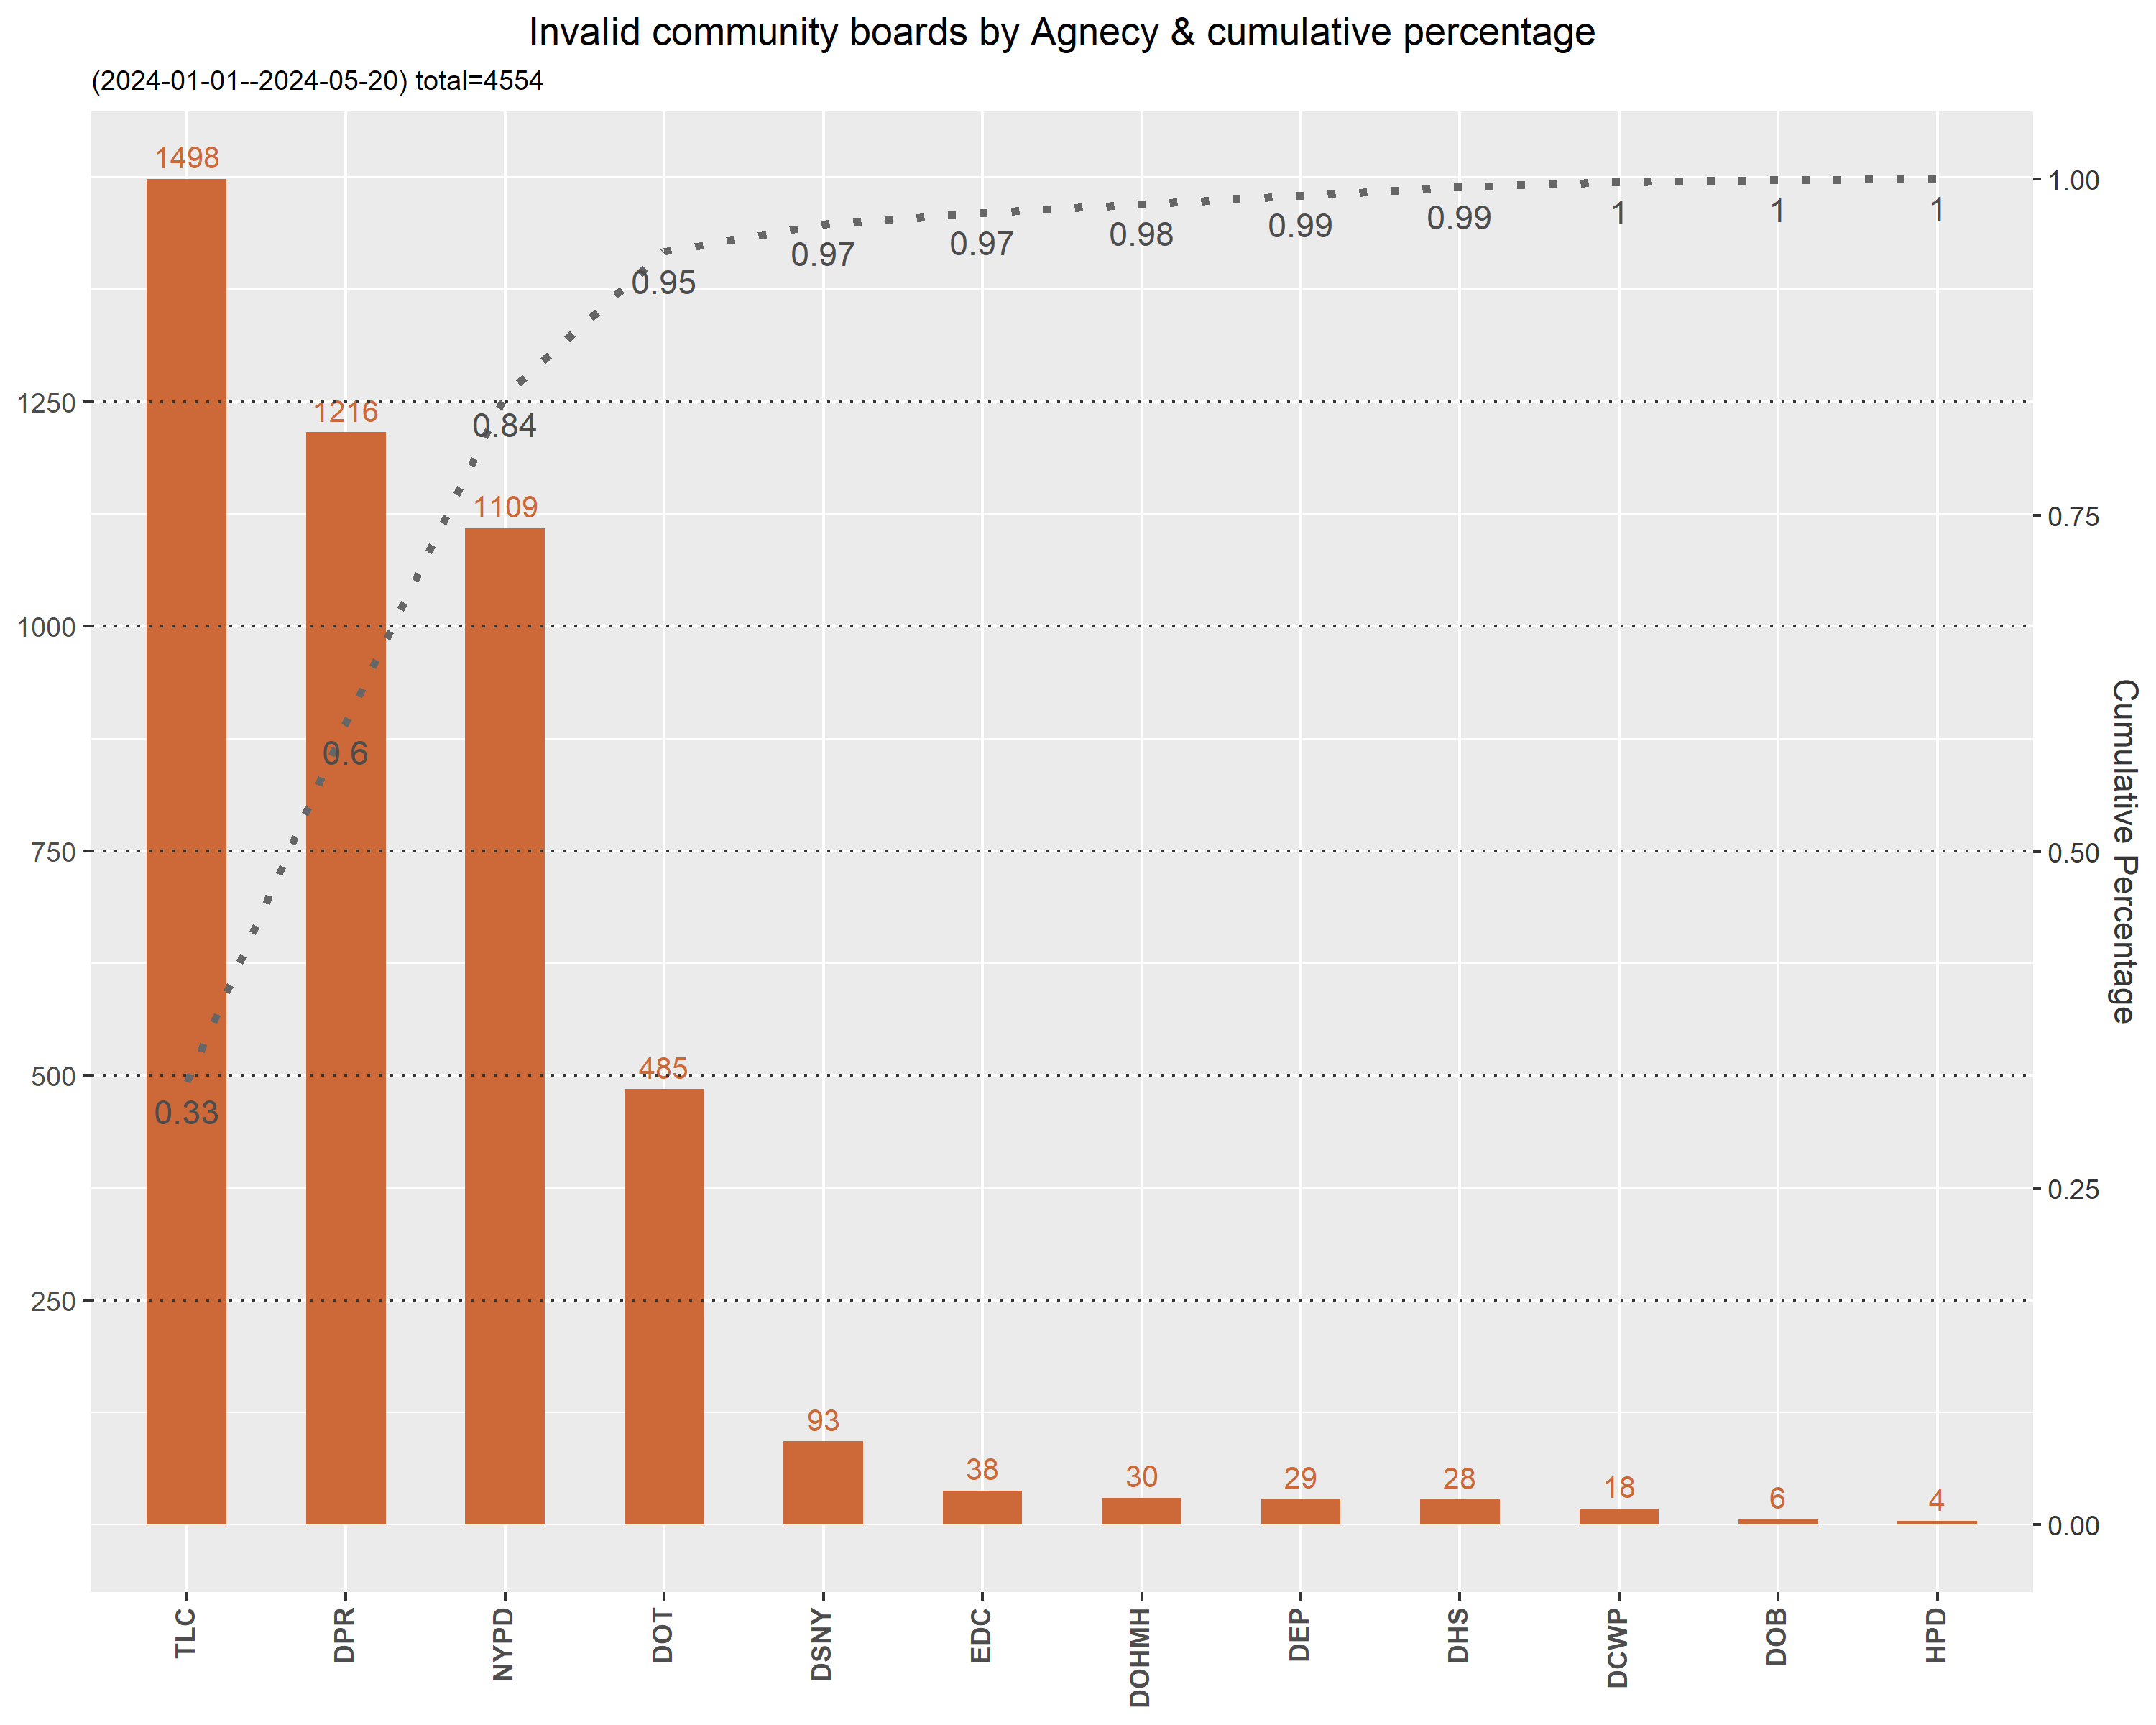
\includegraphics[scale = 0.65]{invalid_community_boards.png}
		  \caption{Invalid Community Board by Agency}
		  \label{fig:invalid_community_boards}
		\end{figure}


	\subsection{Issues with Community Districts}
	Another of the computed fields is community\_districts. Community Districts are the boundaries for the Community Boards, but unlike how Community Boards are
	an arm of the government of New York City, the Community District is used by the Department of City Planning (DCP) for purposes of environmental, socio-economic, and
	demographic purposes. DCP is the NYC''s primary land use agency and is instrumental in the City's physical framework.  It is a geographical division rather
	than a local government division. And like Community Boards, the Community Districts are frequently cited as a means to track zoning, housing, community facilities,
	and waterfront/open/public spaces. It is another of the NYC well-tracked measures.

	Due to how the community\_district data is formatted, it is not possible to establish validity. However, it is possible to determine that the dataset contains
	72 unique entries, while there are only 59 valid Community Districts. So it would appear that there are 13 invalid commuity\_board(s) contained in the dataset.
	
	
	
\section{Inconsistent \& Unusual Patterns with Dates}\label{sec:inconsistencies}

As previously mentioned, the dataset has four data fields:  created\_date, closed\_date, due\_date, and resolution\_action\_update\_date.
The due\_date field has few entries to analyze; 99.62\% of due\_date entries are ``N/A''.  It is not known if the due\_date(s) are truely
``not applicable'' or that the due\_date field is rarely used. The  resolution\_action\_update\_date field serves as a date-time marker
showing when the SR record was last updated.  All the date fields are recorded to the second, e/g/ ``2022-02-11 13:43:05''.

\subsection{created\_date and closed\_date(s) -- Negative Duration}
Let's look first at the created\_date and closed\_date fields. You might expect that these two fields are automatically populated by the 
SR application software, either the software used at the 311 organization or that used at the Agencies that are integrated with the 311 system;
and typically that is indeed the case. In such a case, the act of creating an SR would automatically trigger an entry in created\_date based on a system-wide clock. Thus
the created\_date is associated with setting an SR status to ``new'' or ``open''. And similarly when an SR's status is changed to
``closed'' then the closed\_date would be populated. 

Unfortunately, our analysis found that that assumption is not always the case. When you analyze the various date fields, several
anomalies become quickly apparent:

	\begin{itemize}
		    \item Some SRs have a closed\_date that occurs before the created\_date.
		    \item Some created\_date(s) and closed\_date(s) appear either in the future or in the far distant past.
		    \item There are a large number of SRs that are closed and created exactly at midnight or exactly at noon. 
	\end{itemize}

\textbf{Why are these date fields important?} They're important because citizens, NYC Government Officials, and NYC Agencies use these dates
to measure the responsiveness for providing the services. How long does it take to replace an out-of-order street light?
How rapid is the response to a report of domestic violence? Does the NYPD response to a noise complaint in Staten Island take
longer than in Manhattan? How long does it take to repair a street pothole in Queens? 

The measure of ``duration'', of the response time of a 311 call is a closely watched, carefully scrutinized metric, 
both in terms of overall performance and with a geographical area. And it can have broad political, organizational,
and budgetary consequences. Duration is not a field in the dataset, but it is easily computed by closed\_date - created\_date.
Let's look at some anomalies in this ``duration'' field.

Closed-before-Created:  There are 12,251 SRs that are closed before they were created, thereby generating a nonsensical 
``negative duration''. While this is a small percentage overall (0.2\%) it can have significant impact on response time analysis.
In most cases, these ``negative durations'' appear to just be mistakes. Here is a sample of some of the largest and the
smallest errors:

\begin{table}[H]
    \centering
    \small
    \begin{tabular}{>{\ttfamily}l l l r l}
        \toprule
        \multicolumn{5}{c}{\textbf{Largest errors (days) excluding extreme negative values}} \\
        \midrule
        \textbf{created\_date} & \textbf{closed\_date} & \textbf{duration} & \textbf{agency} \\
	        \midrule
	        2023-01-27 14:40:00 & 2022-01-14 14:40:00 & -378.000000 & DOT \\
	        2023-01-18 10:06:00 & 2022-01-12 10:06:00 & -371.000000 & DOT \\
	        2023-01-27 14:36:00 & 2022-01-22 14:35:00 & -370.000694 & DOT \\
	        2023-01-11 11:10:00 & 2022-01-09 11:10:00 & -367.000000 & DOT \\
	        2023-12-18 03:13:00 & 2023-01-16 13:10:00 & -335.585417 & DOT \\
	        \midrule
	        \multicolumn{5}{c}{\textbf{Smallest errors (days)}} \\
	        \midrule
	        \textbf{created\_date} & \textbf{closed\_date} & \textbf{duration} & \textbf{agency} \\
	        \midrule
	        2023-06-28 07:07:31 & 2023-06-28 07:07:00 & -0.000359 & DOT \\
	        2023-06-29 09:10:20 & 2023-06-29 09:10:00 & -0.000231 & DOT \\
	        2023-01-12 06:50:13 & 2023-01-12 06:50:00 & -0.000150 & DOT \\
	        2023-06-26 08:09:07 & 2023-06-26 08:09:00 & -0.000081 & DOT \\
	        2023-01-12 06:51:01 & 2023-01-12 06:51:00 & -0.000012 & DOT \\
	        \bottomrule
    \end{tabular}
    \caption{Largest and Smallest errors (days)}
    \label{tab:combined_errors}
\end{table}

The largest errors are shown ``excluding extreme negative values''. We found eight SRs with extremely large negative durations (< -730),
all containing an entry of ``1900-01-01'' as the closed\_date, which generates extremely large negative durations exceeding 44,601 days (122 yrs).
That large of an anomaly can skew statistical results, even though the number of occurrences is small. This is especially curious
as the date ``1900-01-01'' is also the earliest date that Microsoft Excel can accommodate as well as how Excel treats a blank
cell that is designated as a date. All raising suspicions that perhaps these dates were imported into the 311 system from Excel.

According, these  SR rows are removed from the box \& whiskers plot. Note that these extremely large negative duration SRs all
are from the Department of Homeland Services (DHS) Sample: 

\begin{table}[H]
    \centering
    \small
    \begin{tabular}{l l r l}
        \toprule
        \textbf{created\_date} & \textbf{closed\_date} & \textbf{duration} & \textbf{agency} \\
	        \midrule
	        2022-02-11 13:43:05 & 1900-01-01 & -44601.571586 & DHS \\
	        2022-02-11 11:03:38 & 1900-01-01 & -44601.460856 & DHS \\
	        2022-02-11 08:29:49 & 1900-01-01 & -44601.354039 & DHS \\
	        2022-02-11 14:08:08 & 1900-01-01 & -44601.588981 & DHS \\
	        2022-02-11 14:05:16 & 1900-01-01 & -44601.586991 & DHS \\
	        \bottomrule
    \end{tabular}
    \caption{Sample of SRs with extremely large negative durations}
    \label{tab:extreme_negative_durations}
\end{table}

Here is a graphic visualization of the negative-duration SRs by Agency. It is obvious that this
negative-duration issue is a problem at the Dept. of Transportation (DOT) where 95\% of these
types of errors occur. 

\begin{figure}[H]
 	 \centering
	  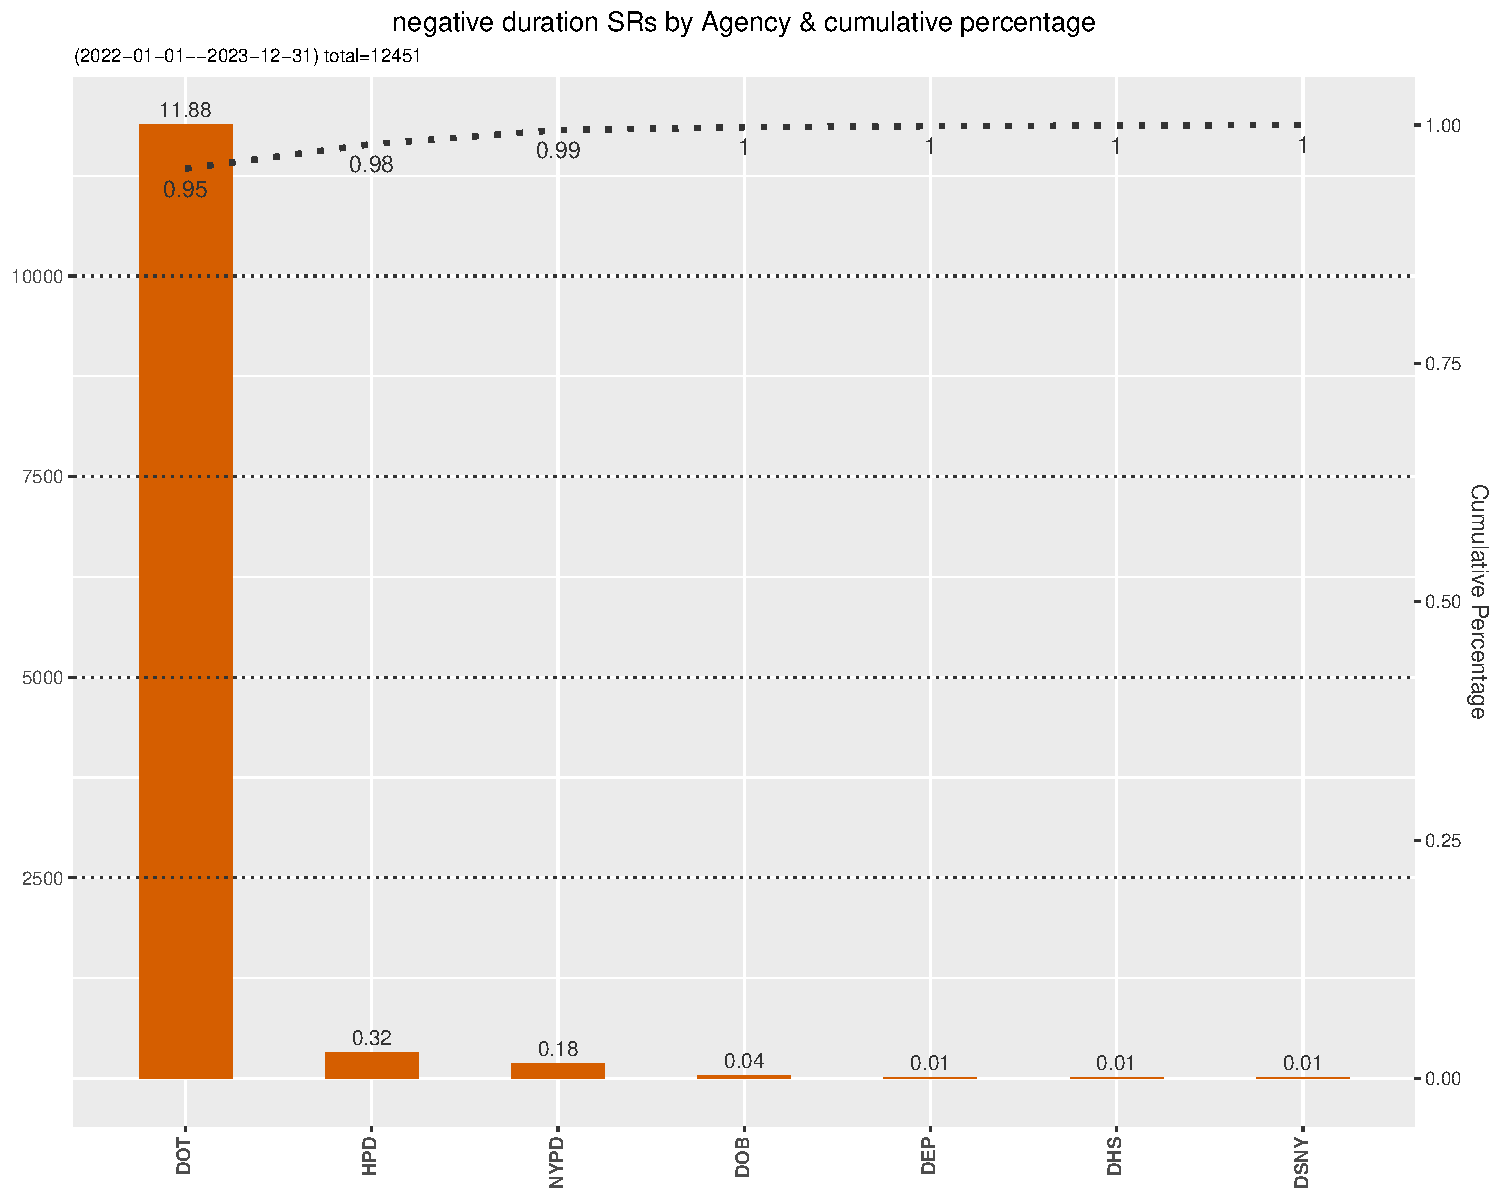
\includegraphics[scale = 0.65]{negative_duration_SR_barchart.png}
	  \caption{SRs with a Negative Duration by Agency}
	  \label{fig:negative-duration}
\end{figure}

This violin chart shows the broad spread of negative-duration SRs, albeit with the extremely large 
negative-duration SR removed. While there are few outlier points, the magnitude of the negative-durations
is troubling and can produce bizarre analytical results.

\begin{figure}[H]
 	 \centering
	  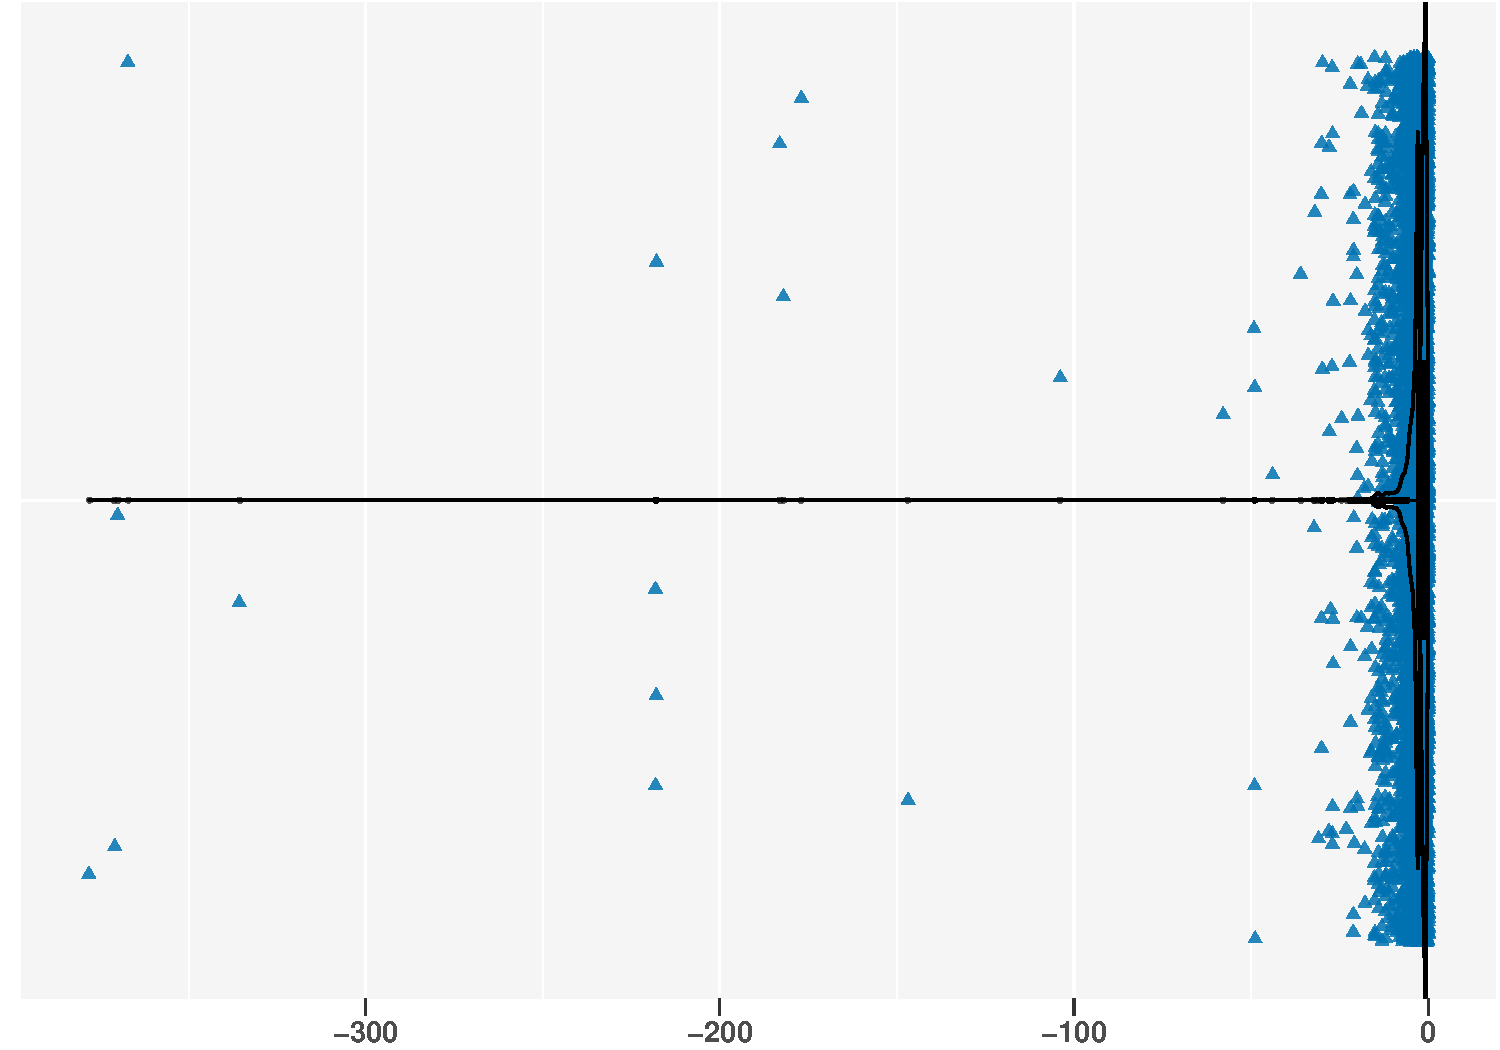
\includegraphics[scale = 0.65]{negative_duration_SR_violin.png}
	  \caption{Negative duration distribution}
	  \label{fig:negative-duration-violin}
\end{figure}


\subsubsection{Case Study: Homeless Person Assistance}
		\textbf{Scenario:} The Dept. of Homeless Services wants to know ``How quickly are 311 calls for ``Homeless Person
		Assistance over the past two years?'' resolved. This is a typical request made by both the public and City government. It's a performance metric along the lines
		of ``How quickly is my Agency responding to ``critical'' requests, and does that performance vary by Borough, Zip Code, etc. 

		As an analyst, this appears to be a routine effort: 
		
		\begin{enumerate}
		    \item Select data from 2022-2023 and filter the data by complaint\_type = ``Homeless Person Assistance'' (yields 55,000 SRs)
		    \item Compute a new field ``duration'' (closed\_date – created\_date)
		    \item Take an average of the ``duration'' field == \textbf{Answer:  -4.8 days}  
		\end{enumerate}
		
		Clearly that answer is nonsensical. How did such a simple task result in an absurd answer? The answer lies in the computation of the
		``duration'' field. As it turns out, there are eight DHS SRs that have a closed\_date of ``1900-01-01''. Each of those SRs creates a 
		negative duration of -44,602 days (-122 years). So just those eight SRs with extreme negative duration values is enough to drive
		the average of the 75,000 Homeless Assistance SRs to a negative value, clearly incorrect.
		
		As it turns out the distribution of the ``Homeless Person Assistance'' is quite skewed due to a small number of long duration
		SRs. In this case, the median is a better measure of central tendency than the average. And the median of the duration
		field is  0.2 days (approx 5 hrs). Here is a look at the distribution of durations for the Homeless Person Assistance SRs showing
		the large outliers. 
		
		\begin{figure}[H]
		 	 \centering
			  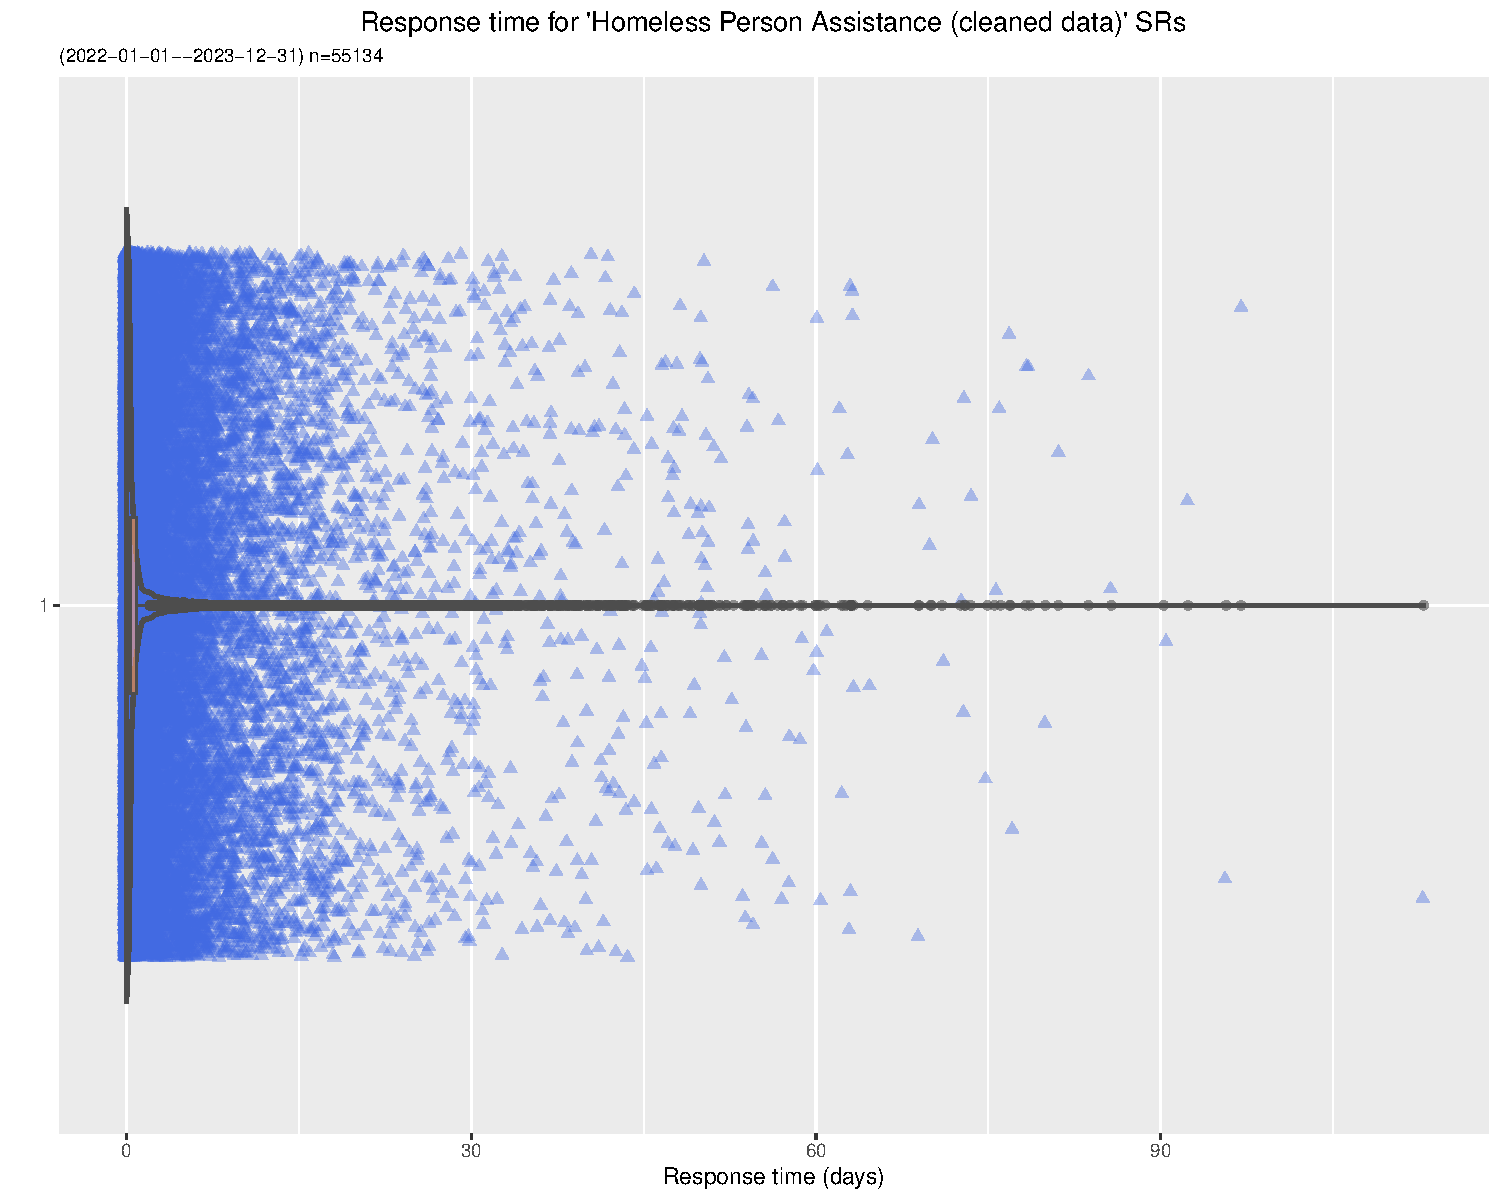
\includegraphics[scale = 0.65]{homeless_response_time_clean.png}
			  \caption{Homeless Assistance SR Durations}
			  \label{fig:homeless}
		\end{figure}
		
	\subsection{created\_date and closed\_date(s) --  Zero Duration}		
	An even more serious, and more prevalent problem with closed\_date(s) occurs when the closed\_date and created\_date
	are exactly the same -- to the second -- which accordingly creates a \textbf{zero duration'}. Again this is nonsensical, but the
	presence of such zero durations can again severely distort analytics. There are 191,141 such SRs representing 3.1\% of all 
	non-blank data; not an insignificant number. As shown in the chart below, 99\% of the zero duration SRs appear to predominately
	occur in five Agencies (Dept of Mental Health \&Hygine, Dept of Transportation, Dept of Business, Dept of Sanitation,
	and Dept of Environmental Protection.) This is not in-line with the overall Agency distribution of SRs and indicates an
	Agency-specific issue, and the solution likely lies at those Agencies.
	
	\begin{figure}[H]
		 \centering
		 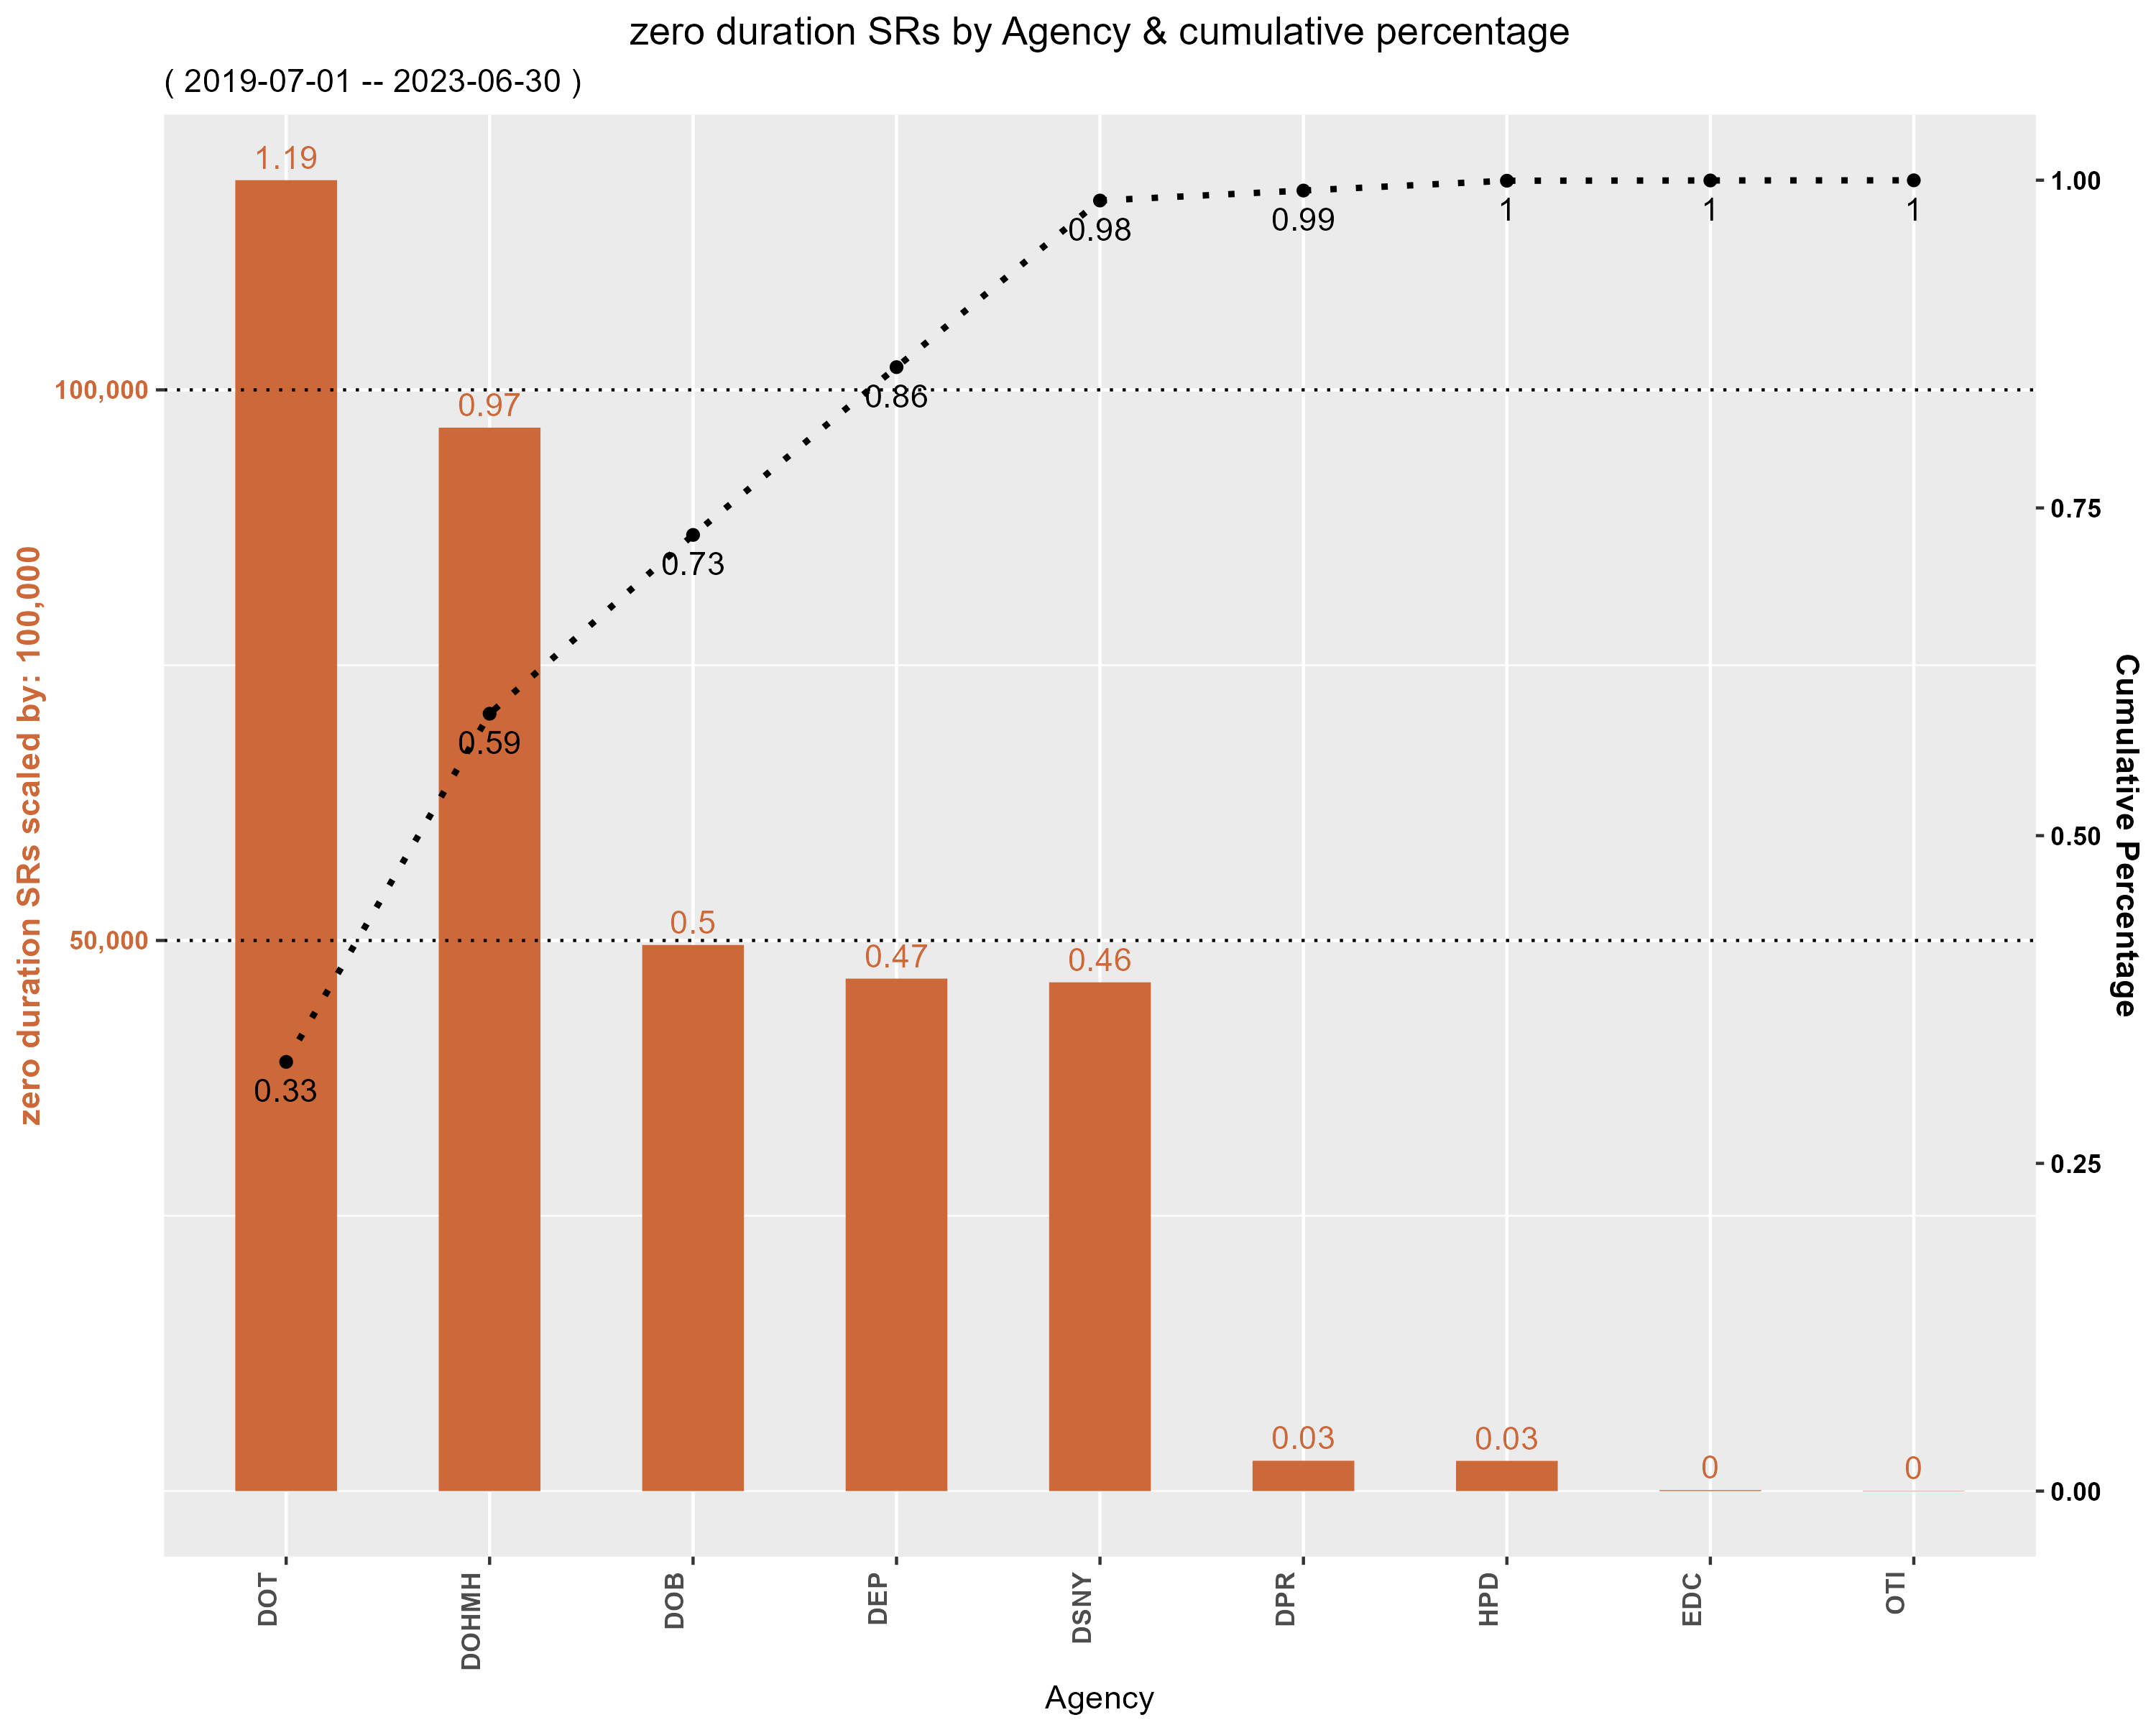
\includegraphics[scale = 0.65]{zero_duration_SR.png}
		 \caption{SRs with Zero Durations by Agency}
		 \label{fig:sero-duration}
	\end{figure}	
		
	\subsection{created\_date and closed\_date(s) -- Midnight \&Noon}
	One final problem discovered with the created\_date and closed\_date; there appears to be an unusual number of exactly
	midnight and noon date-time values for these two fields. The distribution of SR creation largely follows the clock; lots of
	SRs created during day-light hours and much fewer created in the early hours of the morning. However, there appears
	to be significantly greater numbers of SR both created and closed exactly at midnight, and exactly at noon. The reason this
	issue is worth investigating, goes back to the ``duration'' question -- if SRs are used as a source to measure responsiveness
	for the delivery of services, and if those times are not an accurate reflection of the start/finish of the Service, then the
	duration is in question. Observations during this 2-year period:
	
	\begin{itemize}
		    \item  there are 7210 SRs created exactly at midnight
		    \item There are 99,779 SRs created exactly at noon.
		    \item There are 105,505 SRs closed exactly at noon. 
		    \item There are 235,347 SRs closed exactly at midnight
	\end{itemize}
	
	Let's look SRs are created and closed by the hour of the day :
	
	\begin{figure}[H]
		 \centering
		 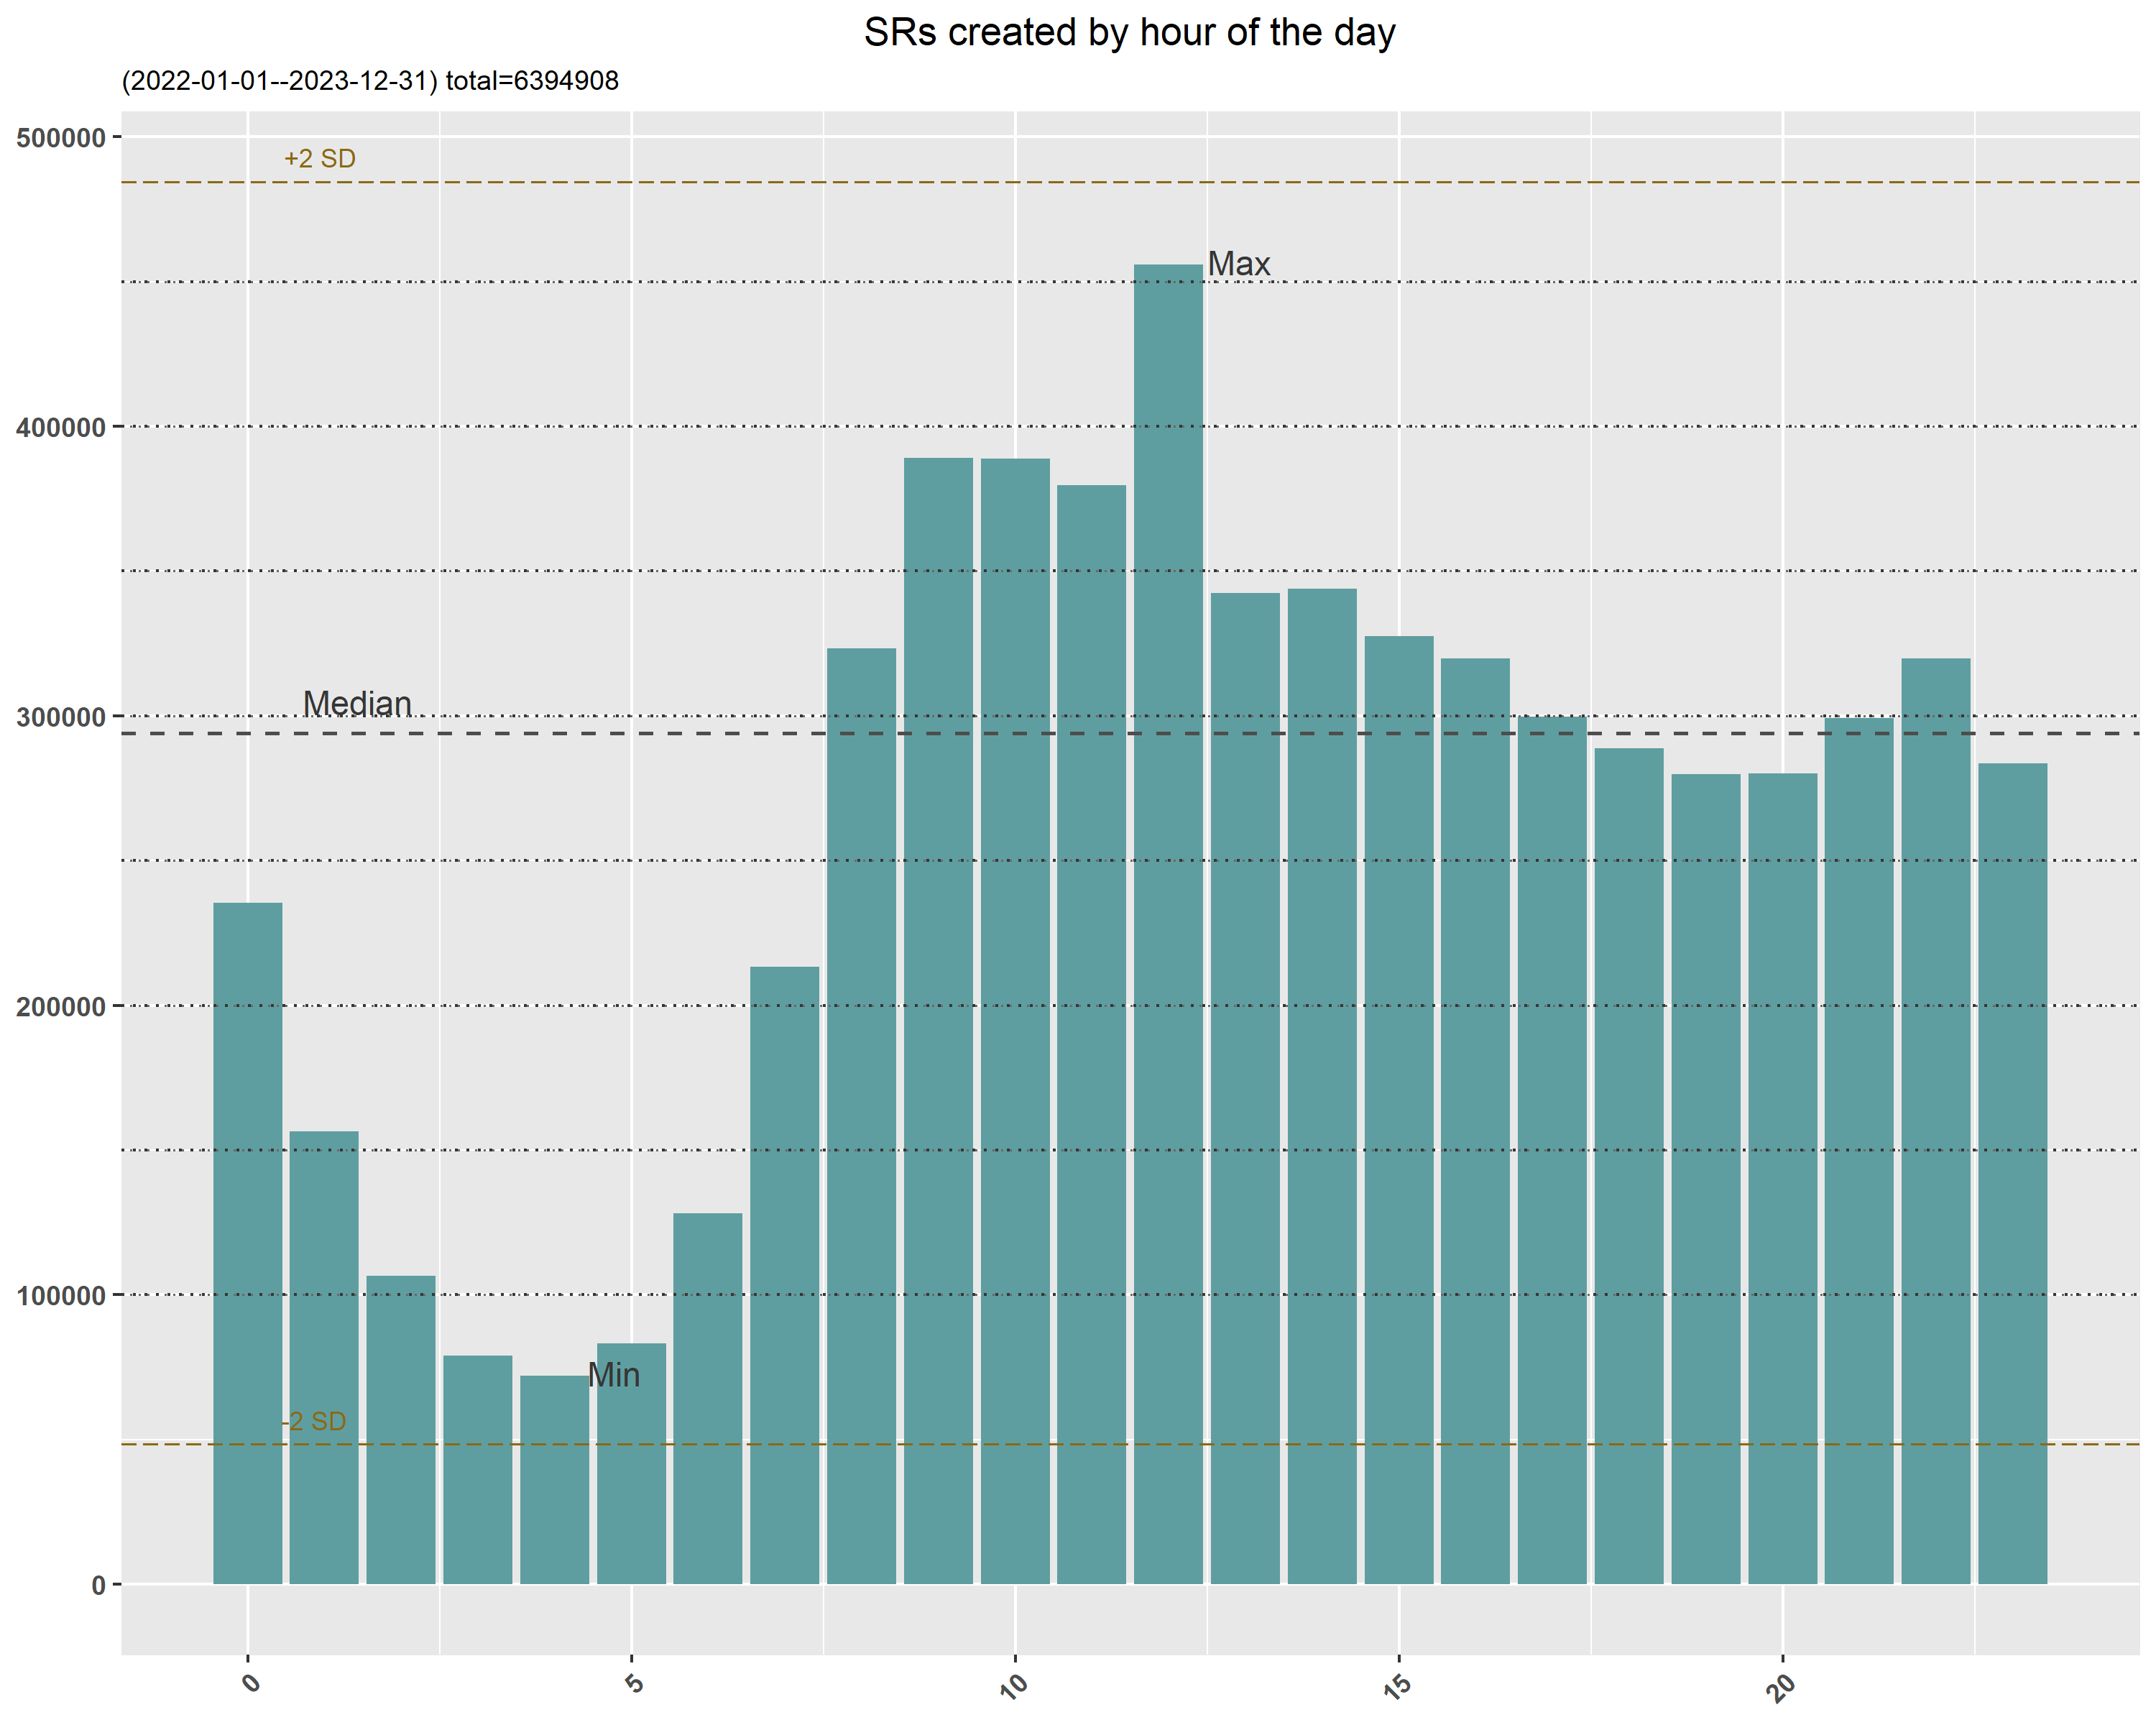
\includegraphics[scale = 0.65]{Created_Hourly_SR_count.png}
		 \caption{SRs by Hourly created\_date(s)}
		 \label{fig:hourly-created}
	\end{figure}	
	
	\begin{figure}[H]
		 \centering
		 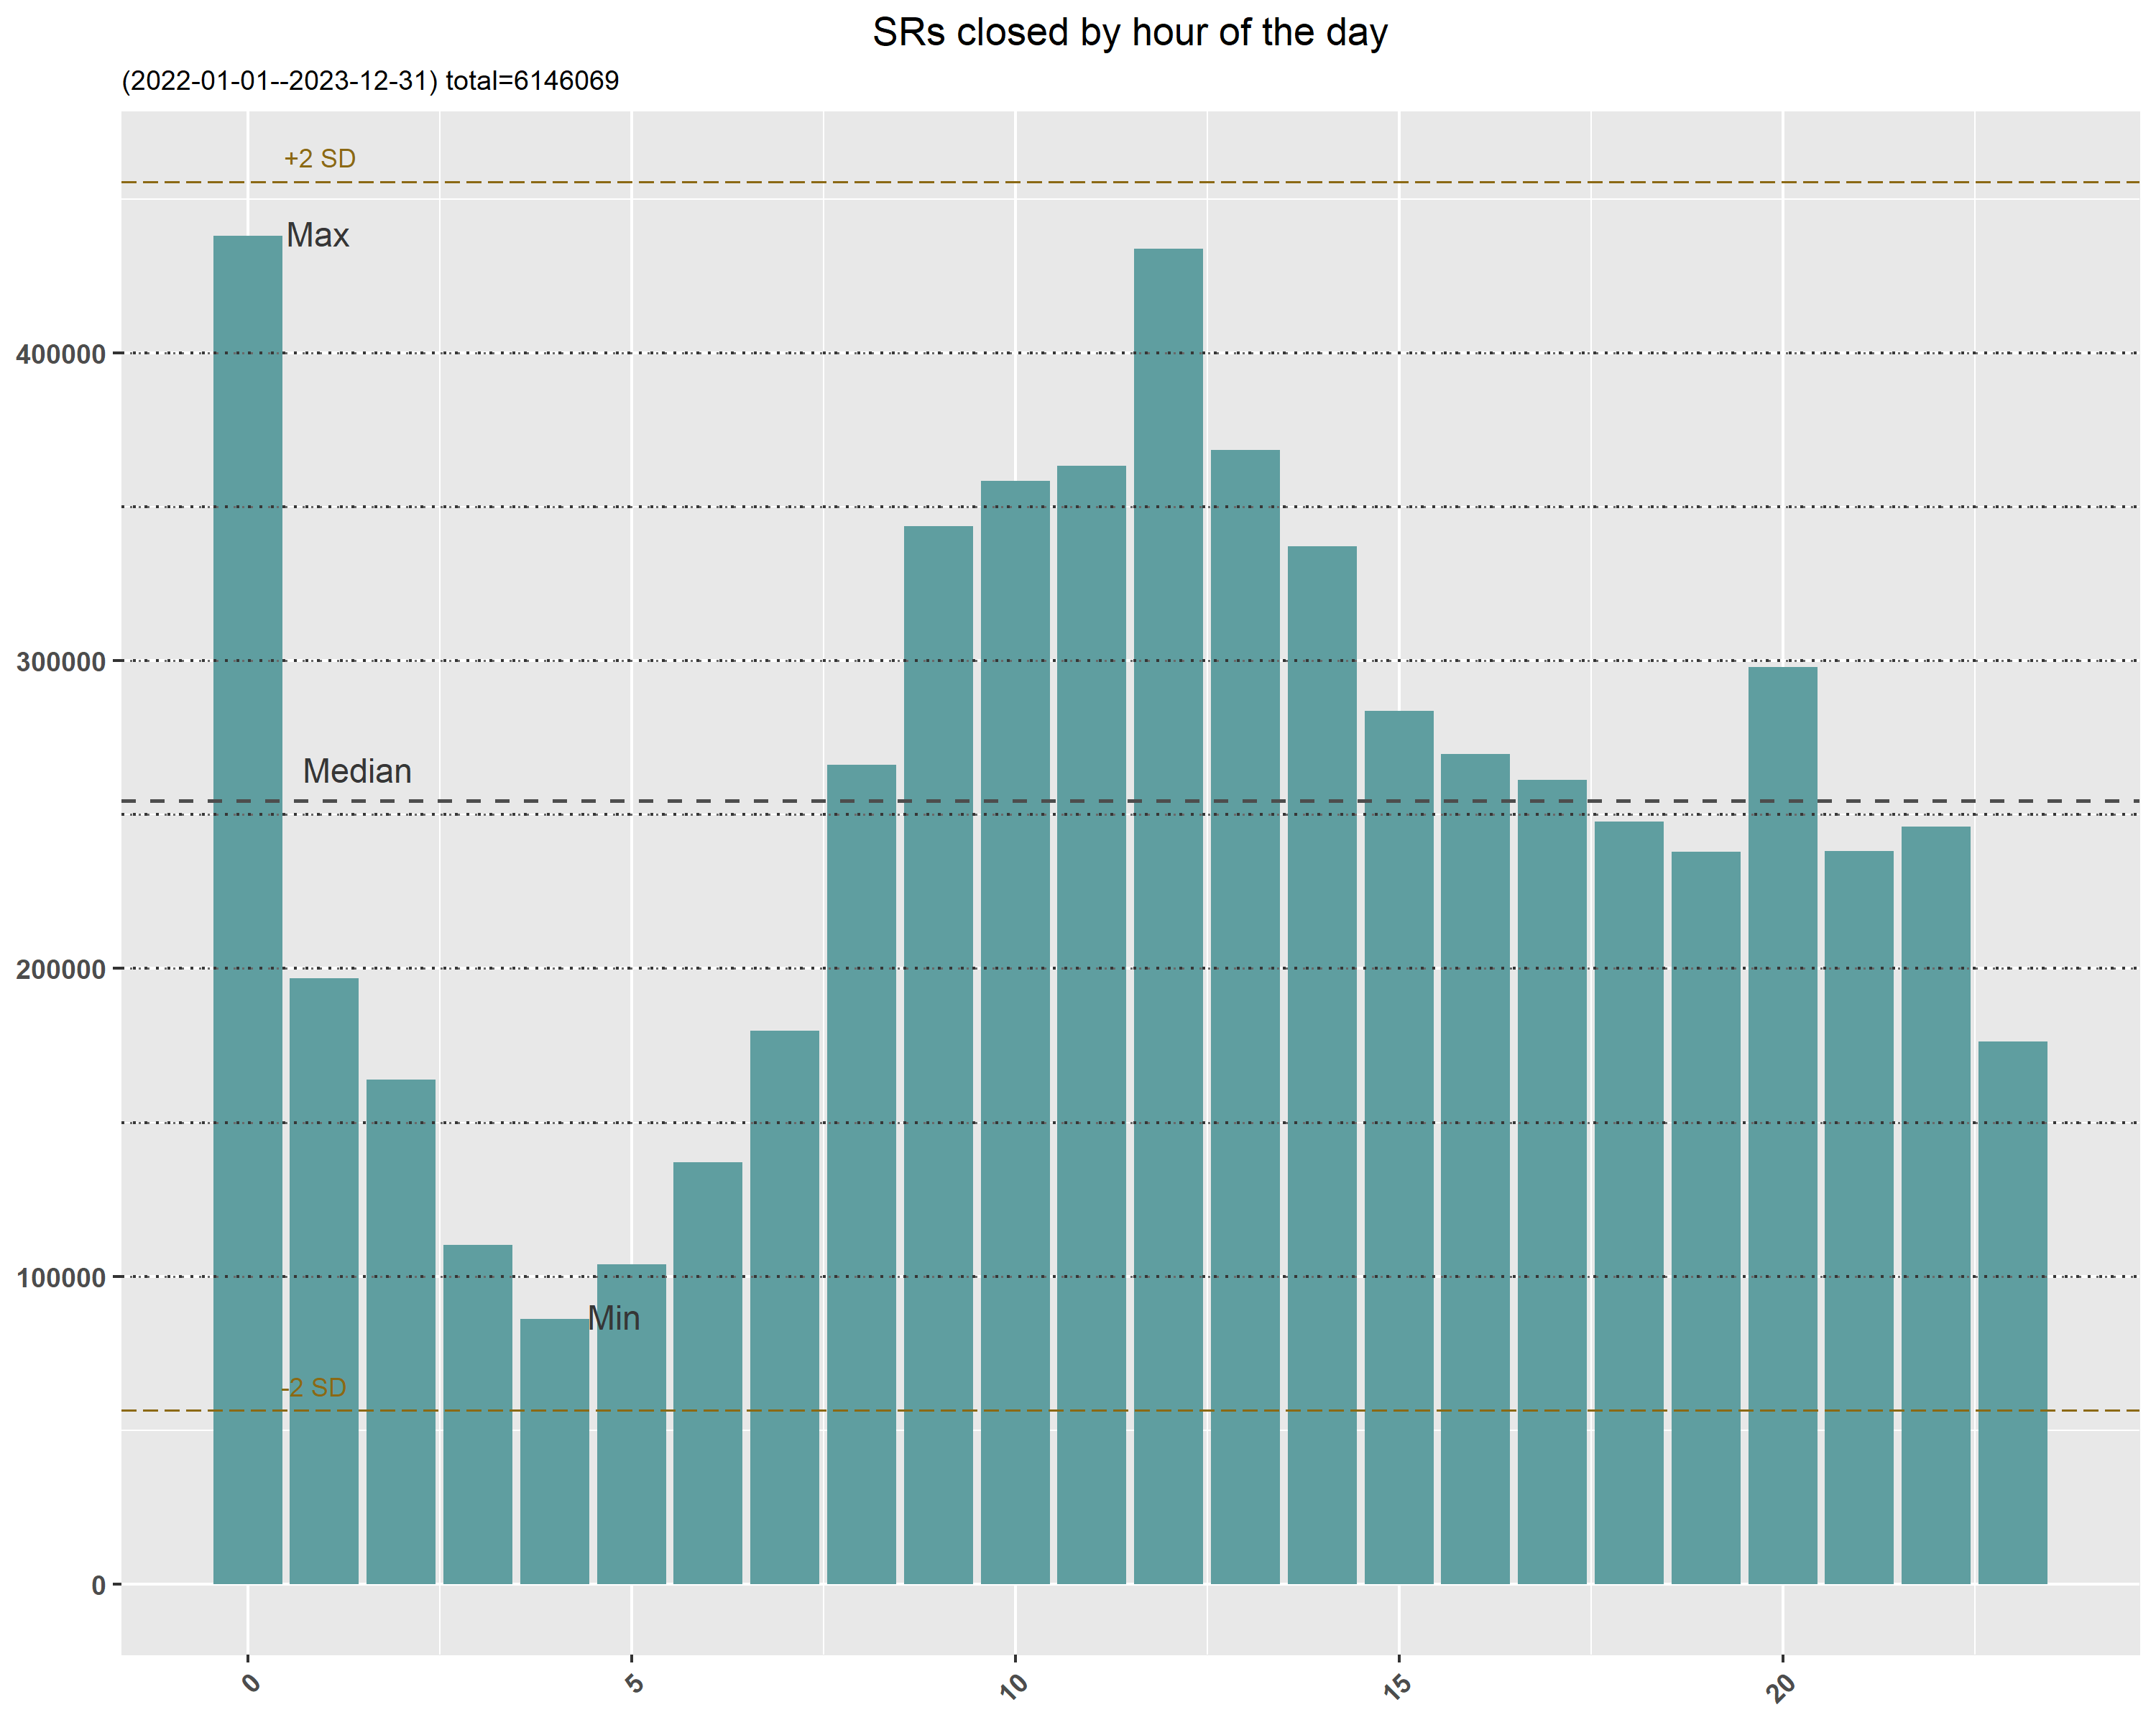
\includegraphics[scale = 0.65]{Closed_Hourly_SR_count.png}
		 \caption{SRs by Hourly closed\_date(s)}
		 \label{fig:hourly-closed}
	\end{figure}	
	
	These ``closed'' charts clearly show significant spikes in the number of SRs at both midnight
	and noon. The midnight spike is clearly out of line with the hours before and after midnight. And
	both the closed-at-noon and closed-at-midnight are approaching 2 standard deviations from the average.

	These unusual patterns of created \& closed SRs on exactly the hours of midnight and noon likely indicate
	some kind of bulk process that perhaps automatically ``closes'' a large number of SRs with a provided
	time-stamp of midnight 00:00:00 or noon 12:00:00. Perhaps there is a similar situation for the ``created'' 
	SRs. So to correct this issue likely requires a close look at what Agencies are providing these suspect SR closed/created times?

	It is not an obvious answer. A visualization of the ``SRs closed at midnight'' shows a distribution that closely mirrors
	the overall assignment of SRs, as the so-called ``Big Six'' Agencies dominate.
	
	\begin{figure}[H]
		 \centering
		 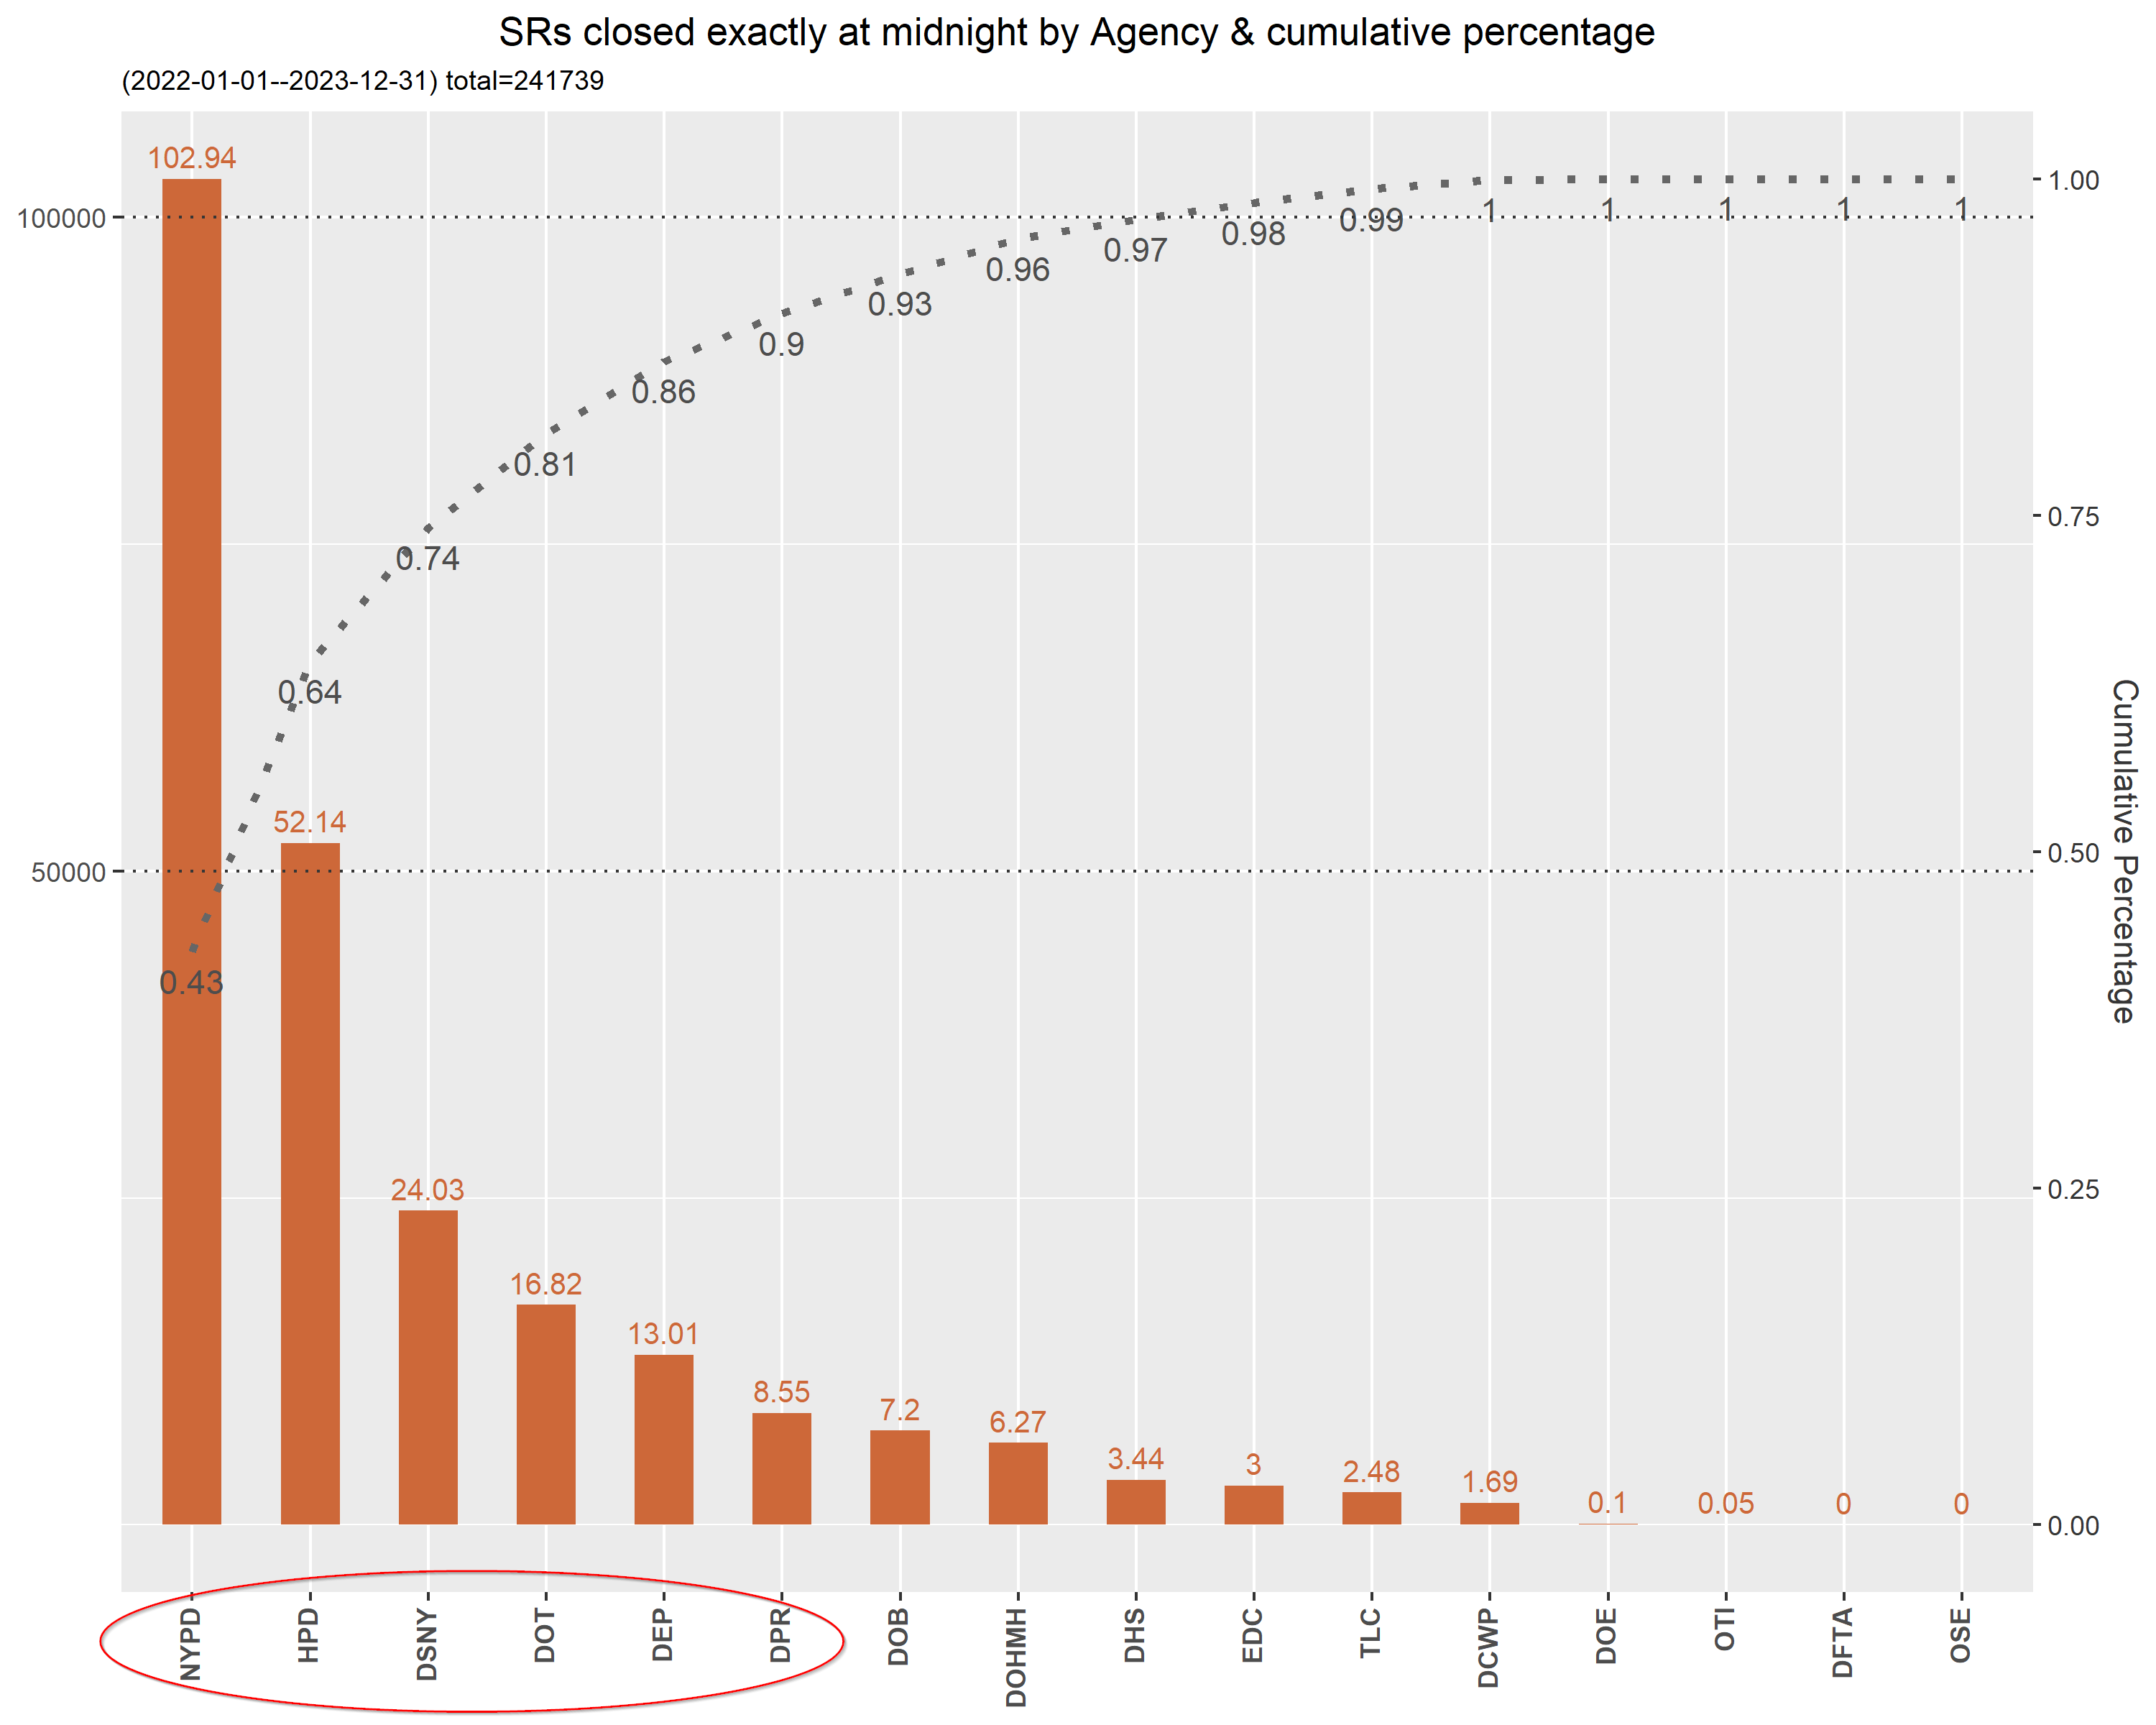
\includegraphics[scale = 0.65]{closed_at_midnight_chart.png}
		 \caption{SRs closed at Midnight by Agency}
		 \label{fig:midnight-closed}
	\end{figure}	
	
	But the ``SR closed at noon'' visualization shows that just a single Agency, Dept of Sanitation (DSNY),
	is responsible for > 99\% of the SRs closed exactly at noon. This indicates that it is necessary
	to work with DSNY to fully understand what is happening. 
	
	\begin{figure}[H]
		 \centering
		 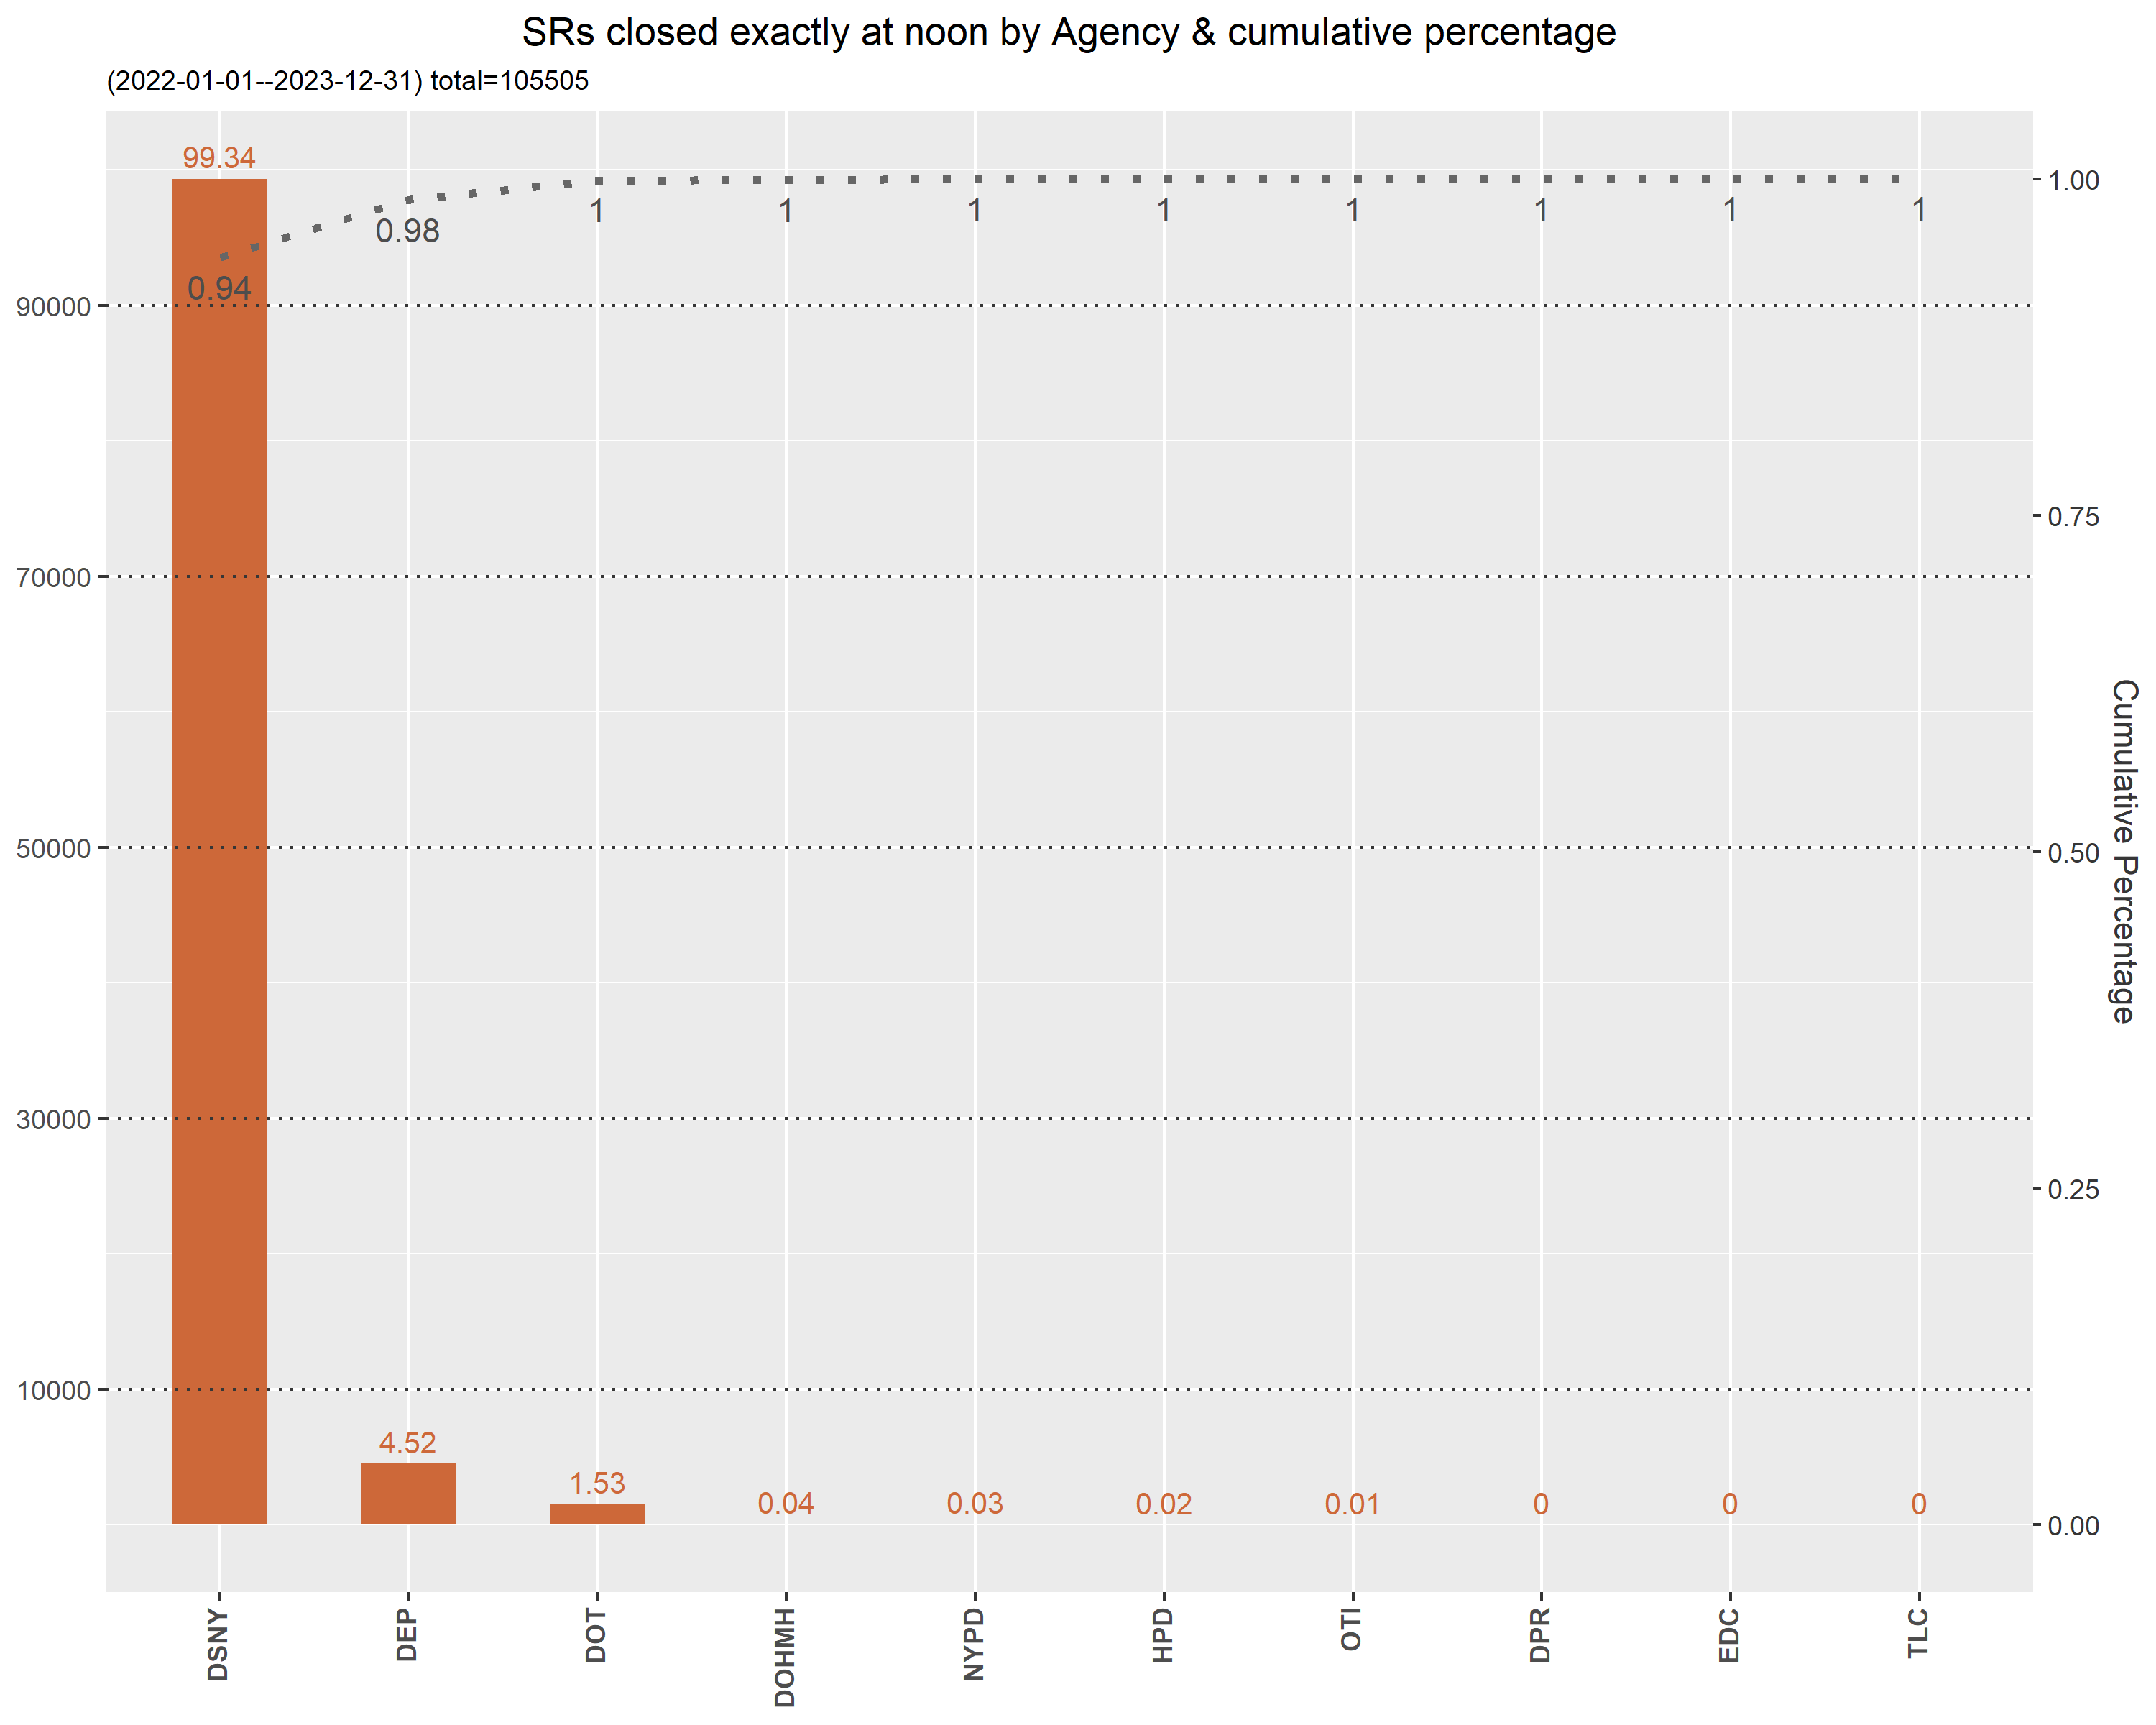
\includegraphics[scale = 0.65]{closed_at_noon_chart.png}
		 \caption{SRs closed at Noon by Agency}
		 \label{fig:noon-closed}
	\end{figure}	
	
		
		
		
		
		
		
		
		
	\subsection{resolution\_action\_update\_date}




\section{Accuracy and precision}\label{sec:precision}
There is one area in particular where the question of precision vs. accuracy immediately arises, and that is with the Latitude and Longitude fields.  Both the 
Longitude and Latitude fields are expresses as a 14-decimal number, e.g. 40.86769186022511 (also the Location field which is a straight concatenation of
latitude and longitude). Given that 1 degree of latitude at the equator is equal to 111.044736 kilometers, the ``1'' at the end of that number represents
approximate 1.1104 nanometer or 1/1,000,000,000 of a meter. A DNA molecule is approximately 2nm in width. 

Clearly the representation of the Latitude and Longitude fields are a classic case of 14-digit precision, 
but limited accuracy. It is more likely that the Lat/Long values are accurate to the 5\textsuperscript{th} decimal place, about 3.64 feet; even that might be
overstating things. 

\subsection{Case Study I - Response to Requests for Homeless Person Assistance}



\section{Redundant \& Duplicate data}\label{sec:duplicates}
Shrinking file size by deleting these 11 redundant fields:
     1 - agency\_name 
     2 - park\_borough 
     3 - borough\_boundaries 
     4 - location 
     5 - intersection\_street\_1 
     6 - intersection\_street\_2 
     7 - police\_precinct 
     8 - duration 
     9 - postClosedUpdateDuration 
     10 - translated\_borough\_boundaries 
     11 - zip\_codes 
Original size: 3.2 Gb 
Size after removing redundant columns: 2.8 Gb 
Potential size reduction: 395.3 Mb or 12.3



\section{Improvements} \label{sec:improvements}

Data validation: identify invalid data

Data cleaning: convert to all lower/upper cases;

Data organization: put zipcode/borough in a separate table; verify intersection
== cross; remove redundant columns (and compare how much space saved)



\section{Protocol Suggestions} \label{sec:protocol}



\section{Discussion} \label{sec:discussion}


\bibliographystyle{asa}
\bibliography{ref}

\end{document}




\end{document}
